\documentclass[twoside]{book}

% Packages required by doxygen
\usepackage{fixltx2e}
\usepackage{calc}
\usepackage{doxygen}
\usepackage[export]{adjustbox} % also loads graphicx
\usepackage{graphicx}
\usepackage[utf8]{inputenc}
\usepackage{makeidx}
\usepackage{multicol}
\usepackage{multirow}
\PassOptionsToPackage{warn}{textcomp}
\usepackage{textcomp}
\usepackage[nointegrals]{wasysym}
\usepackage[table]{xcolor}

% NLS support packages
\usepackage[spanish]{babel}
% Font selection
\usepackage[T1]{fontenc}
\usepackage[scaled=.90]{helvet}
\usepackage{courier}
\usepackage{amssymb}
\usepackage{sectsty}
\renewcommand{\familydefault}{\sfdefault}
\allsectionsfont{%
  \fontseries{bc}\selectfont%
  \color{darkgray}%
}
\renewcommand{\DoxyLabelFont}{%
  \fontseries{bc}\selectfont%
  \color{darkgray}%
}
\newcommand{\+}{\discretionary{\mbox{\scriptsize$\hookleftarrow$}}{}{}}

% Page & text layout
\usepackage{geometry}
\geometry{%
  a4paper,%
  top=2.5cm,%
  bottom=2.5cm,%
  left=2.5cm,%
  right=2.5cm%
}
\tolerance=750
\hfuzz=15pt
\hbadness=750
\setlength{\emergencystretch}{15pt}
\setlength{\parindent}{0cm}
\setlength{\parskip}{3ex plus 2ex minus 2ex}
\makeatletter
\renewcommand{\paragraph}{%
  \@startsection{paragraph}{4}{0ex}{-1.0ex}{1.0ex}{%
    \normalfont\normalsize\bfseries\SS@parafont%
  }%
}
\renewcommand{\subparagraph}{%
  \@startsection{subparagraph}{5}{0ex}{-1.0ex}{1.0ex}{%
    \normalfont\normalsize\bfseries\SS@subparafont%
  }%
}
\makeatother

% Headers & footers
\usepackage{fancyhdr}
\pagestyle{fancyplain}
\fancyhead[LE]{\fancyplain{}{\bfseries\thepage}}
\fancyhead[CE]{\fancyplain{}{}}
\fancyhead[RE]{\fancyplain{}{\bfseries\leftmark}}
\fancyhead[LO]{\fancyplain{}{\bfseries\rightmark}}
\fancyhead[CO]{\fancyplain{}{}}
\fancyhead[RO]{\fancyplain{}{\bfseries\thepage}}
\fancyfoot[LE]{\fancyplain{}{}}
\fancyfoot[CE]{\fancyplain{}{}}
\fancyfoot[RE]{\fancyplain{}{\bfseries\scriptsize Generado por Doxygen }}
\fancyfoot[LO]{\fancyplain{}{\bfseries\scriptsize Generado por Doxygen }}
\fancyfoot[CO]{\fancyplain{}{}}
\fancyfoot[RO]{\fancyplain{}{}}
\renewcommand{\footrulewidth}{0.4pt}
\renewcommand{\chaptermark}[1]{%
  \markboth{#1}{}%
}
\renewcommand{\sectionmark}[1]{%
  \markright{\thesection\ #1}%
}

% Indices & bibliography
\usepackage{natbib}
\usepackage[titles]{tocloft}
\setcounter{tocdepth}{3}
\setcounter{secnumdepth}{5}
\makeindex

% Hyperlinks (required, but should be loaded last)
\usepackage{ifpdf}
\ifpdf
  \usepackage[pdftex,pagebackref=true]{hyperref}
\else
  \usepackage[ps2pdf,pagebackref=true]{hyperref}
\fi
\hypersetup{%
  colorlinks=true,%
  linkcolor=blue,%
  citecolor=blue,%
  unicode%
}

% Custom commands
\newcommand{\clearemptydoublepage}{%
  \newpage{\pagestyle{empty}\cleardoublepage}%
}

\usepackage{caption}
\captionsetup{labelsep=space,justification=centering,font={bf},singlelinecheck=off,skip=4pt,position=top}

%===== C O N T E N T S =====

\begin{document}

% Titlepage & ToC
\hypersetup{pageanchor=false,
             bookmarksnumbered=true,
             pdfencoding=unicode
            }
\pagenumbering{alph}
\begin{titlepage}
\vspace*{7cm}
\begin{center}%
{\Large Arboles A\+VL \\[1ex]\large 1.\+0 }\\
\vspace*{1cm}
{\large Generado por Doxygen 1.8.13}\\
\end{center}
\end{titlepage}
\clearemptydoublepage
\pagenumbering{roman}
\tableofcontents
\clearemptydoublepage
\pagenumbering{arabic}
\hypersetup{pageanchor=true}

%--- Begin generated contents ---
\chapter{Equipo 3 -\/ Integrantes}
\label{index}\hypertarget{index}{}\begin{center}  \tabulinesep=1mm
\begin{longtabu} spread 0pt [c]{*{2}{|X[-1]}|}
\hline
\begin{center}\end{center} &\begin{center}\end{center}  \\\cline{1-2}
\PBS\centering {\itshape {\bfseries Facultad de Ciencias de la Computación}}&\PBS\centering {\itshape {\bfseries Benemérita Universidad Autónoma de Puebla}} \\\cline{1-2}
\multicolumn{2}{|p{(\linewidth-\tabcolsep*2-\arrayrulewidth*1)*2/2}|}{\PBS\centering {\bfseries Profesora} María del Carmen Santiago Díaz }\\\cline{1-2}
\multicolumn{2}{|p{(\linewidth-\tabcolsep*2-\arrayrulewidth*1)*2/2}|}{\PBS\centering Estructuras de Datos }\\\cline{1-2}
\multicolumn{2}{|p{(\linewidth-\tabcolsep*2-\arrayrulewidth*1)*2/2}|}{\PBS\centering {\itshape {\bfseries Manual técnico de T\+D\+As y Árboles A\+VL}} }\\\cline{1-2}
\end{longtabu}
~\newline
 \tabulinesep=1mm
\begin{longtabu} spread 0pt [c]{*{2}{|X[-1]}|}
\hline
\rowcolor{\tableheadbgcolor}\multicolumn{2}{|p{(\linewidth-\tabcolsep*2-\arrayrulewidth*1)*2/2}|}{\cellcolor{\tableheadbgcolor}\textbf{ Integrantes del equipo 3 }}\\\cline{1-2}
\endfirsthead
\hline
\endfoot
\hline
\rowcolor{\tableheadbgcolor}\multicolumn{2}{|p{(\linewidth-\tabcolsep*2-\arrayrulewidth*1)*2/2}|}{\cellcolor{\tableheadbgcolor}\textbf{ Integrantes del equipo 3 }}\\\cline{1-2}
\endhead
Batres Pedroza Alejandro&201836943 \\\cline{1-2}
García González Jorge&201847512 \\\cline{1-2}
Méndez Méndez Sebastián&201836190 \\\cline{1-2}
Segura Cuanalo Ricardo Alejandro&201848777 \\\cline{1-2}
\end{longtabu}
~\newline
 \subsection*{Introducción}\end{center} 

\begin{center} Este manual técnico fue realizado con el propósito de brindar una mejor comprensión para cualquiera que busque utilizar nuestros T\+D\+As, ya que esto podría ayudar al usuario a emplear nuestros algoritmos para diferentes tareas. Esto se pretende lograr, utilizando descripciones concisas para los métodos empleados, los parámetros de estos y las variables que contiene cada clase utilizada en el código.   \end{center} 

\begin{center}Ejecutables\+: \href{https://github.com/fcc-2018/arboles-avl/raw/master/ejecutables/arbolAVL.exe}{\tt Windows} -- \href{https://github.com/fcc-2018/arboles-avl/raw/master/ejecutables/arbolAVL}{\tt Linux}\end{center} 

\begin{center}  \end{center}  
\chapter{Indice de namespaces}
\section{Lista de \textquotesingle{}namespaces\textquotesingle{}}
Lista de toda la documentación de los \textquotesingle{}namespaces\textquotesingle{}, con una breve descripción\+:\begin{DoxyCompactList}
\item\contentsline{section}{\hyperlink{namespacecu}{cu} \\*Espacio de nombres destinado a funciones utilizadas en la depuración de las funciones en estudio }{\pageref{namespacecu}}{}
\end{DoxyCompactList}

\chapter{Indice jerárquico}
\section{Jerarquía de la clase}
Esta lista de herencias esta ordenada aproximadamente por orden alfabético\+:\begin{DoxyCompactList}
\item Grafo\begin{DoxyCompactList}
\item \contentsline{section}{Arbol}{\pageref{classArbol}}{}
\end{DoxyCompactList}
\end{DoxyCompactList}

\chapter{Índice de clases}
\section{Lista de clases}
Lista de las clases, estructuras, uniones e interfaces con una breve descripción\+:\begin{DoxyCompactList}
\item\contentsline{section}{\hyperlink{classArbol}{Arbol} \\*Implementación de un árbol binario con listas de adyacencia. ~\newline
 }{\pageref{classArbol}}{}
\item\contentsline{section}{\hyperlink{classArbolAVL}{Arbol\+A\+VL} \\*Implementación de un arbol binario que por cada inserción se corrobore el balance del mismo y se pueda auto-\/balancear }{\pageref{classArbolAVL}}{}
\item\contentsline{section}{\hyperlink{classArista}{Arista} \\*Clase que lleva el control del vertice de \textquotesingle{}origen\textquotesingle{} y de \textquotesingle{}destino\textquotesingle{} y el peso del camino entre estos }{\pageref{classArista}}{}
\item\contentsline{section}{\hyperlink{classcola}{cola$<$ T\+I\+P\+O $>$} \\*Clase que contiene las operaciones de una cola, haciendo uso de templates }{\pageref{classcola}}{}
\item\contentsline{section}{\hyperlink{classEtiqueta}{Etiqueta} \\*Clase de apoyo para conservar el Vértice Origen y su Peso }{\pageref{classEtiqueta}}{}
\item\contentsline{section}{\hyperlink{classGrafo}{Grafo} \\*Clase que contiene todos los procesos que se pueden realizar en el \hyperlink{classGrafo}{Grafo} }{\pageref{classGrafo}}{}
\item\contentsline{section}{\hyperlink{classLista_1_1iterator}{Lista$<$ tipo $>$\+::iterator} }{\pageref{classLista_1_1iterator}}{}
\item\contentsline{section}{\hyperlink{classLista}{Lista$<$ tipo $>$} }{\pageref{classLista}}{}
\item\contentsline{section}{\hyperlink{classMenu}{Menu} \\*Muestra un menu de opciones automaticamente y ejecuta el codigo que se le indica mediante funciones lambda en cada opcion }{\pageref{classMenu}}{}
\item\contentsline{section}{\hyperlink{classLista_1_1Nodo}{Lista$<$ tipo $>$\+::\+Nodo} }{\pageref{classLista_1_1Nodo}}{}
\item\contentsline{section}{\hyperlink{classnodo}{nodo$<$ T\+I\+P\+O $>$} \\*Clase que maneja los atributos escenciales de un nodo, haciendo uso de templates }{\pageref{classnodo}}{}
\item\contentsline{section}{\hyperlink{classnodos}{nodos$<$ T\+I\+P\+O $>$} }{\pageref{classnodos}}{}
\item\contentsline{section}{\hyperlink{classOpcion}{Opcion} \\*Representa a una opcion en el menu del programa }{\pageref{classOpcion}}{}
\item\contentsline{section}{\hyperlink{classpila}{pila$<$ T\+I\+P\+O $>$} }{\pageref{classpila}}{}
\item\contentsline{section}{\hyperlink{classVertice}{Vertice} \\*Clase encargada de llenar los datos en los Nodos insertados al \hyperlink{classGrafo}{Grafo} }{\pageref{classVertice}}{}
\end{DoxyCompactList}

\chapter{Indice de archivos}
\section{Lista de archivos}
Lista de todos los archivos documentados y con descripciones breves\+:\begin{DoxyCompactList}
\item\contentsline{section}{\hyperlink{arbol_8h}{arbol.\+h} }{\pageref{arbol_8h}}{}
\end{DoxyCompactList}

\chapter{Documentación de namespaces}
\hypertarget{namespacecu}{}\section{Referencia del Namespace cu}
\label{namespacecu}\index{cu@{cu}}


Espacio de nombres destinado a funciones utilizadas en la depuración de las funciones en estudio.  


\subsection*{Funciones}
\begin{DoxyCompactItemize}
\item 
void \hyperlink{namespacecu_a2032e7d323896144cae02cca83ea7776}{test} (std\+::string str)
\begin{DoxyCompactList}\small\item\em Muestra en consola el texto pasado como parámetro. \end{DoxyCompactList}\item 
void \hyperlink{namespacecu_a29c88a60e2e11b522402097bac91dd53}{test} (std\+::string str, std\+::string str2)
\begin{DoxyCompactList}\small\item\em Muestra en consola los textos pasados como parámetro. \end{DoxyCompactList}\item 
void \hyperlink{namespacecu_a204c06884ca90cec812a74a79978ad1b}{test} (std\+::string str, int dato)
\begin{DoxyCompactList}\small\item\em Muestra en consola una descripción y un valor dados. \end{DoxyCompactList}\item 
void \hyperlink{namespacecu_ac74aabcdeff59ad38de0aa36237f8a9b}{test} (std\+::string str, int dato, int res)
\begin{DoxyCompactList}\small\item\em Muestra en consola una descripción junto con un valor inicial y un valor como resultado. \end{DoxyCompactList}\item 
void \hyperlink{namespacecu_a4f3e4a3066ea798b15af01022a14ecf9}{test} (std\+::string str, bool cond, std\+::string msg1, std\+::string msg2)
\begin{DoxyCompactList}\small\item\em Muestra en consola una descripción y, según un valor booleano, decide qué texto mostrar después. \end{DoxyCompactList}\item 
void \hyperlink{namespacecu_af2ea0a4da4f2192d226ca8c3bddbd821}{test} (std\+::string str, bool cond)
\begin{DoxyCompactList}\small\item\em Muestra en consola una descripción y, dependiendo del valor booleano dado, mostrará un mensaje \char`\"{}\+Y\+E\+S\char`\"{} o un mensaje \char`\"{}\+N\+O\char`\"{}. \end{DoxyCompactList}\end{DoxyCompactItemize}
\subsection*{Variables}
\begin{DoxyCompactItemize}
\item 
\mbox{\Hypertarget{namespacecu_a67ef22d5c0f232da615812d7c61846a2}\label{namespacecu_a67ef22d5c0f232da615812d7c61846a2}} 
std\+::string \hyperlink{namespacecu_a67ef22d5c0f232da615812d7c61846a2}{promt} = \char`\"{}\mbox{[}D\+E\+B\+UG\mbox{]}\char`\"{}
\begin{DoxyCompactList}\small\item\em Texto que indica que se hace referencia a un texto del depurador. \end{DoxyCompactList}\item 
\mbox{\Hypertarget{namespacecu_ae84c5e905dd7b8c2b1b1194553f9c9a9}\label{namespacecu_ae84c5e905dd7b8c2b1b1194553f9c9a9}} 
bool \hyperlink{namespacecu_ae84c5e905dd7b8c2b1b1194553f9c9a9}{debug\+\_\+mode} = true
\begin{DoxyCompactList}\small\item\em Booleano que indica si el modo depurador está activado o no, es decir, si está en {\itshape true} o {\itshape false} respectivamente. \end{DoxyCompactList}\end{DoxyCompactItemize}


\subsection{Descripción detallada}
Espacio de nombres destinado a funciones utilizadas en la depuración de las funciones en estudio. 

Contiene funciones {\itshape test} que permiten imprimir de manera más práctica directo a consola mensajes de depuración para monitorear de forma más limpia la ejecución de las funciones de interés 

\subsection{Documentación de las funciones}
\mbox{\Hypertarget{namespacecu_a2032e7d323896144cae02cca83ea7776}\label{namespacecu_a2032e7d323896144cae02cca83ea7776}} 
\index{cu@{cu}!test@{test}}
\index{test@{test}!cu@{cu}}
\subsubsection{\texorpdfstring{test()}{test()}\hspace{0.1cm}{\footnotesize\ttfamily [1/6]}}
{\footnotesize\ttfamily void cu\+::test (\begin{DoxyParamCaption}\item[{std\+::string}]{str }\end{DoxyParamCaption})}



Muestra en consola el texto pasado como parámetro. 


\begin{DoxyParams}{Parámetros}
{\em str} & texto a imprimir en consola \\
\hline
\end{DoxyParams}


Definición en la línea 45 del archivo testing.\+hpp.

\mbox{\Hypertarget{namespacecu_a29c88a60e2e11b522402097bac91dd53}\label{namespacecu_a29c88a60e2e11b522402097bac91dd53}} 
\index{cu@{cu}!test@{test}}
\index{test@{test}!cu@{cu}}
\subsubsection{\texorpdfstring{test()}{test()}\hspace{0.1cm}{\footnotesize\ttfamily [2/6]}}
{\footnotesize\ttfamily void cu\+::test (\begin{DoxyParamCaption}\item[{std\+::string}]{str,  }\item[{std\+::string}]{str2 }\end{DoxyParamCaption})}



Muestra en consola los textos pasados como parámetro. 


\begin{DoxyParams}{Parámetros}
{\em str} & primer texto a imprimir en consola \\
\hline
{\em str2} & segundo texto a imprimir en consola \\
\hline
\end{DoxyParams}


Definición en la línea 54 del archivo testing.\+hpp.

\mbox{\Hypertarget{namespacecu_a204c06884ca90cec812a74a79978ad1b}\label{namespacecu_a204c06884ca90cec812a74a79978ad1b}} 
\index{cu@{cu}!test@{test}}
\index{test@{test}!cu@{cu}}
\subsubsection{\texorpdfstring{test()}{test()}\hspace{0.1cm}{\footnotesize\ttfamily [3/6]}}
{\footnotesize\ttfamily void cu\+::test (\begin{DoxyParamCaption}\item[{std\+::string}]{str,  }\item[{int}]{dato }\end{DoxyParamCaption})}



Muestra en consola una descripción y un valor dados. 


\begin{DoxyParams}{Parámetros}
{\em str} & descripción del valor \\
\hline
{\em dato} & valor numérico \\
\hline
\end{DoxyParams}


Definición en la línea 63 del archivo testing.\+hpp.

\mbox{\Hypertarget{namespacecu_ac74aabcdeff59ad38de0aa36237f8a9b}\label{namespacecu_ac74aabcdeff59ad38de0aa36237f8a9b}} 
\index{cu@{cu}!test@{test}}
\index{test@{test}!cu@{cu}}
\subsubsection{\texorpdfstring{test()}{test()}\hspace{0.1cm}{\footnotesize\ttfamily [4/6]}}
{\footnotesize\ttfamily void cu\+::test (\begin{DoxyParamCaption}\item[{std\+::string}]{str,  }\item[{int}]{dato,  }\item[{int}]{res }\end{DoxyParamCaption})}



Muestra en consola una descripción junto con un valor inicial y un valor como resultado. 


\begin{DoxyParams}{Parámetros}
{\em str} & descripción de la operación \\
\hline
{\em dato} & valor numérico inicial \\
\hline
{\em res} & valor numérico resultante \\
\hline
\end{DoxyParams}


Definición en la línea 74 del archivo testing.\+hpp.

\mbox{\Hypertarget{namespacecu_a4f3e4a3066ea798b15af01022a14ecf9}\label{namespacecu_a4f3e4a3066ea798b15af01022a14ecf9}} 
\index{cu@{cu}!test@{test}}
\index{test@{test}!cu@{cu}}
\subsubsection{\texorpdfstring{test()}{test()}\hspace{0.1cm}{\footnotesize\ttfamily [5/6]}}
{\footnotesize\ttfamily void cu\+::test (\begin{DoxyParamCaption}\item[{std\+::string}]{str,  }\item[{bool}]{cond,  }\item[{std\+::string}]{msg1,  }\item[{std\+::string}]{msg2 }\end{DoxyParamCaption})}



Muestra en consola una descripción y, según un valor booleano, decide qué texto mostrar después. 


\begin{DoxyParams}{Parámetros}
{\em str} & descripción de las condiciones \\
\hline
{\em cond} & booleano determinante \\
\hline
{\em msg1} & texto que se mostrará si el valor booleano es {\itshape true} \\
\hline
{\em msg2} & texto que se mostrará si el valor booleano es {\itshape false} \\
\hline
\end{DoxyParams}


Definición en la línea 86 del archivo testing.\+hpp.

\mbox{\Hypertarget{namespacecu_af2ea0a4da4f2192d226ca8c3bddbd821}\label{namespacecu_af2ea0a4da4f2192d226ca8c3bddbd821}} 
\index{cu@{cu}!test@{test}}
\index{test@{test}!cu@{cu}}
\subsubsection{\texorpdfstring{test()}{test()}\hspace{0.1cm}{\footnotesize\ttfamily [6/6]}}
{\footnotesize\ttfamily void cu\+::test (\begin{DoxyParamCaption}\item[{std\+::string}]{str,  }\item[{bool}]{cond }\end{DoxyParamCaption})}



Muestra en consola una descripción y, dependiendo del valor booleano dado, mostrará un mensaje \char`\"{}\+Y\+E\+S\char`\"{} o un mensaje \char`\"{}\+N\+O\char`\"{}. 


\begin{DoxyParams}{Parámetros}
{\em str} & descripción de la condición \\
\hline
{\em cond} & booleano determiante. En caso de ser {\itshape true}, se mostrará \char`\"{}\+Y\+E\+S\char`\"{}. En caso contrario (es decir, {\itshape false}) se mostrará \char`\"{}\+N\+O\char`\"{} \\
\hline
\end{DoxyParams}


Definición en la línea 97 del archivo testing.\+hpp.


\chapter{Documentación de las clases}
\hypertarget{classArbol}{}\section{Referencia de la Clase Arbol}
\label{classArbol}\index{Arbol@{Arbol}}


Implementación de un arbol binario basada en un grafo con listas de adyacencia.  




{\ttfamily \#include $<$arbol.\+h$>$}



Diagrama de herencias de Arbol
% FIG 0


Diagrama de colaboración para Arbol\+:
% FIG 1
\subsection*{Métodos públicos}
\begin{DoxyCompactItemize}
\item 
\mbox{\Hypertarget{classArbol_a4f5d3e25a0e1a40cb09cefa39378b7be}\label{classArbol_a4f5d3e25a0e1a40cb09cefa39378b7be}} 
\hyperlink{classArbol_a4f5d3e25a0e1a40cb09cefa39378b7be}{Arbol} ()
\begin{DoxyCompactList}\small\item\em Constructor de la clase, se asume que la raíz del árbol es el primer vértice en la lista de adyacencia. \end{DoxyCompactList}\item 
int \hyperlink{classArbol_af332559b5f9d894ecc6a707bb1550ae2}{insertar} (int dato)
\begin{DoxyCompactList}\small\item\em Inserta un dato en el árbol. \end{DoxyCompactList}\item 
void \hyperlink{classArbol_a61749974f55056420f4e5a76eb664809}{mostrar} (ostream \&out)
\begin{DoxyCompactList}\small\item\em Muestra el árbol de manera horizontal. \end{DoxyCompactList}\item 
\mbox{\Hypertarget{classArbol_a5bd356760f63521e8578a83613aa4792}\label{classArbol_a5bd356760f63521e8578a83613aa4792}} 
void \hyperlink{classArbol_a5bd356760f63521e8578a83613aa4792}{recorrer} ()
\begin{DoxyCompactList}\small\item\em Muestra el árbol verticalmente. \end{DoxyCompactList}\item 
void \hyperlink{classArbol_a0ae46c572d300cd4a5f27b7d00a1a14e}{recorrer} (Vertice $\ast$raiz, int cont)
\begin{DoxyCompactList}\small\item\em Metodo recursivo auxiliar para \hyperlink{classArbol_a5bd356760f63521e8578a83613aa4792}{recorrer()} \end{DoxyCompactList}\item 
Lista$<$ Vertice $\ast$ $>$ $\ast$ \hyperlink{classArbol_a0ffdc60ce8f2267366681cc94cf6beea}{preorden} ()
\begin{DoxyCompactList}\small\item\em Recorre el árbol en preorden y los inserta en una lista. \end{DoxyCompactList}\item 
Lista$<$ Vertice $\ast$ $>$ $\ast$ \hyperlink{classArbol_a80a0c3cf2d7f3e92a5c8e5504947dab5}{inorden} ()
\begin{DoxyCompactList}\small\item\em Recorre el árbol en inorden y los inserta en una lista. \end{DoxyCompactList}\item 
\mbox{\Hypertarget{classArbol_a126e7d801dbe214ac39f183c26e9135d}\label{classArbol_a126e7d801dbe214ac39f183c26e9135d}} 
Lista$<$ Vertice $\ast$ $>$ $\ast$ \hyperlink{classArbol_a126e7d801dbe214ac39f183c26e9135d}{postorden} ()
\begin{DoxyCompactList}\small\item\em Recorre el árbol en inorden. \end{DoxyCompactList}\item 
int \hyperlink{classArbol_a9051a6b4120b42ff8d046f41ab73dbaa}{peso} ()
\begin{DoxyCompactList}\small\item\em Calcula el número de nodos en el árbol. \end{DoxyCompactList}\item 
int \hyperlink{classArbol_a99e608849650b891c34852a81f93d4ab}{grado} ()
\begin{DoxyCompactList}\small\item\em Calcula el grado del árbol, máximo número de hijos en cada nodo. \end{DoxyCompactList}\item 
Vertice $\ast$ \hyperlink{classArbol_abcb8c26e9021a1418de71ad6014351cf}{padre} (int hijo)
\begin{DoxyCompactList}\small\item\em Obtiene el padre de un nodo. \end{DoxyCompactList}\item 
Vertice $\ast$ \hyperlink{classArbol_a53527e7a8999ceda0b8a0fa25a3f357c}{padre} (string hijo)
\begin{DoxyCompactList}\small\item\em Obtiene el padre de un nodo. \end{DoxyCompactList}\item 
Vertice $\ast$ \hyperlink{classArbol_a3395234bc7b7a91d2880e10367039284}{padre} (Vertice $\ast$hijo)
\begin{DoxyCompactList}\small\item\em Obtiene el padre de un nodo. \end{DoxyCompactList}\item 
Lista$<$ Vertice $\ast$ $>$ $\ast$ \hyperlink{classArbol_ac2bfb4e9bab05342fb7d627fe3916183}{hijos} (int \hyperlink{classArbol_abcb8c26e9021a1418de71ad6014351cf}{padre})
\begin{DoxyCompactList}\small\item\em Obtiene los hijos de un vértice. \end{DoxyCompactList}\item 
Lista$<$ Vertice $\ast$ $>$ $\ast$ \hyperlink{classArbol_ac799e737e25e07d285d2bb29ba950b5c}{hijos} (string \hyperlink{classArbol_abcb8c26e9021a1418de71ad6014351cf}{padre})
\begin{DoxyCompactList}\small\item\em Obtiene los hijos de un vértice. \end{DoxyCompactList}\item 
Lista$<$ Vertice $\ast$ $>$ $\ast$ \hyperlink{classArbol_a54203315682d5c39015ae7d871223b66}{hojas} ()
\begin{DoxyCompactList}\small\item\em Obtiene las hojas del árbol. \end{DoxyCompactList}\item 
int \hyperlink{classArbol_aba59969b2a10294fb79e583a8e9471c5}{cont\+\_\+hojas} (Vertice $\ast$raiz)
\begin{DoxyCompactList}\small\item\em Calcula el número de hojas en el árbol. \end{DoxyCompactList}\item 
Vertice $\ast$ \hyperlink{classArbol_a59ae16f1a68c5e5afd08be20dcbf5717}{hermano} (int buscar)
\begin{DoxyCompactList}\small\item\em Obtiene el hermano de un vértice. \end{DoxyCompactList}\item 
bool \hyperlink{classArbol_a14ccdbb79a82bf19a24449acaea6c413}{es\+\_\+lleno} ()
\begin{DoxyCompactList}\small\item\em Verifica si el árbol cumple las condiciones de un árbol lleno, es decir cada nodo debe tener 0 o 2 hijos. \end{DoxyCompactList}\item 
bool \hyperlink{classArbol_a9e472df85f3bb1aa5c90f8157ad6ff22}{es\+\_\+completo\+\_\+o\+\_\+perfecto} ()
\begin{DoxyCompactList}\small\item\em Verifica si el árbol cumple las condiciones de un árbol perfecto/lleno ( árbol lleno con todas sus hojas en el mismo nivel ) \end{DoxyCompactList}\item 
int \hyperlink{classArbol_a98151655f0dab81b40d34f87fbbd90cd}{altura} (int dato)
\begin{DoxyCompactList}\small\item\em Calcula la altura de un nodo. \end{DoxyCompactList}\item 
int \hyperlink{classArbol_a7a79cb43ca30b5120f1a8ebe3afbe22c}{altura} (string nombre)
\begin{DoxyCompactList}\small\item\em Calcula la altura de un nodo. \end{DoxyCompactList}\item 
int \hyperlink{classArbol_a9f8928b4c72e2d484ef75cf3633c22ce}{altura} (Vertice $\ast$nodo)
\begin{DoxyCompactList}\small\item\em Calcula la altura de un nodo. \end{DoxyCompactList}\item 
int \hyperlink{classArbol_accd2dd2f8012067c1a2d77fd14c64546}{nivel} (int dato)
\begin{DoxyCompactList}\small\item\em Calcula el nivel donde se encuentra un nodo. \end{DoxyCompactList}\item 
int \hyperlink{classArbol_a3a8a414e8e3f45bf90c481649928a86d}{nivel} (string nombre)
\begin{DoxyCompactList}\small\item\em Calcula el nivel donde se encuentra un nodo. \end{DoxyCompactList}\item 
Lista$<$ Vertice $\ast$ $>$ $\ast$ \hyperlink{classArbol_ac7ff5e2f436a1e83e24cbdd0b2cc827b}{antecesores} (int dato)
\begin{DoxyCompactList}\small\item\em Obtiene los antecesores de un nodo. \end{DoxyCompactList}\item 
Lista$<$ Vertice $\ast$ $>$ $\ast$ \hyperlink{classArbol_aa975d5d9cf5fcfc392a8200bd0078d1c}{antecesores} (string nombre)
\begin{DoxyCompactList}\small\item\em Obtiene los antecesores de un nodo. \end{DoxyCompactList}\item 
Lista$<$ Vertice $\ast$ $>$ $\ast$ \hyperlink{classArbol_acae8e9dfd17ae18e250d9029172e1c9e}{descendientes} (int dato)
\begin{DoxyCompactList}\small\item\em Obtiene los descendientes de un nodo. \end{DoxyCompactList}\item 
Lista$<$ Vertice $\ast$ $>$ $\ast$ \hyperlink{classArbol_a790b07f284b14bd179499eb4a991ad86}{descendientes} (string nombre)
\begin{DoxyCompactList}\small\item\em Obtiene los descendientes de un nodo. \end{DoxyCompactList}\item 
Lista$<$ Vertice $\ast$ $>$ $\ast$ \hyperlink{classArbol_accfa606c5f5e67b6ab18c4490075cf39}{camino\+\_\+entre} (int o, int d)
\begin{DoxyCompactList}\small\item\em Obtiene el un camino entre dos vértices en el árbol. \end{DoxyCompactList}\item 
Lista$<$ Vertice $\ast$ $>$ $\ast$ \hyperlink{classArbol_aef0f680828ac573af495b98d2eb09c12}{camino\+\_\+entre} (string origen, string destino)
\begin{DoxyCompactList}\small\item\em Obtiene el un camino entre dos vértices en el árbol. \end{DoxyCompactList}\end{DoxyCompactItemize}
\subsection*{Métodos protegidos}
\begin{DoxyCompactItemize}
\item 
void \hyperlink{classArbol_a707f748c57d51f6b63fe1a605476e49d}{\+\_\+\+\_\+preorden\+\_\+\+\_\+} (Vertice $\ast$raiz, Lista$<$ Vertice $\ast$$>$ $\ast$lista)
\begin{DoxyCompactList}\small\item\em Recorre un árbol en preorden (Visitar, Izquierda, Derecha) recursivamente, método auxiliar de \hyperlink{classArbol_a0ffdc60ce8f2267366681cc94cf6beea}{preorden()} \end{DoxyCompactList}\item 
void \hyperlink{classArbol_ae3dc89f7db1fb9b54bcc2489eb1d9542}{\+\_\+\+\_\+inorden\+\_\+\+\_\+} (Vertice $\ast$raiz, Lista$<$ Vertice $\ast$$>$ $\ast$lista)
\begin{DoxyCompactList}\small\item\em Recorre un árbol en inorden (Izquierda, Visitar, Derecha) recursivamente, método auxiliar de \hyperlink{classArbol_a80a0c3cf2d7f3e92a5c8e5504947dab5}{inorden()} \end{DoxyCompactList}\item 
void \hyperlink{classArbol_aea4cc9147a79d74956413a233df1dbe0}{\+\_\+\+\_\+postorden\+\_\+\+\_\+} (Vertice $\ast$raiz, Lista$<$ Vertice $\ast$$>$ $\ast$lista)
\begin{DoxyCompactList}\small\item\em Recorre un árbol en postorden (Izquierda, Derecha, Visitar) recursivamente, método auxiliar de \hyperlink{classArbol_a126e7d801dbe214ac39f183c26e9135d}{postorden()} \end{DoxyCompactList}\item 
void \hyperlink{classArbol_a1e00baa76d846e9e586e7d179ec51907}{\+\_\+\+\_\+camino\+\_\+\+\_\+} (Vertice $\ast$origen, Vertice $\ast$destino, Lista$<$ Vertice $\ast$$>$ $\ast$$\ast$camino)
\begin{DoxyCompactList}\small\item\em Obtiene el camino entre 2 vértices en el árbol, método auxiliar de \hyperlink{classArbol_accfa606c5f5e67b6ab18c4490075cf39}{camino\+\_\+entre()} \end{DoxyCompactList}\item 
int \hyperlink{classArbol_ad3077ad7b0c57ed7c98baa7fcd8aab47}{\+\_\+\+\_\+grado\+\_\+\+\_\+} (Vertice $\ast$raiz)
\begin{DoxyCompactList}\small\item\em Obtiene el grado de un árbol de manera recursiva. \end{DoxyCompactList}\item 
int \hyperlink{classArbol_ab34b0a58f349a2f8153911ad4821a9b9}{\+\_\+\+\_\+altura\+\_\+\+\_\+} (Vertice $\ast$v)
\begin{DoxyCompactList}\small\item\em Obtiene la altura de un árbol recursivamente. \end{DoxyCompactList}\item 
int \hyperlink{classArbol_a479d9841f100bf75b87fb2155b66d591}{\+\_\+\+\_\+nivel\+\_\+\+\_\+} (Vertice $\ast$raiz, Vertice $\ast$vert, int lvl)
\begin{DoxyCompactList}\small\item\em Obtiene el nivel de un nodo en el árbol. \end{DoxyCompactList}\item 
void \hyperlink{classArbol_aad97c679cb368931b2c6894b3dbcb60f}{\+\_\+\+\_\+hojas\+\_\+\+\_\+} (Vertice $\ast$raiz, Lista$<$ Vertice $\ast$$>$ $\ast$lista)
\begin{DoxyCompactList}\small\item\em Obtiene las hojas de un árbol. \end{DoxyCompactList}\item 
void \hyperlink{classArbol_a1e3da012e6667062976bca9f78efef7e}{\+\_\+\+\_\+hijos\+\_\+\+\_\+} (Vertice $\ast$raiz, Vertice $\ast$\hyperlink{classArbol_abcb8c26e9021a1418de71ad6014351cf}{padre}, Lista$<$ Vertice $\ast$$>$ $\ast$lista)
\begin{DoxyCompactList}\small\item\em Obtiene los hijos de un nodo dado. \end{DoxyCompactList}\item 
void \hyperlink{classArbol_a495a7502a29e01ce7fa168daca651b1f}{\+\_\+\+\_\+padre\+\_\+\+\_\+} (Vertice $\ast$raiz, Vertice $\ast$hijo, Vertice $\ast$$\ast$\hyperlink{classArbol_abcb8c26e9021a1418de71ad6014351cf}{padre})
\begin{DoxyCompactList}\small\item\em Obtiene el padre de un nodo dado. \end{DoxyCompactList}\item 
void \hyperlink{classArbol_aeb7dff584795382d8e8a1a4694d0ac4e}{ordenar\+\_\+lista\+\_\+de\+\_\+adyacentes} (Lista$<$ Vertice $\ast$$>$ $\ast$lista)
\begin{DoxyCompactList}\small\item\em Ordena una lista de vértices en orden ascendente. \end{DoxyCompactList}\item 
Vertice $\ast$$\ast$ \hyperlink{classArbol_a18066699977ab8095398d026ef2a13ac}{obtener\+\_\+hijos} (Vertice $\ast$\hyperlink{classArbol_abcb8c26e9021a1418de71ad6014351cf}{padre})
\begin{DoxyCompactList}\small\item\em Obtiene los hijos de un vértice en orden ascendente. \end{DoxyCompactList}\item 
bool \hyperlink{classArbol_aba4b09fef18152beb43e04fee7394f34}{todos\+\_\+cumplen\+\_\+con} (bool($\ast$funcion\+\_\+callback)(Vertice $\ast$))
\begin{DoxyCompactList}\small\item\em Verifica que todos los vértices en el árbol cumplen una condición dada por una función de callback. \end{DoxyCompactList}\item 
bool \hyperlink{classArbol_a60b71d79b81a3a1083709ec264332975}{\+\_\+\+\_\+todos\+\_\+cumplen\+\_\+con\+\_\+\+\_\+} (bool($\ast$funcion\+\_\+callback)(Vertice $\ast$), Vertice $\ast$vert)
\begin{DoxyCompactList}\small\item\em Método auxiliar para \hyperlink{classArbol_aba4b09fef18152beb43e04fee7394f34}{todos\+\_\+cumplen\+\_\+con()} verifica la condición en cada nodo del árbol recursivamente. \end{DoxyCompactList}\end{DoxyCompactItemize}


\subsection{Descripción detallada}
Implementación de un arbol binario basada en un grafo con listas de adyacencia. 

Definición en la línea 30 del archivo arbol.\+h.



\subsection{Documentación de las funciones miembro}
\mbox{\Hypertarget{classArbol_ab34b0a58f349a2f8153911ad4821a9b9}\label{classArbol_ab34b0a58f349a2f8153911ad4821a9b9}} 
\index{Arbol@{Arbol}!\+\_\+\+\_\+altura\+\_\+\+\_\+@{\+\_\+\+\_\+altura\+\_\+\+\_\+}}
\index{\+\_\+\+\_\+altura\+\_\+\+\_\+@{\+\_\+\+\_\+altura\+\_\+\+\_\+}!Arbol@{Arbol}}
\subsubsection{\texorpdfstring{\+\_\+\+\_\+altura\+\_\+\+\_\+()}{\_\_altura\_\_()}}
{\footnotesize\ttfamily int Arbol\+::\+\_\+\+\_\+altura\+\_\+\+\_\+ (\begin{DoxyParamCaption}\item[{Vertice $\ast$}]{v }\end{DoxyParamCaption})\hspace{0.3cm}{\ttfamily [protected]}}



Obtiene la altura de un árbol recursivamente. 


\begin{DoxyParams}{Parámetros}
{\em v} & puntero a vértice raíz del árbol \\
\hline
\end{DoxyParams}
\begin{DoxyReturn}{Devuelve}
altura del árbol 0 si es hoja 
\end{DoxyReturn}


Definición en la línea 937 del archivo arbol.\+h.

\mbox{\Hypertarget{classArbol_a1e00baa76d846e9e586e7d179ec51907}\label{classArbol_a1e00baa76d846e9e586e7d179ec51907}} 
\index{Arbol@{Arbol}!\+\_\+\+\_\+camino\+\_\+\+\_\+@{\+\_\+\+\_\+camino\+\_\+\+\_\+}}
\index{\+\_\+\+\_\+camino\+\_\+\+\_\+@{\+\_\+\+\_\+camino\+\_\+\+\_\+}!Arbol@{Arbol}}
\subsubsection{\texorpdfstring{\+\_\+\+\_\+camino\+\_\+\+\_\+()}{\_\_camino\_\_()}}
{\footnotesize\ttfamily void Arbol\+::\+\_\+\+\_\+camino\+\_\+\+\_\+ (\begin{DoxyParamCaption}\item[{Vertice $\ast$}]{origen,  }\item[{Vertice $\ast$}]{destino,  }\item[{Lista$<$ Vertice $\ast$$>$ $\ast$$\ast$}]{camino }\end{DoxyParamCaption})\hspace{0.3cm}{\ttfamily [protected]}}



Obtiene el camino entre 2 vértices en el árbol, método auxiliar de \hyperlink{classArbol_accfa606c5f5e67b6ab18c4490075cf39}{camino\+\_\+entre()} 


\begin{DoxyParams}{Parámetros}
{\em origen} & puntero a vértice de inicial del camino \\
\hline
{\em destino} & puntero a vértice final del camino \\
\hline
{\em camino} & doble puntero a lista de vértices donde se guardarán los nodos en orden \\
\hline
\end{DoxyParams}


Definición en la línea 877 del archivo arbol.\+h.

\mbox{\Hypertarget{classArbol_ad3077ad7b0c57ed7c98baa7fcd8aab47}\label{classArbol_ad3077ad7b0c57ed7c98baa7fcd8aab47}} 
\index{Arbol@{Arbol}!\+\_\+\+\_\+grado\+\_\+\+\_\+@{\+\_\+\+\_\+grado\+\_\+\+\_\+}}
\index{\+\_\+\+\_\+grado\+\_\+\+\_\+@{\+\_\+\+\_\+grado\+\_\+\+\_\+}!Arbol@{Arbol}}
\subsubsection{\texorpdfstring{\+\_\+\+\_\+grado\+\_\+\+\_\+()}{\_\_grado\_\_()}}
{\footnotesize\ttfamily int Arbol\+::\+\_\+\+\_\+grado\+\_\+\+\_\+ (\begin{DoxyParamCaption}\item[{Vertice $\ast$}]{raiz }\end{DoxyParamCaption})\hspace{0.3cm}{\ttfamily [protected]}}



Obtiene el grado de un árbol de manera recursiva. 


\begin{DoxyParams}{Parámetros}
{\em raiz} & puntero a vértice raíz del árbol \\
\hline
\end{DoxyParams}
\begin{DoxyReturn}{Devuelve}
int número más grande de hijos en nodos del árbol 
\end{DoxyReturn}


Definición en la línea 593 del archivo arbol.\+h.

\mbox{\Hypertarget{classArbol_a1e3da012e6667062976bca9f78efef7e}\label{classArbol_a1e3da012e6667062976bca9f78efef7e}} 
\index{Arbol@{Arbol}!\+\_\+\+\_\+hijos\+\_\+\+\_\+@{\+\_\+\+\_\+hijos\+\_\+\+\_\+}}
\index{\+\_\+\+\_\+hijos\+\_\+\+\_\+@{\+\_\+\+\_\+hijos\+\_\+\+\_\+}!Arbol@{Arbol}}
\subsubsection{\texorpdfstring{\+\_\+\+\_\+hijos\+\_\+\+\_\+()}{\_\_hijos\_\_()}}
{\footnotesize\ttfamily void Arbol\+::\+\_\+\+\_\+hijos\+\_\+\+\_\+ (\begin{DoxyParamCaption}\item[{Vertice $\ast$}]{raiz,  }\item[{Vertice $\ast$}]{padre,  }\item[{Lista$<$ Vertice $\ast$$>$ $\ast$}]{lista }\end{DoxyParamCaption})\hspace{0.3cm}{\ttfamily [protected]}}



Obtiene los hijos de un nodo dado. 


\begin{DoxyParams}{Parámetros}
{\em raiz} & del árbol donde se buscará el nodo \\
\hline
{\em padre} & puntero al nodo que se quieren obtener los nodos hijos \\
\hline
{\em lista} & puntero a lista de vértices donde se guardarán los hijos del nodo \\
\hline
\end{DoxyParams}


Definición en la línea 388 del archivo arbol.\+h.

\mbox{\Hypertarget{classArbol_aad97c679cb368931b2c6894b3dbcb60f}\label{classArbol_aad97c679cb368931b2c6894b3dbcb60f}} 
\index{Arbol@{Arbol}!\+\_\+\+\_\+hojas\+\_\+\+\_\+@{\+\_\+\+\_\+hojas\+\_\+\+\_\+}}
\index{\+\_\+\+\_\+hojas\+\_\+\+\_\+@{\+\_\+\+\_\+hojas\+\_\+\+\_\+}!Arbol@{Arbol}}
\subsubsection{\texorpdfstring{\+\_\+\+\_\+hojas\+\_\+\+\_\+()}{\_\_hojas\_\_()}}
{\footnotesize\ttfamily void Arbol\+::\+\_\+\+\_\+hojas\+\_\+\+\_\+ (\begin{DoxyParamCaption}\item[{Vertice $\ast$}]{raiz,  }\item[{Lista$<$ Vertice $\ast$$>$ $\ast$}]{lista }\end{DoxyParamCaption})\hspace{0.3cm}{\ttfamily [protected]}}



Obtiene las hojas de un árbol. 


\begin{DoxyParams}{Parámetros}
{\em raiz} & puntero a raíz del subárbol \\
\hline
{\em lista} & puntero a lista de vértices donde se guardarán los vértices hojas \\
\hline
\end{DoxyParams}


Definición en la línea 469 del archivo arbol.\+h.

\mbox{\Hypertarget{classArbol_ae3dc89f7db1fb9b54bcc2489eb1d9542}\label{classArbol_ae3dc89f7db1fb9b54bcc2489eb1d9542}} 
\index{Arbol@{Arbol}!\+\_\+\+\_\+inorden\+\_\+\+\_\+@{\+\_\+\+\_\+inorden\+\_\+\+\_\+}}
\index{\+\_\+\+\_\+inorden\+\_\+\+\_\+@{\+\_\+\+\_\+inorden\+\_\+\+\_\+}!Arbol@{Arbol}}
\subsubsection{\texorpdfstring{\+\_\+\+\_\+inorden\+\_\+\+\_\+()}{\_\_inorden\_\_()}}
{\footnotesize\ttfamily void Arbol\+::\+\_\+\+\_\+inorden\+\_\+\+\_\+ (\begin{DoxyParamCaption}\item[{Vertice $\ast$}]{raiz,  }\item[{Lista$<$ Vertice $\ast$$>$ $\ast$}]{lista }\end{DoxyParamCaption})\hspace{0.3cm}{\ttfamily [protected]}}



Recorre un árbol en inorden (Izquierda, Visitar, Derecha) recursivamente, método auxiliar de \hyperlink{classArbol_a80a0c3cf2d7f3e92a5c8e5504947dab5}{inorden()} 


\begin{DoxyParams}{Parámetros}
{\em raiz} & puntero a la raíz del árbol a recorrer \\
\hline
{\em lista} & puntero a lista de vertices (donde se guardarán los vértices visitados en orden) \\
\hline
\end{DoxyParams}


Definición en la línea 527 del archivo arbol.\+h.

\mbox{\Hypertarget{classArbol_a479d9841f100bf75b87fb2155b66d591}\label{classArbol_a479d9841f100bf75b87fb2155b66d591}} 
\index{Arbol@{Arbol}!\+\_\+\+\_\+nivel\+\_\+\+\_\+@{\+\_\+\+\_\+nivel\+\_\+\+\_\+}}
\index{\+\_\+\+\_\+nivel\+\_\+\+\_\+@{\+\_\+\+\_\+nivel\+\_\+\+\_\+}!Arbol@{Arbol}}
\subsubsection{\texorpdfstring{\+\_\+\+\_\+nivel\+\_\+\+\_\+()}{\_\_nivel\_\_()}}
{\footnotesize\ttfamily int Arbol\+::\+\_\+\+\_\+nivel\+\_\+\+\_\+ (\begin{DoxyParamCaption}\item[{Vertice $\ast$}]{raiz,  }\item[{Vertice $\ast$}]{vert,  }\item[{int}]{lvl }\end{DoxyParamCaption})\hspace{0.3cm}{\ttfamily [protected]}}



Obtiene el nivel de un nodo en el árbol. 


\begin{DoxyParams}{Parámetros}
{\em raiz} & puntero a raíz del árbol donde se buscará el nodo \\
\hline
{\em vert} & puntero a vértice que se encontrará su nivel \\
\hline
{\em lvl} & nivel actual en el subárbol \\
\hline
\end{DoxyParams}
\begin{DoxyReturn}{Devuelve}
nivel del nodo apuntado por vert 
\end{DoxyReturn}


Definición en la línea 961 del archivo arbol.\+h.

\mbox{\Hypertarget{classArbol_a495a7502a29e01ce7fa168daca651b1f}\label{classArbol_a495a7502a29e01ce7fa168daca651b1f}} 
\index{Arbol@{Arbol}!\+\_\+\+\_\+padre\+\_\+\+\_\+@{\+\_\+\+\_\+padre\+\_\+\+\_\+}}
\index{\+\_\+\+\_\+padre\+\_\+\+\_\+@{\+\_\+\+\_\+padre\+\_\+\+\_\+}!Arbol@{Arbol}}
\subsubsection{\texorpdfstring{\+\_\+\+\_\+padre\+\_\+\+\_\+()}{\_\_padre\_\_()}}
{\footnotesize\ttfamily void Arbol\+::\+\_\+\+\_\+padre\+\_\+\+\_\+ (\begin{DoxyParamCaption}\item[{Vertice $\ast$}]{raiz,  }\item[{Vertice $\ast$}]{hijo,  }\item[{Vertice $\ast$$\ast$}]{padre }\end{DoxyParamCaption})\hspace{0.3cm}{\ttfamily [protected]}}



Obtiene el padre de un nodo dado. 


\begin{DoxyParams}{Parámetros}
{\em raiz} & puntero a la raíz del subárbol \\
\hline
{\em padre} & doble puntero a un vértice donde se pondrá la direccion de memoria del padre \\
\hline
\end{DoxyParams}


Definición en la línea 427 del archivo arbol.\+h.

\mbox{\Hypertarget{classArbol_aea4cc9147a79d74956413a233df1dbe0}\label{classArbol_aea4cc9147a79d74956413a233df1dbe0}} 
\index{Arbol@{Arbol}!\+\_\+\+\_\+postorden\+\_\+\+\_\+@{\+\_\+\+\_\+postorden\+\_\+\+\_\+}}
\index{\+\_\+\+\_\+postorden\+\_\+\+\_\+@{\+\_\+\+\_\+postorden\+\_\+\+\_\+}!Arbol@{Arbol}}
\subsubsection{\texorpdfstring{\+\_\+\+\_\+postorden\+\_\+\+\_\+()}{\_\_postorden\_\_()}}
{\footnotesize\ttfamily void Arbol\+::\+\_\+\+\_\+postorden\+\_\+\+\_\+ (\begin{DoxyParamCaption}\item[{Vertice $\ast$}]{raiz,  }\item[{Lista$<$ Vertice $\ast$$>$ $\ast$}]{lista }\end{DoxyParamCaption})\hspace{0.3cm}{\ttfamily [protected]}}



Recorre un árbol en postorden (Izquierda, Derecha, Visitar) recursivamente, método auxiliar de \hyperlink{classArbol_a126e7d801dbe214ac39f183c26e9135d}{postorden()} 


\begin{DoxyParams}{Parámetros}
{\em raiz} & puntero a vértice raíz del árbol \\
\hline
{\em lista} & puntero a lista de vértices (donde se guardarán los vértices visitados en orden) \\
\hline
\end{DoxyParams}


Definición en la línea 575 del archivo arbol.\+h.

\mbox{\Hypertarget{classArbol_a707f748c57d51f6b63fe1a605476e49d}\label{classArbol_a707f748c57d51f6b63fe1a605476e49d}} 
\index{Arbol@{Arbol}!\+\_\+\+\_\+preorden\+\_\+\+\_\+@{\+\_\+\+\_\+preorden\+\_\+\+\_\+}}
\index{\+\_\+\+\_\+preorden\+\_\+\+\_\+@{\+\_\+\+\_\+preorden\+\_\+\+\_\+}!Arbol@{Arbol}}
\subsubsection{\texorpdfstring{\+\_\+\+\_\+preorden\+\_\+\+\_\+()}{\_\_preorden\_\_()}}
{\footnotesize\ttfamily void Arbol\+::\+\_\+\+\_\+preorden\+\_\+\+\_\+ (\begin{DoxyParamCaption}\item[{Vertice $\ast$}]{raiz,  }\item[{Lista$<$ Vertice $\ast$$>$ $\ast$}]{lista }\end{DoxyParamCaption})\hspace{0.3cm}{\ttfamily [protected]}}



Recorre un árbol en preorden (Visitar, Izquierda, Derecha) recursivamente, método auxiliar de \hyperlink{classArbol_a0ffdc60ce8f2267366681cc94cf6beea}{preorden()} 


\begin{DoxyParams}{Parámetros}
{\em raiz} & puntero a la raíz del árbol a recorrer \\
\hline
{\em lista} & puntero a lista de vértices (donde se guardarán los vértices visitados en orden) \\
\hline
\end{DoxyParams}


Definición en la línea 504 del archivo arbol.\+h.

\mbox{\Hypertarget{classArbol_a60b71d79b81a3a1083709ec264332975}\label{classArbol_a60b71d79b81a3a1083709ec264332975}} 
\index{Arbol@{Arbol}!\+\_\+\+\_\+todos\+\_\+cumplen\+\_\+con\+\_\+\+\_\+@{\+\_\+\+\_\+todos\+\_\+cumplen\+\_\+con\+\_\+\+\_\+}}
\index{\+\_\+\+\_\+todos\+\_\+cumplen\+\_\+con\+\_\+\+\_\+@{\+\_\+\+\_\+todos\+\_\+cumplen\+\_\+con\+\_\+\+\_\+}!Arbol@{Arbol}}
\subsubsection{\texorpdfstring{\+\_\+\+\_\+todos\+\_\+cumplen\+\_\+con\+\_\+\+\_\+()}{\_\_todos\_cumplen\_con\_\_()}}
{\footnotesize\ttfamily bool Arbol\+::\+\_\+\+\_\+todos\+\_\+cumplen\+\_\+con\+\_\+\+\_\+ (\begin{DoxyParamCaption}\item[{bool($\ast$)(Vertice $\ast$)}]{funcion\+\_\+callback,  }\item[{Vertice $\ast$}]{vert }\end{DoxyParamCaption})\hspace{0.3cm}{\ttfamily [protected]}}



Método auxiliar para \hyperlink{classArbol_aba4b09fef18152beb43e04fee7394f34}{todos\+\_\+cumplen\+\_\+con()} verifica la condición en cada nodo del árbol recursivamente. 


\begin{DoxyParams}{Parámetros}
{\em funcion\+\_\+callback} & función que verifica una condición en un solo vértice \\
\hline
{\em vert} & puntero a vértice raíz del subárbol \\
\hline
\end{DoxyParams}
\begin{DoxyReturn}{Devuelve}
true si los nodos en el subárbol cumplen la condicion, false en caso contrario. 
\end{DoxyReturn}


Definición en la línea 548 del archivo arbol.\+h.

\mbox{\Hypertarget{classArbol_a98151655f0dab81b40d34f87fbbd90cd}\label{classArbol_a98151655f0dab81b40d34f87fbbd90cd}} 
\index{Arbol@{Arbol}!altura@{altura}}
\index{altura@{altura}!Arbol@{Arbol}}
\subsubsection{\texorpdfstring{altura()}{altura()}\hspace{0.1cm}{\footnotesize\ttfamily [1/3]}}
{\footnotesize\ttfamily int Arbol\+::altura (\begin{DoxyParamCaption}\item[{int}]{dato }\end{DoxyParamCaption})}



Calcula la altura de un nodo. 


\begin{DoxyParams}{Parámetros}
{\em dato} & valor numérico del nodo \\
\hline
\end{DoxyParams}
\begin{DoxyReturn}{Devuelve}
int altura 
\end{DoxyReturn}


Definición en la línea 909 del archivo arbol.\+h.

\mbox{\Hypertarget{classArbol_a7a79cb43ca30b5120f1a8ebe3afbe22c}\label{classArbol_a7a79cb43ca30b5120f1a8ebe3afbe22c}} 
\index{Arbol@{Arbol}!altura@{altura}}
\index{altura@{altura}!Arbol@{Arbol}}
\subsubsection{\texorpdfstring{altura()}{altura()}\hspace{0.1cm}{\footnotesize\ttfamily [2/3]}}
{\footnotesize\ttfamily int Arbol\+::altura (\begin{DoxyParamCaption}\item[{string}]{nombre }\end{DoxyParamCaption})}



Calcula la altura de un nodo. 


\begin{DoxyParams}{Parámetros}
{\em nombre} & nombre del vértice \\
\hline
\end{DoxyParams}
\begin{DoxyReturn}{Devuelve}
int altura 
\end{DoxyReturn}


Definición en la línea 915 del archivo arbol.\+h.

\mbox{\Hypertarget{classArbol_a9f8928b4c72e2d484ef75cf3633c22ce}\label{classArbol_a9f8928b4c72e2d484ef75cf3633c22ce}} 
\index{Arbol@{Arbol}!altura@{altura}}
\index{altura@{altura}!Arbol@{Arbol}}
\subsubsection{\texorpdfstring{altura()}{altura()}\hspace{0.1cm}{\footnotesize\ttfamily [3/3]}}
{\footnotesize\ttfamily int Arbol\+::altura (\begin{DoxyParamCaption}\item[{Vertice $\ast$}]{nodo }\end{DoxyParamCaption})}



Calcula la altura de un nodo. 


\begin{DoxyParams}{Parámetros}
{\em nodo} & puntero al nodo \\
\hline
\end{DoxyParams}
\begin{DoxyReturn}{Devuelve}
int altura 
\end{DoxyReturn}


Definición en la línea 927 del archivo arbol.\+h.

\mbox{\Hypertarget{classArbol_ac7ff5e2f436a1e83e24cbdd0b2cc827b}\label{classArbol_ac7ff5e2f436a1e83e24cbdd0b2cc827b}} 
\index{Arbol@{Arbol}!antecesores@{antecesores}}
\index{antecesores@{antecesores}!Arbol@{Arbol}}
\subsubsection{\texorpdfstring{antecesores()}{antecesores()}\hspace{0.1cm}{\footnotesize\ttfamily [1/2]}}
{\footnotesize\ttfamily Lista$<$ Vertice $\ast$ $>$ $\ast$ Arbol\+::antecesores (\begin{DoxyParamCaption}\item[{int}]{dato }\end{DoxyParamCaption})}



Obtiene los antecesores de un nodo. 


\begin{DoxyParams}{Parámetros}
{\em dato} & valor numérico del nodo \\
\hline
\end{DoxyParams}
\begin{DoxyReturn}{Devuelve}
lista de punteros a vértices previos al nodo 
\end{DoxyReturn}


Definición en la línea 978 del archivo arbol.\+h.

\mbox{\Hypertarget{classArbol_aa975d5d9cf5fcfc392a8200bd0078d1c}\label{classArbol_aa975d5d9cf5fcfc392a8200bd0078d1c}} 
\index{Arbol@{Arbol}!antecesores@{antecesores}}
\index{antecesores@{antecesores}!Arbol@{Arbol}}
\subsubsection{\texorpdfstring{antecesores()}{antecesores()}\hspace{0.1cm}{\footnotesize\ttfamily [2/2]}}
{\footnotesize\ttfamily Lista$<$ Vertice $\ast$ $>$ $\ast$ Arbol\+::antecesores (\begin{DoxyParamCaption}\item[{string}]{nombre }\end{DoxyParamCaption})}



Obtiene los antecesores de un nodo. 


\begin{DoxyParams}{Parámetros}
{\em nombre} & nombre del nodo raíz \\
\hline
\end{DoxyParams}
\begin{DoxyReturn}{Devuelve}
lista de punteros a vértices antecesores al nodo 
\end{DoxyReturn}


Definición en la línea 982 del archivo arbol.\+h.

\mbox{\Hypertarget{classArbol_accfa606c5f5e67b6ab18c4490075cf39}\label{classArbol_accfa606c5f5e67b6ab18c4490075cf39}} 
\index{Arbol@{Arbol}!camino\+\_\+entre@{camino\+\_\+entre}}
\index{camino\+\_\+entre@{camino\+\_\+entre}!Arbol@{Arbol}}
\subsubsection{\texorpdfstring{camino\+\_\+entre()}{camino\_entre()}\hspace{0.1cm}{\footnotesize\ttfamily [1/2]}}
{\footnotesize\ttfamily Lista$<$ Vertice $\ast$ $>$ $\ast$ Arbol\+::camino\+\_\+entre (\begin{DoxyParamCaption}\item[{int}]{o,  }\item[{int}]{d }\end{DoxyParamCaption})}



Obtiene el un camino entre dos vértices en el árbol. 


\begin{DoxyParams}{Parámetros}
{\em o} & valor numérico del vértice origen \\
\hline
{\em d} & valor numérico del vértice destino \\
\hline
\end{DoxyParams}
\begin{DoxyReturn}{Devuelve}
lista de punteros a vértices en el camnino de o a d 
\end{DoxyReturn}


Definición en la línea 862 del archivo arbol.\+h.

\mbox{\Hypertarget{classArbol_aef0f680828ac573af495b98d2eb09c12}\label{classArbol_aef0f680828ac573af495b98d2eb09c12}} 
\index{Arbol@{Arbol}!camino\+\_\+entre@{camino\+\_\+entre}}
\index{camino\+\_\+entre@{camino\+\_\+entre}!Arbol@{Arbol}}
\subsubsection{\texorpdfstring{camino\+\_\+entre()}{camino\_entre()}\hspace{0.1cm}{\footnotesize\ttfamily [2/2]}}
{\footnotesize\ttfamily Lista$<$ Vertice $\ast$ $>$ $\ast$ Arbol\+::camino\+\_\+entre (\begin{DoxyParamCaption}\item[{string}]{origen,  }\item[{string}]{destino }\end{DoxyParamCaption})}



Obtiene el un camino entre dos vértices en el árbol. 


\begin{DoxyParams}{Parámetros}
{\em origen} & nombre del vértice origen \\
\hline
{\em destino} & nombre del vértice destino \\
\hline
\end{DoxyParams}
\begin{DoxyReturn}{Devuelve}
lista de punteros a vértices en el camnino de origen a destino 
\end{DoxyReturn}


Definición en la línea 866 del archivo arbol.\+h.

\mbox{\Hypertarget{classArbol_aba59969b2a10294fb79e583a8e9471c5}\label{classArbol_aba59969b2a10294fb79e583a8e9471c5}} 
\index{Arbol@{Arbol}!cont\+\_\+hojas@{cont\+\_\+hojas}}
\index{cont\+\_\+hojas@{cont\+\_\+hojas}!Arbol@{Arbol}}
\subsubsection{\texorpdfstring{cont\+\_\+hojas()}{cont\_hojas()}}
{\footnotesize\ttfamily int Arbol\+::cont\+\_\+hojas (\begin{DoxyParamCaption}\item[{Vertice $\ast$}]{raiz }\end{DoxyParamCaption})}



Calcula el número de hojas en el árbol. 


\begin{DoxyParams}{Parámetros}
{\em raiz} & puntero a vértice raíz del árbol \\
\hline
\end{DoxyParams}
\begin{DoxyReturn}{Devuelve}
lista de punteros a vértices hijos 
\end{DoxyReturn}


Definición en la línea 440 del archivo arbol.\+h.

\mbox{\Hypertarget{classArbol_acae8e9dfd17ae18e250d9029172e1c9e}\label{classArbol_acae8e9dfd17ae18e250d9029172e1c9e}} 
\index{Arbol@{Arbol}!descendientes@{descendientes}}
\index{descendientes@{descendientes}!Arbol@{Arbol}}
\subsubsection{\texorpdfstring{descendientes()}{descendientes()}\hspace{0.1cm}{\footnotesize\ttfamily [1/2]}}
{\footnotesize\ttfamily Lista$<$ Vertice $\ast$ $>$ $\ast$ Arbol\+::descendientes (\begin{DoxyParamCaption}\item[{int}]{dato }\end{DoxyParamCaption})}



Obtiene los descendientes de un nodo. 


\begin{DoxyParams}{Parámetros}
{\em dato} & valor numérico del nodo raíz \\
\hline
\end{DoxyParams}
\begin{DoxyReturn}{Devuelve}
lista de punteros a vértices descendientes al nodo 
\end{DoxyReturn}


Definición en la línea 993 del archivo arbol.\+h.

\mbox{\Hypertarget{classArbol_a790b07f284b14bd179499eb4a991ad86}\label{classArbol_a790b07f284b14bd179499eb4a991ad86}} 
\index{Arbol@{Arbol}!descendientes@{descendientes}}
\index{descendientes@{descendientes}!Arbol@{Arbol}}
\subsubsection{\texorpdfstring{descendientes()}{descendientes()}\hspace{0.1cm}{\footnotesize\ttfamily [2/2]}}
{\footnotesize\ttfamily Lista$<$ Vertice $\ast$ $>$ $\ast$ Arbol\+::descendientes (\begin{DoxyParamCaption}\item[{string}]{nombre }\end{DoxyParamCaption})}



Obtiene los descendientes de un nodo. 


\begin{DoxyParams}{Parámetros}
{\em nombre} & nombre del nodo raíz \\
\hline
\end{DoxyParams}
\begin{DoxyReturn}{Devuelve}
lista de punteros a vértices descendientes al nodo 
\end{DoxyReturn}


Definición en la línea 999 del archivo arbol.\+h.

\mbox{\Hypertarget{classArbol_a9e472df85f3bb1aa5c90f8157ad6ff22}\label{classArbol_a9e472df85f3bb1aa5c90f8157ad6ff22}} 
\index{Arbol@{Arbol}!es\+\_\+completo\+\_\+o\+\_\+perfecto@{es\+\_\+completo\+\_\+o\+\_\+perfecto}}
\index{es\+\_\+completo\+\_\+o\+\_\+perfecto@{es\+\_\+completo\+\_\+o\+\_\+perfecto}!Arbol@{Arbol}}
\subsubsection{\texorpdfstring{es\+\_\+completo\+\_\+o\+\_\+perfecto()}{es\_completo\_o\_perfecto()}}
{\footnotesize\ttfamily bool Arbol\+::es\+\_\+completo\+\_\+o\+\_\+perfecto (\begin{DoxyParamCaption}{ }\end{DoxyParamCaption})}



Verifica si el árbol cumple las condiciones de un árbol perfecto/lleno ( árbol lleno con todas sus hojas en el mismo nivel ) 

\begin{DoxyReturn}{Devuelve}
true si es perfecto, false en caso contrario 
\end{DoxyReturn}


Definición en la línea 845 del archivo arbol.\+h.

\mbox{\Hypertarget{classArbol_a14ccdbb79a82bf19a24449acaea6c413}\label{classArbol_a14ccdbb79a82bf19a24449acaea6c413}} 
\index{Arbol@{Arbol}!es\+\_\+lleno@{es\+\_\+lleno}}
\index{es\+\_\+lleno@{es\+\_\+lleno}!Arbol@{Arbol}}
\subsubsection{\texorpdfstring{es\+\_\+lleno()}{es\_lleno()}}
{\footnotesize\ttfamily bool Arbol\+::es\+\_\+lleno (\begin{DoxyParamCaption}{ }\end{DoxyParamCaption})}



Verifica si el árbol cumple las condiciones de un árbol lleno, es decir cada nodo debe tener 0 o 2 hijos. 

\begin{DoxyReturn}{Devuelve}
true si el árbol es lleno, false en caso contrario 
\end{DoxyReturn}


Definición en la línea 833 del archivo arbol.\+h.

\mbox{\Hypertarget{classArbol_a99e608849650b891c34852a81f93d4ab}\label{classArbol_a99e608849650b891c34852a81f93d4ab}} 
\index{Arbol@{Arbol}!grado@{grado}}
\index{grado@{grado}!Arbol@{Arbol}}
\subsubsection{\texorpdfstring{grado()}{grado()}}
{\footnotesize\ttfamily int Arbol\+::grado (\begin{DoxyParamCaption}{ }\end{DoxyParamCaption})}



Calcula el grado del árbol, máximo número de hijos en cada nodo. 

\begin{DoxyReturn}{Devuelve}
grado 
\end{DoxyReturn}


Definición en la línea 589 del archivo arbol.\+h.

\mbox{\Hypertarget{classArbol_a59ae16f1a68c5e5afd08be20dcbf5717}\label{classArbol_a59ae16f1a68c5e5afd08be20dcbf5717}} 
\index{Arbol@{Arbol}!hermano@{hermano}}
\index{hermano@{hermano}!Arbol@{Arbol}}
\subsubsection{\texorpdfstring{hermano()}{hermano()}}
{\footnotesize\ttfamily Vertice $\ast$ Arbol\+::hermano (\begin{DoxyParamCaption}\item[{int}]{buscar }\end{DoxyParamCaption})}



Obtiene el hermano de un vértice. 


\begin{DoxyParams}{Parámetros}
{\em buscar} & valor numérico del hermano del vértice buscar \\
\hline
\end{DoxyParams}
\begin{DoxyReturn}{Devuelve}
puntero a vértice hermano 
\end{DoxyReturn}


Definición en la línea 358 del archivo arbol.\+h.

\mbox{\Hypertarget{classArbol_ac2bfb4e9bab05342fb7d627fe3916183}\label{classArbol_ac2bfb4e9bab05342fb7d627fe3916183}} 
\index{Arbol@{Arbol}!hijos@{hijos}}
\index{hijos@{hijos}!Arbol@{Arbol}}
\subsubsection{\texorpdfstring{hijos()}{hijos()}\hspace{0.1cm}{\footnotesize\ttfamily [1/2]}}
{\footnotesize\ttfamily Lista$<$ Vertice $\ast$ $>$ $\ast$ Arbol\+::hijos (\begin{DoxyParamCaption}\item[{int}]{padre }\end{DoxyParamCaption})}



Obtiene los hijos de un vértice. 


\begin{DoxyParams}{Parámetros}
{\em padre} & valor numérico del vértice padre \\
\hline
\end{DoxyParams}
\begin{DoxyReturn}{Devuelve}
lista de punteros a vértices hijos 
\end{DoxyReturn}


Definición en la línea 376 del archivo arbol.\+h.

\mbox{\Hypertarget{classArbol_ac799e737e25e07d285d2bb29ba950b5c}\label{classArbol_ac799e737e25e07d285d2bb29ba950b5c}} 
\index{Arbol@{Arbol}!hijos@{hijos}}
\index{hijos@{hijos}!Arbol@{Arbol}}
\subsubsection{\texorpdfstring{hijos()}{hijos()}\hspace{0.1cm}{\footnotesize\ttfamily [2/2]}}
{\footnotesize\ttfamily Lista$<$ Vertice $\ast$ $>$ $\ast$ Arbol\+::hijos (\begin{DoxyParamCaption}\item[{string}]{padre }\end{DoxyParamCaption})}



Obtiene los hijos de un vértice. 


\begin{DoxyParams}{Parámetros}
{\em padre} & nombre del vértice padre \\
\hline
\end{DoxyParams}
\begin{DoxyReturn}{Devuelve}
lista de punteros a vértices hijos 
\end{DoxyReturn}


Definición en la línea 380 del archivo arbol.\+h.

\mbox{\Hypertarget{classArbol_a54203315682d5c39015ae7d871223b66}\label{classArbol_a54203315682d5c39015ae7d871223b66}} 
\index{Arbol@{Arbol}!hojas@{hojas}}
\index{hojas@{hojas}!Arbol@{Arbol}}
\subsubsection{\texorpdfstring{hojas()}{hojas()}}
{\footnotesize\ttfamily Lista$<$ Vertice $\ast$ $>$ $\ast$ Arbol\+::hojas (\begin{DoxyParamCaption}{ }\end{DoxyParamCaption})}



Obtiene las hojas del árbol. 

\begin{DoxyReturn}{Devuelve}
lista de punteros a vértices hojas 
\end{DoxyReturn}


Definición en la línea 461 del archivo arbol.\+h.

\mbox{\Hypertarget{classArbol_a80a0c3cf2d7f3e92a5c8e5504947dab5}\label{classArbol_a80a0c3cf2d7f3e92a5c8e5504947dab5}} 
\index{Arbol@{Arbol}!inorden@{inorden}}
\index{inorden@{inorden}!Arbol@{Arbol}}
\subsubsection{\texorpdfstring{inorden()}{inorden()}}
{\footnotesize\ttfamily Lista$<$ Vertice $\ast$ $>$ $\ast$ Arbol\+::inorden (\begin{DoxyParamCaption}{ }\end{DoxyParamCaption})}



Recorre el árbol en inorden y los inserta en una lista. 

\begin{DoxyReturn}{Devuelve}
Lista de punteros a vértices del arbol en inorden 
\end{DoxyReturn}


Definición en la línea 517 del archivo arbol.\+h.

\mbox{\Hypertarget{classArbol_af332559b5f9d894ecc6a707bb1550ae2}\label{classArbol_af332559b5f9d894ecc6a707bb1550ae2}} 
\index{Arbol@{Arbol}!insertar@{insertar}}
\index{insertar@{insertar}!Arbol@{Arbol}}
\subsubsection{\texorpdfstring{insertar()}{insertar()}}
{\footnotesize\ttfamily int Arbol\+::insertar (\begin{DoxyParamCaption}\item[{int}]{dato }\end{DoxyParamCaption})}



Inserta un dato en el árbol. 


\begin{DoxyParams}{Parámetros}
{\em dato} & número a insertar \\
\hline
\end{DoxyParams}
\begin{DoxyReturn}{Devuelve}
Nivel en el que fué insertado el nodo 
\end{DoxyReturn}


Definición en la línea 752 del archivo arbol.\+h.

\mbox{\Hypertarget{classArbol_a61749974f55056420f4e5a76eb664809}\label{classArbol_a61749974f55056420f4e5a76eb664809}} 
\index{Arbol@{Arbol}!mostrar@{mostrar}}
\index{mostrar@{mostrar}!Arbol@{Arbol}}
\subsubsection{\texorpdfstring{mostrar()}{mostrar()}}
{\footnotesize\ttfamily void Arbol\+::mostrar (\begin{DoxyParamCaption}\item[{ostream \&}]{out }\end{DoxyParamCaption})}



Muestra el árbol de manera horizontal. 


\begin{DoxyParams}{Parámetros}
{\em out} & Referencia a un flujo de salida \\
\hline
\end{DoxyParams}


Definición en la línea 689 del archivo arbol.\+h.

\mbox{\Hypertarget{classArbol_accd2dd2f8012067c1a2d77fd14c64546}\label{classArbol_accd2dd2f8012067c1a2d77fd14c64546}} 
\index{Arbol@{Arbol}!nivel@{nivel}}
\index{nivel@{nivel}!Arbol@{Arbol}}
\subsubsection{\texorpdfstring{nivel()}{nivel()}\hspace{0.1cm}{\footnotesize\ttfamily [1/2]}}
{\footnotesize\ttfamily int Arbol\+::nivel (\begin{DoxyParamCaption}\item[{int}]{dato }\end{DoxyParamCaption})}



Calcula el nivel donde se encuentra un nodo. 


\begin{DoxyParams}{Parámetros}
{\em dato} & valor numérico del nodo \\
\hline
\end{DoxyParams}
\begin{DoxyReturn}{Devuelve}
int nivel 
\end{DoxyReturn}


Definición en la línea 949 del archivo arbol.\+h.

\mbox{\Hypertarget{classArbol_a3a8a414e8e3f45bf90c481649928a86d}\label{classArbol_a3a8a414e8e3f45bf90c481649928a86d}} 
\index{Arbol@{Arbol}!nivel@{nivel}}
\index{nivel@{nivel}!Arbol@{Arbol}}
\subsubsection{\texorpdfstring{nivel()}{nivel()}\hspace{0.1cm}{\footnotesize\ttfamily [2/2]}}
{\footnotesize\ttfamily int Arbol\+::nivel (\begin{DoxyParamCaption}\item[{string}]{nombre }\end{DoxyParamCaption})}



Calcula el nivel donde se encuentra un nodo. 


\begin{DoxyParams}{Parámetros}
{\em nombre} & nombre del nodo \\
\hline
\end{DoxyParams}
\begin{DoxyReturn}{Devuelve}
int nivel 
\end{DoxyReturn}


Definición en la línea 953 del archivo arbol.\+h.

\mbox{\Hypertarget{classArbol_a18066699977ab8095398d026ef2a13ac}\label{classArbol_a18066699977ab8095398d026ef2a13ac}} 
\index{Arbol@{Arbol}!obtener\+\_\+hijos@{obtener\+\_\+hijos}}
\index{obtener\+\_\+hijos@{obtener\+\_\+hijos}!Arbol@{Arbol}}
\subsubsection{\texorpdfstring{obtener\+\_\+hijos()}{obtener\_hijos()}}
{\footnotesize\ttfamily Vertice $\ast$$\ast$ Arbol\+::obtener\+\_\+hijos (\begin{DoxyParamCaption}\item[{Vertice $\ast$}]{padre }\end{DoxyParamCaption})\hspace{0.3cm}{\ttfamily [protected]}}



Obtiene los hijos de un vértice en orden ascendente. 


\begin{DoxyParams}{Parámetros}
{\em padre} & vértice padre \\
\hline
\end{DoxyParams}
\begin{DoxyReturn}{Devuelve}
Arreglo de vértices de longitud 2, hijos\mbox{[}0\mbox{]} hijo izquierdo de padre, hijos\mbox{[}1\mbox{]} hijo derecho de padre 
\end{DoxyReturn}


Definición en la línea 612 del archivo arbol.\+h.

\mbox{\Hypertarget{classArbol_aeb7dff584795382d8e8a1a4694d0ac4e}\label{classArbol_aeb7dff584795382d8e8a1a4694d0ac4e}} 
\index{Arbol@{Arbol}!ordenar\+\_\+lista\+\_\+de\+\_\+adyacentes@{ordenar\+\_\+lista\+\_\+de\+\_\+adyacentes}}
\index{ordenar\+\_\+lista\+\_\+de\+\_\+adyacentes@{ordenar\+\_\+lista\+\_\+de\+\_\+adyacentes}!Arbol@{Arbol}}
\subsubsection{\texorpdfstring{ordenar\+\_\+lista\+\_\+de\+\_\+adyacentes()}{ordenar\_lista\_de\_adyacentes()}}
{\footnotesize\ttfamily void Arbol\+::ordenar\+\_\+lista\+\_\+de\+\_\+adyacentes (\begin{DoxyParamCaption}\item[{Lista$<$ Vertice $\ast$$>$ $\ast$}]{lista }\end{DoxyParamCaption})\hspace{0.3cm}{\ttfamily [protected]}}



Ordena una lista de vértices en orden ascendente. 


\begin{DoxyParams}{Parámetros}
{\em lista} & puntero a lista de vertices a ordenar \\
\hline
\end{DoxyParams}


Definición en la línea 657 del archivo arbol.\+h.

\mbox{\Hypertarget{classArbol_abcb8c26e9021a1418de71ad6014351cf}\label{classArbol_abcb8c26e9021a1418de71ad6014351cf}} 
\index{Arbol@{Arbol}!padre@{padre}}
\index{padre@{padre}!Arbol@{Arbol}}
\subsubsection{\texorpdfstring{padre()}{padre()}\hspace{0.1cm}{\footnotesize\ttfamily [1/3]}}
{\footnotesize\ttfamily Vertice $\ast$ Arbol\+::padre (\begin{DoxyParamCaption}\item[{int}]{hijo }\end{DoxyParamCaption})}



Obtiene el padre de un nodo. 


\begin{DoxyParams}{Parámetros}
{\em hijo} & valor numérico del vértice hijo \\
\hline
\end{DoxyParams}
\begin{DoxyReturn}{Devuelve}
puntero a vértice padre o N\+U\+LL si el hijo no existe 
\end{DoxyReturn}


Definición en la línea 403 del archivo arbol.\+h.

\mbox{\Hypertarget{classArbol_a53527e7a8999ceda0b8a0fa25a3f357c}\label{classArbol_a53527e7a8999ceda0b8a0fa25a3f357c}} 
\index{Arbol@{Arbol}!padre@{padre}}
\index{padre@{padre}!Arbol@{Arbol}}
\subsubsection{\texorpdfstring{padre()}{padre()}\hspace{0.1cm}{\footnotesize\ttfamily [2/3]}}
{\footnotesize\ttfamily Vertice $\ast$ Arbol\+::padre (\begin{DoxyParamCaption}\item[{string}]{hijo }\end{DoxyParamCaption})}



Obtiene el padre de un nodo. 


\begin{DoxyParams}{Parámetros}
{\em hijo} & nombre del vértice hijo \\
\hline
\end{DoxyParams}
\begin{DoxyReturn}{Devuelve}
puntero a vértice padre o N\+U\+LL si el hijo no existe 
\end{DoxyReturn}


Definición en la línea 408 del archivo arbol.\+h.

\mbox{\Hypertarget{classArbol_a3395234bc7b7a91d2880e10367039284}\label{classArbol_a3395234bc7b7a91d2880e10367039284}} 
\index{Arbol@{Arbol}!padre@{padre}}
\index{padre@{padre}!Arbol@{Arbol}}
\subsubsection{\texorpdfstring{padre()}{padre()}\hspace{0.1cm}{\footnotesize\ttfamily [3/3]}}
{\footnotesize\ttfamily Vertice $\ast$ Arbol\+::padre (\begin{DoxyParamCaption}\item[{Vertice $\ast$}]{hijo }\end{DoxyParamCaption})}



Obtiene el padre de un nodo. 


\begin{DoxyParams}{Parámetros}
{\em hijo} & puntero a vértice hijo \\
\hline
\end{DoxyParams}
\begin{DoxyReturn}{Devuelve}
puntero a vértice padre 
\end{DoxyReturn}


Definición en la línea 418 del archivo arbol.\+h.

\mbox{\Hypertarget{classArbol_a9051a6b4120b42ff8d046f41ab73dbaa}\label{classArbol_a9051a6b4120b42ff8d046f41ab73dbaa}} 
\index{Arbol@{Arbol}!peso@{peso}}
\index{peso@{peso}!Arbol@{Arbol}}
\subsubsection{\texorpdfstring{peso()}{peso()}}
{\footnotesize\ttfamily int Arbol\+::peso (\begin{DoxyParamCaption}{ }\end{DoxyParamCaption})}



Calcula el número de nodos en el árbol. 

\begin{DoxyReturn}{Devuelve}
numero de nodos 
\end{DoxyReturn}


Definición en la línea 584 del archivo arbol.\+h.

\mbox{\Hypertarget{classArbol_a0ffdc60ce8f2267366681cc94cf6beea}\label{classArbol_a0ffdc60ce8f2267366681cc94cf6beea}} 
\index{Arbol@{Arbol}!preorden@{preorden}}
\index{preorden@{preorden}!Arbol@{Arbol}}
\subsubsection{\texorpdfstring{preorden()}{preorden()}}
{\footnotesize\ttfamily Lista$<$ Vertice $\ast$ $>$ $\ast$ Arbol\+::preorden (\begin{DoxyParamCaption}{ }\end{DoxyParamCaption})}



Recorre el árbol en preorden y los inserta en una lista. 

\begin{DoxyReturn}{Devuelve}
Lista de punteros a vértices del árbol en preorden 
\end{DoxyReturn}


Definición en la línea 492 del archivo arbol.\+h.

\mbox{\Hypertarget{classArbol_a0ae46c572d300cd4a5f27b7d00a1a14e}\label{classArbol_a0ae46c572d300cd4a5f27b7d00a1a14e}} 
\index{Arbol@{Arbol}!recorrer@{recorrer}}
\index{recorrer@{recorrer}!Arbol@{Arbol}}
\subsubsection{\texorpdfstring{recorrer()}{recorrer()}}
{\footnotesize\ttfamily void Arbol\+::recorrer (\begin{DoxyParamCaption}\item[{Vertice $\ast$}]{raiz,  }\item[{int}]{cont }\end{DoxyParamCaption})}



Metodo recursivo auxiliar para \hyperlink{classArbol_a5bd356760f63521e8578a83613aa4792}{recorrer()} 


\begin{DoxyParams}{Parámetros}
{\em raiz} & puntero a la raíz del arbol a mostrar \\
\hline
{\em cont} & contador del nivel del nodo actual (cont = 0) \\
\hline
\end{DoxyParams}


Definición en la línea 801 del archivo arbol.\+h.

\mbox{\Hypertarget{classArbol_aba4b09fef18152beb43e04fee7394f34}\label{classArbol_aba4b09fef18152beb43e04fee7394f34}} 
\index{Arbol@{Arbol}!todos\+\_\+cumplen\+\_\+con@{todos\+\_\+cumplen\+\_\+con}}
\index{todos\+\_\+cumplen\+\_\+con@{todos\+\_\+cumplen\+\_\+con}!Arbol@{Arbol}}
\subsubsection{\texorpdfstring{todos\+\_\+cumplen\+\_\+con()}{todos\_cumplen\_con()}}
{\footnotesize\ttfamily bool Arbol\+::todos\+\_\+cumplen\+\_\+con (\begin{DoxyParamCaption}\item[{bool($\ast$)(Vertice $\ast$)}]{funcion\+\_\+callback }\end{DoxyParamCaption})\hspace{0.3cm}{\ttfamily [protected]}}



Verifica que todos los vértices en el árbol cumplen una condición dada por una función de callback. 


\begin{DoxyParams}{Parámetros}
{\em funcion\+\_\+callback} & función que verifica una condición en un solo vértice \\
\hline
\end{DoxyParams}
\begin{DoxyReturn}{Devuelve}
true si todos los vértices pasan la prueba false si no. 
\end{DoxyReturn}


Definición en la línea 544 del archivo arbol.\+h.



La documentación para esta clase fue generada a partir del siguiente fichero\+:\begin{DoxyCompactItemize}
\item 
\hyperlink{arbol_8h}{arbol.\+h}\end{DoxyCompactItemize}

\hypertarget{classArbolAVL}{}\section{Referencia de la Clase Arbol\+A\+VL}
\label{classArbolAVL}\index{Arbol\+A\+VL@{Arbol\+A\+VL}}


Implementación de un arbol binario que por cada inserción se corrobore el balance del mismo y se pueda auto-\/balancear.  




{\ttfamily \#include $<$arbol\+A\+V\+L.\+hpp$>$}



Diagrama de herencias de Arbol\+A\+VL\nopagebreak
\begin{figure}[H]
\begin{center}
\leavevmode
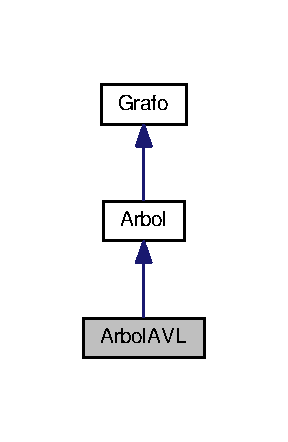
\includegraphics[width=138pt]{classArbolAVL__inherit__graph}
\end{center}
\end{figure}


Diagrama de colaboración para Arbol\+A\+VL\+:\nopagebreak
\begin{figure}[H]
\begin{center}
\leavevmode
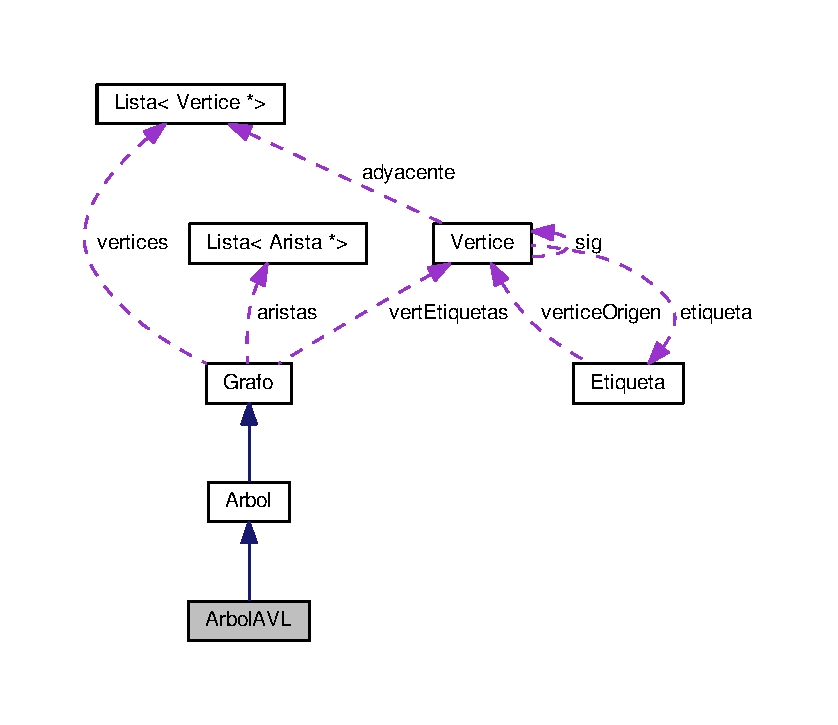
\includegraphics[width=350pt]{classArbolAVL__coll__graph}
\end{center}
\end{figure}
\subsection*{Métodos públicos}
\begin{DoxyCompactItemize}
\item 
\mbox{\Hypertarget{classArbolAVL_afd1b81c0fb7bd76fc8b924f15ca7e926}\label{classArbolAVL_afd1b81c0fb7bd76fc8b924f15ca7e926}} 
\hyperlink{classArbolAVL_afd1b81c0fb7bd76fc8b924f15ca7e926}{Arbol\+A\+VL} ()
\begin{DoxyCompactList}\small\item\em Consturctor de \hyperlink{classArbolAVL}{Arbol\+A\+VL}. \end{DoxyCompactList}\item 
void \hyperlink{classArbolAVL_a99512878bc14c77bf31ab7bf8dd6aa36}{insertar} (int dato)
\begin{DoxyCompactList}\small\item\em Inserta un dato en el árbol. \end{DoxyCompactList}\item 
void \hyperlink{classArbolAVL_ac88b4af2e6b96775793a981baba0763a}{\+\_\+\+\_\+insertar\+\_\+\+\_\+} (\hyperlink{classVertice}{Vertice} $\ast$raiz, \hyperlink{classVertice}{Vertice} $\ast$nuevo)
\begin{DoxyCompactList}\small\item\em Método recursivo para insertar un dato en el árbol. \end{DoxyCompactList}\item 
void \hyperlink{classArbolAVL_a498e8df16b6814ea1dad6bcdf274dc3f}{rotacion\+\_\+derecha} (\hyperlink{classVertice}{Vertice} $\ast$raiz)
\begin{DoxyCompactList}\small\item\em Método preliminar para realizar la rotación derecha. Verifica que la raiz dada exista y que tenga un hijo derecho. \end{DoxyCompactList}\item 
void \hyperlink{classArbolAVL_aedfb7658eb4f826aeba3fb98f50483e6}{rotacion\+\_\+izquierda} (\hyperlink{classVertice}{Vertice} $\ast$raiz)
\begin{DoxyCompactList}\small\item\em Método preliminar para realizar la rotación izquierda. Verifica que la raiz dada exista y que tenga un hijo izquierdo. \end{DoxyCompactList}\item 
void \hyperlink{classArbolAVL_a33dfba0b6e53caa0f2e4b71a8d2c6a7e}{rotacion\+\_\+derecha} (\hyperlink{classVertice}{Vertice} $\ast$raiz, \hyperlink{classVertice}{Vertice} $\ast$hijo\+Der)
\begin{DoxyCompactList}\small\item\em Realiza la rotación derecha. \end{DoxyCompactList}\item 
void \hyperlink{classArbolAVL_abfaf2247b607b040e328391ec8621546}{rotacion\+\_\+izquierda} (\hyperlink{classVertice}{Vertice} $\ast$raiz, \hyperlink{classVertice}{Vertice} $\ast$hijo\+Izq)
\begin{DoxyCompactList}\small\item\em Realiza la rotación izquierda. \end{DoxyCompactList}\item 
void \hyperlink{classArbolAVL_a0b4342509dd935785b6f54924e06afea}{rotacion\+\_\+doble\+\_\+izquierda} (\hyperlink{classVertice}{Vertice} $\ast$raiz)
\begin{DoxyCompactList}\small\item\em Método preliminar para realizar la rotación doble izquierda. \end{DoxyCompactList}\item 
void \hyperlink{classArbolAVL_af75605601cca6de40f6e6f5b11bfce8e}{rotacion\+\_\+doble\+\_\+derecha} (\hyperlink{classVertice}{Vertice} $\ast$raiz)
\begin{DoxyCompactList}\small\item\em Método preliminar para realizar la rotación doble derecha. \end{DoxyCompactList}\item 
void \hyperlink{classArbolAVL_a3115c59bd2be761c530eeeb11a169700}{rotacion\+\_\+doble\+\_\+izquierda} (\hyperlink{classVertice}{Vertice} $\ast$raiz, \hyperlink{classVertice}{Vertice} $\ast$hijo\+Der)
\begin{DoxyCompactList}\small\item\em Realiza la rotación doble izquierda, que es una composición de dos rotaciones. \end{DoxyCompactList}\item 
void \hyperlink{classArbolAVL_aa481f6a1014b68159b1fe753b96bde62}{rotacion\+\_\+doble\+\_\+derecha} (\hyperlink{classVertice}{Vertice} $\ast$raiz, \hyperlink{classVertice}{Vertice} $\ast$hijo\+Izq)
\begin{DoxyCompactList}\small\item\em Realiza la rotación doble derecha, que es una composición de dos rotaciones. \end{DoxyCompactList}\item 
\mbox{\Hypertarget{classArbolAVL_ae47585dbdb912214f41eab88eb979e33}\label{classArbolAVL_ae47585dbdb912214f41eab88eb979e33}} 
void \hyperlink{classArbolAVL_ae47585dbdb912214f41eab88eb979e33}{borrar} ()
\begin{DoxyCompactList}\small\item\em Borra todos los vertices del árbol. {\bfseries Se recomienda su uso S\+O\+LO en caso de necesitar probar el funcionamiento de la clase} \end{DoxyCompactList}\item 
void \hyperlink{classArbolAVL_a783a3ffe994d8c2b4069d2fd45afab7f}{test} ()
\begin{DoxyCompactList}\small\item\em Método que contiene ciertos valores ya definidos para probar el funcionamiento. {\bfseries Se recomienda su uso S\+O\+LO en caso de necesitar probar el funcionamiento de la clase} \end{DoxyCompactList}\item 
void \hyperlink{classArbolAVL_ae6341a610967afe9a45c6fcddb68c4c9}{factores\+\_\+de\+\_\+equilibrio} (\hyperlink{classVertice}{Vertice} $\ast$r)
\begin{DoxyCompactList}\small\item\em Mestra los factores de equilibrio de todos los vertices existentes actualmente en el subárbol dado. {\bfseries Se recomienda su uso S\+O\+LO en caso de necesitar probar el funcionamiento de la clase} \end{DoxyCompactList}\item 
void \hyperlink{classArbolAVL_aeb90eb1614513b7438f98a43766d573d}{test\+\_\+hardcore} (\hyperlink{classArbolAVL}{Arbol\+A\+VL} $\ast$a, int $\ast$vector, int n, bool por\+Pasos)
\begin{DoxyCompactList}\small\item\em Método que permite realizar las debidas pruebas del funcionamiento segun los valores dados a través del método \hyperlink{classArbolAVL_a783a3ffe994d8c2b4069d2fd45afab7f}{test()}. {\bfseries Se recomienda su uso S\+O\+LO en caso de necesitar probar el funcionamiento de la clase} \end{DoxyCompactList}\end{DoxyCompactItemize}
\subsection*{Métodos protegidos}
\begin{DoxyCompactItemize}
\item 
void \hyperlink{classArbolAVL_ad24ffafb198dac21a98ff19e8361fbd6}{equilibrar\+\_\+subarbol} (\hyperlink{classVertice}{Vertice} $\ast$raiz)
\begin{DoxyCompactList}\small\item\em Realiza las debidas comparaciones para determinar si el árbol requiere ser balanceado. \end{DoxyCompactList}\item 
int \hyperlink{classArbolAVL_a12f2ddd1c095720faf96b5685a94e13e}{factor\+\_\+de\+\_\+equilibrio} (\hyperlink{classVertice}{Vertice} $\ast$raiz)
\begin{DoxyCompactList}\small\item\em Obtiene el factor de equilibrio de la raíz dada. \end{DoxyCompactList}\item 
int \hyperlink{classArbolAVL_a8cf229fd1482232fbfe4803043eeec14}{factor\+\_\+de\+\_\+equilibrio} (\hyperlink{classVertice}{Vertice} $\ast$hijo\+Izq, \hyperlink{classVertice}{Vertice} $\ast$hijo\+Der)
\begin{DoxyCompactList}\small\item\em Obtiene el factor de equilibrio de la raíz en base a sus vértices hijo. \end{DoxyCompactList}\end{DoxyCompactItemize}
\subsection*{Otros miembros heredados}


\subsection{Descripción detallada}
Implementación de un arbol binario que por cada inserción se corrobore el balance del mismo y se pueda auto-\/balancear. 

Un Árbol A\+VL consiste en un árbol binario de búsqueda pero que cuenta con la cualidad de que siempre esta equilibrado. Esto último se debe a diferentes condiciones que se establecen para que el árbol se balancee en un momento determinado. ~\newline
 La condición principal para determinar si un árbol está balanceado es observar si su {\bfseries factor de equilibrio} $F_e = \{-1,0,1\}$ (para más detalle, véase \hyperlink{classArbolAVL_a8cf229fd1482232fbfe4803043eeec14}{factor\+\_\+de\+\_\+equilibrio(\+Vertice$\ast$, Vertice$\ast$)}). En caso de que no se cumpla con la condición mencionada anteriormente, se dice que el árbol está {\itshape desbalanceado}. ~\newline
 Cuando se busca balancear el árbol, se utiliza alguna de las rotaciones siguientes\+:
\begin{DoxyItemize}
\item Rotación simple izquierda (\hyperlink{classArbolAVL_abfaf2247b607b040e328391ec8621546}{rotacion\+\_\+izquierda(\+Vertice$\ast$, Vertice$\ast$)})
\item Rotación simple derecha (\hyperlink{classArbolAVL_a33dfba0b6e53caa0f2e4b71a8d2c6a7e}{rotacion\+\_\+derecha(\+Vertice$\ast$, Vertice$\ast$)})
\item Rotación doble izquierda (\hyperlink{classArbolAVL_a3115c59bd2be761c530eeeb11a169700}{rotacion\+\_\+doble\+\_\+izquierda(\+Vertice$\ast$, Vertice$\ast$)})
\item Rotación doble derecha (\hyperlink{classArbolAVL_aa481f6a1014b68159b1fe753b96bde62}{rotacion\+\_\+doble\+\_\+derecha(\+Vertice$\ast$, Vertice$\ast$)})
\end{DoxyItemize}

Véase \hyperlink{classArbolAVL_ad24ffafb198dac21a98ff19e8361fbd6}{equilibrar\+\_\+subarbol(\+Vertice$\ast$)} para saber el momento en el que se aplica una de las 4 rotaciones dadas. \begin{DoxySeeAlso}{Ver también}
\hyperlink{classArbolAVL_a8cf229fd1482232fbfe4803043eeec14}{factor\+\_\+de\+\_\+equilibrio(\+Vertice$\ast$, Vertice$\ast$)} 

\hyperlink{classArbolAVL_ad24ffafb198dac21a98ff19e8361fbd6}{equilibrar\+\_\+subarbol(\+Vertice$\ast$)} 
\end{DoxySeeAlso}


Definición en la línea 70 del archivo arbol\+A\+V\+L.\+hpp.



\subsection{Documentación de las funciones miembro}
\mbox{\Hypertarget{classArbolAVL_ac88b4af2e6b96775793a981baba0763a}\label{classArbolAVL_ac88b4af2e6b96775793a981baba0763a}} 
\index{Arbol\+A\+VL@{Arbol\+A\+VL}!\+\_\+\+\_\+insertar\+\_\+\+\_\+@{\+\_\+\+\_\+insertar\+\_\+\+\_\+}}
\index{\+\_\+\+\_\+insertar\+\_\+\+\_\+@{\+\_\+\+\_\+insertar\+\_\+\+\_\+}!Arbol\+A\+VL@{Arbol\+A\+VL}}
\subsubsection{\texorpdfstring{\+\_\+\+\_\+insertar\+\_\+\+\_\+()}{\_\_insertar\_\_()}}
{\footnotesize\ttfamily void Arbol\+A\+V\+L\+::\+\_\+\+\_\+insertar\+\_\+\+\_\+ (\begin{DoxyParamCaption}\item[{\hyperlink{classVertice}{Vertice} $\ast$}]{raiz,  }\item[{\hyperlink{classVertice}{Vertice} $\ast$}]{nuevo }\end{DoxyParamCaption})}



Método recursivo para insertar un dato en el árbol. 

Inserta el vertice de la forma en que usualmente debería hacerse, buscando si el valor de dicho vertice es menor o mayor o igual al vertice \char`\"{}subraíz\char`\"{} en el que se encuentra. De ahí que se inserte en la izquierda/derecha, o bien, se busque en el subárbol izquierdo/derecho hasta encontrar un lugar vacío. ~\newline
 Al final de realizar la inserción del vértice, se ejecuta la función \hyperlink{classArbolAVL_ad24ffafb198dac21a98ff19e8361fbd6}{equilibrar\+\_\+subarbol(\+Vertice$\ast$)}. Esta realmente es la única diferencia con el método de insertar entre los árboles normales y los árboles A\+VL.

Dentro de \hyperlink{classArbolAVL_ad24ffafb198dac21a98ff19e8361fbd6}{equilibrar\+\_\+subarbol(\+Vertice$\ast$)} se comparan factores de equilibrio de los vértices del subárbol que solamente están contenidos en el {\itshape camino} que empieza con el vértice raíz y termina con el nuevo vértice insertado. Ejemplo. Supóngase el siguiente árbol ~\newline
  ~\newline
 Si suponemos que el vértice $d$ es el último se ha ingresado, entonces las comparaciones se harían en el siguiente orden\+:
\begin{DoxyItemize}
\item Se equilibra el subárbol con raíz $b$
\item Se equilibra el subárbol con raíz $a$
\end{DoxyItemize}

Nótese que, como tal, no existe un camino del vértice $b$ al vértice $a$, ya que estamos hablando de que los árboles son {\itshape digrafos}. En este caso si existe una relación \{padre -\/$>$ hijo\} pero no una relación \{hijo -\/$>$ padre\}. Sin embargo, gracias a la recusrividad, es posible \char`\"{}seguir\char`\"{} este camino desde el vértice hijo hasta el vértice raíz. 
\begin{DoxyParams}{Parámetros}
{\em raiz} & puntero al vertice raiz del subárbol especificado \\
\hline
{\em nuevo} & puntero al vertice nuevo que se busca insertar \\
\hline
\end{DoxyParams}
\begin{DoxySeeAlso}{Ver también}
\hyperlink{classArbolAVL_ad24ffafb198dac21a98ff19e8361fbd6}{equilibrar\+\_\+subarbol(\+Vertice$\ast$)} 
\end{DoxySeeAlso}


Definición en la línea 555 del archivo arbol\+A\+V\+L.\+hpp.

\mbox{\Hypertarget{classArbolAVL_ad24ffafb198dac21a98ff19e8361fbd6}\label{classArbolAVL_ad24ffafb198dac21a98ff19e8361fbd6}} 
\index{Arbol\+A\+VL@{Arbol\+A\+VL}!equilibrar\+\_\+subarbol@{equilibrar\+\_\+subarbol}}
\index{equilibrar\+\_\+subarbol@{equilibrar\+\_\+subarbol}!Arbol\+A\+VL@{Arbol\+A\+VL}}
\subsubsection{\texorpdfstring{equilibrar\+\_\+subarbol()}{equilibrar\_subarbol()}}
{\footnotesize\ttfamily void Arbol\+A\+V\+L\+::equilibrar\+\_\+subarbol (\begin{DoxyParamCaption}\item[{\hyperlink{classVertice}{Vertice} $\ast$}]{raiz }\end{DoxyParamCaption})\hspace{0.3cm}{\ttfamily [protected]}}



Realiza las debidas comparaciones para determinar si el árbol requiere ser balanceado. 

Este método, según los siguientes criterios, ejecutará las rotaciones especificadas en Arboles\+A\+VL. Sean R un vértice raíz de un subárbol, I el hijo izquierdo de la raíz y D el hijo derecho de la raíz. Tenemos\+:
\begin{DoxyItemize}
\item Si $F_e(R) = -2$ y $F_e(I) = -1$, entonces se realizará la rotación izquierda (Véase \hyperlink{classArbolAVL_abfaf2247b607b040e328391ec8621546}{rotacion\+\_\+izquierda(\+Vertice$\ast$, Vertice$\ast$)})
\item Si $F_e(R) = 2$ y $F_e(D) = 1$, entonces se realizará la rotación derecha (Véase \hyperlink{classArbolAVL_a33dfba0b6e53caa0f2e4b71a8d2c6a7e}{rotacion\+\_\+derecha(\+Vertice$\ast$, Vertice$\ast$)})
\item Si $F_e(R) = 2$ y $F_e(D) = -1$, entonces se realizará la rotación doble izquierda (Véase \hyperlink{classArbolAVL_a3115c59bd2be761c530eeeb11a169700}{rotacion\+\_\+doble\+\_\+izquierda(\+Vertice$\ast$, Vertice$\ast$)})
\item Si $F_e(R) = -2$ y $F_e(I) = 1$, entonces se realizará la rotación doble derecha (Véase \hyperlink{classArbolAVL_aa481f6a1014b68159b1fe753b96bde62}{rotacion\+\_\+doble\+\_\+derecha(\+Vertice$\ast$, Vertice$\ast$)}) 
\begin{DoxyParams}{Parámetros}
{\em raiz} & puntero al vertice raíz del subárbol especificado \\
\hline
\end{DoxyParams}

\end{DoxyItemize}

Definición en la línea 572 del archivo arbol\+A\+V\+L.\+hpp.

\mbox{\Hypertarget{classArbolAVL_a12f2ddd1c095720faf96b5685a94e13e}\label{classArbolAVL_a12f2ddd1c095720faf96b5685a94e13e}} 
\index{Arbol\+A\+VL@{Arbol\+A\+VL}!factor\+\_\+de\+\_\+equilibrio@{factor\+\_\+de\+\_\+equilibrio}}
\index{factor\+\_\+de\+\_\+equilibrio@{factor\+\_\+de\+\_\+equilibrio}!Arbol\+A\+VL@{Arbol\+A\+VL}}
\subsubsection{\texorpdfstring{factor\+\_\+de\+\_\+equilibrio()}{factor\_de\_equilibrio()}\hspace{0.1cm}{\footnotesize\ttfamily [1/2]}}
{\footnotesize\ttfamily int Arbol\+A\+V\+L\+::factor\+\_\+de\+\_\+equilibrio (\begin{DoxyParamCaption}\item[{\hyperlink{classVertice}{Vertice} $\ast$}]{raiz }\end{DoxyParamCaption})\hspace{0.3cm}{\ttfamily [protected]}}



Obtiene el factor de equilibrio de la raíz dada. 

Comprueba que la raiz dada exista y que luego compara la altura de su hijo derecho y de su hijo izquierdo para determinar cual es factor de equilibrio de la raiz. Véase la función \hyperlink{classArbolAVL_a8cf229fd1482232fbfe4803043eeec14}{factor\+\_\+de\+\_\+equilibrio(\+Vertice$\ast$, Vertice$\ast$)} para entender el funcionamiento detallado 
\begin{DoxyParams}{Parámetros}
{\em raiz} & puntero al vertice raíz del subárbol especificado \\
\hline
\end{DoxyParams}
\begin{DoxyReturn}{Devuelve}
valor numérico referente al factor de equilibrio de la raiz 
\end{DoxyReturn}
\begin{DoxySeeAlso}{Ver también}
\hyperlink{classArbolAVL_a8cf229fd1482232fbfe4803043eeec14}{factor\+\_\+de\+\_\+equilibrio(\+Vertice$\ast$, Vertice$\ast$)} 
\end{DoxySeeAlso}


Definición en la línea 600 del archivo arbol\+A\+V\+L.\+hpp.

\mbox{\Hypertarget{classArbolAVL_a8cf229fd1482232fbfe4803043eeec14}\label{classArbolAVL_a8cf229fd1482232fbfe4803043eeec14}} 
\index{Arbol\+A\+VL@{Arbol\+A\+VL}!factor\+\_\+de\+\_\+equilibrio@{factor\+\_\+de\+\_\+equilibrio}}
\index{factor\+\_\+de\+\_\+equilibrio@{factor\+\_\+de\+\_\+equilibrio}!Arbol\+A\+VL@{Arbol\+A\+VL}}
\subsubsection{\texorpdfstring{factor\+\_\+de\+\_\+equilibrio()}{factor\_de\_equilibrio()}\hspace{0.1cm}{\footnotesize\ttfamily [2/2]}}
{\footnotesize\ttfamily int Arbol\+A\+V\+L\+::factor\+\_\+de\+\_\+equilibrio (\begin{DoxyParamCaption}\item[{\hyperlink{classVertice}{Vertice} $\ast$}]{hijo\+Izq,  }\item[{\hyperlink{classVertice}{Vertice} $\ast$}]{hijo\+Der }\end{DoxyParamCaption})\hspace{0.3cm}{\ttfamily [protected]}}



Obtiene el factor de equilibrio de la raíz en base a sus vértices hijo. 

Calcula el factor de equilibrio de la raiz en base a lo siguiente. Dados los vértices $R$, $D$ e $I$ el vértice raíz, el hijo derecho de la raiz y el hijo izquierdo de la raiz respectivamente, tenemos que \[ F_e(R) = altura(D) - altura(I) \] Donde $F_e$ es el {\itshape factor de equilibrio} de la raiz 
\begin{DoxyParams}{Parámetros}
{\em hijo\+Izq} & puntero al hijo izquierdo de la raiz dada \\
\hline
{\em hijo\+Der} & puntero al hijo derecho de la raiz dada \\
\hline
\end{DoxyParams}
\begin{DoxyReturn}{Devuelve}
valor numérico referente al factor de equilibrio de la raiz 
\end{DoxyReturn}


Definición en la línea 608 del archivo arbol\+A\+V\+L.\+hpp.

\mbox{\Hypertarget{classArbolAVL_ae6341a610967afe9a45c6fcddb68c4c9}\label{classArbolAVL_ae6341a610967afe9a45c6fcddb68c4c9}} 
\index{Arbol\+A\+VL@{Arbol\+A\+VL}!factores\+\_\+de\+\_\+equilibrio@{factores\+\_\+de\+\_\+equilibrio}}
\index{factores\+\_\+de\+\_\+equilibrio@{factores\+\_\+de\+\_\+equilibrio}!Arbol\+A\+VL@{Arbol\+A\+VL}}
\subsubsection{\texorpdfstring{factores\+\_\+de\+\_\+equilibrio()}{factores\_de\_equilibrio()}}
{\footnotesize\ttfamily void Arbol\+A\+V\+L\+::factores\+\_\+de\+\_\+equilibrio (\begin{DoxyParamCaption}\item[{\hyperlink{classVertice}{Vertice} $\ast$}]{r }\end{DoxyParamCaption})}



Mestra los factores de equilibrio de todos los vertices existentes actualmente en el subárbol dado. {\bfseries Se recomienda su uso S\+O\+LO en caso de necesitar probar el funcionamiento de la clase} 


\begin{DoxyParams}{Parámetros}
{\em r} & puntero al vertice raíz de dicho subárbol \\
\hline
\end{DoxyParams}
\begin{DoxySeeAlso}{Ver también}
\hyperlink{classArbolAVL_a8cf229fd1482232fbfe4803043eeec14}{factor\+\_\+de\+\_\+equilibrio(\+Vertice$\ast$, Vertice$\ast$)} 
\end{DoxySeeAlso}


Definición en la línea 332 del archivo arbol\+A\+V\+L.\+hpp.

\mbox{\Hypertarget{classArbolAVL_a99512878bc14c77bf31ab7bf8dd6aa36}\label{classArbolAVL_a99512878bc14c77bf31ab7bf8dd6aa36}} 
\index{Arbol\+A\+VL@{Arbol\+A\+VL}!insertar@{insertar}}
\index{insertar@{insertar}!Arbol\+A\+VL@{Arbol\+A\+VL}}
\subsubsection{\texorpdfstring{insertar()}{insertar()}}
{\footnotesize\ttfamily void Arbol\+A\+V\+L\+::insertar (\begin{DoxyParamCaption}\item[{int}]{dato }\end{DoxyParamCaption})}



Inserta un dato en el árbol. 

Determina si el árbol cuenta con cero o más vertices. En caso de no tener vértices, simplemente inserta el vértice como si fuera la raiz, y termina su ejecución. En caso contrario, llama a la función recursiva \char`\"{}\+\_\+\+\_\+insertar\+\_\+\+\_\+(\+Vertice$\ast$, Vertice$\ast$)\char`\"{} para ser insertado entre los vértices preexistentes. 
\begin{DoxyParams}{Parámetros}
{\em dato} & valor numérico a insertar \\
\hline
\end{DoxyParams}
\begin{DoxySeeAlso}{Ver también}
\char`\"{}\+\_\+\+\_\+insertar\+\_\+\+\_\+(\+Vertice$\ast$, Vertice$\ast$)\char`\"{} 
\end{DoxySeeAlso}


Definición en la línea 548 del archivo arbol\+A\+V\+L.\+hpp.

\mbox{\Hypertarget{classArbolAVL_a498e8df16b6814ea1dad6bcdf274dc3f}\label{classArbolAVL_a498e8df16b6814ea1dad6bcdf274dc3f}} 
\index{Arbol\+A\+VL@{Arbol\+A\+VL}!rotacion\+\_\+derecha@{rotacion\+\_\+derecha}}
\index{rotacion\+\_\+derecha@{rotacion\+\_\+derecha}!Arbol\+A\+VL@{Arbol\+A\+VL}}
\subsubsection{\texorpdfstring{rotacion\+\_\+derecha()}{rotacion\_derecha()}\hspace{0.1cm}{\footnotesize\ttfamily [1/2]}}
{\footnotesize\ttfamily void Arbol\+A\+V\+L\+::rotacion\+\_\+derecha (\begin{DoxyParamCaption}\item[{\hyperlink{classVertice}{Vertice} $\ast$}]{raiz }\end{DoxyParamCaption})}



Método preliminar para realizar la rotación derecha. Verifica que la raiz dada exista y que tenga un hijo derecho. 

Dirigirse a \hyperlink{classArbolAVL_a33dfba0b6e53caa0f2e4b71a8d2c6a7e}{rotacion\+\_\+derecha(\+Vertice $\ast$, Vertice $\ast$)} para ver el funcionamiento detallado 
\begin{DoxyParams}{Parámetros}
{\em raiz} & puntero al vertice raiz del subárbol especificado \\
\hline
\end{DoxyParams}
\begin{DoxySeeAlso}{Ver también}
\hyperlink{classArbolAVL_a33dfba0b6e53caa0f2e4b71a8d2c6a7e}{rotacion\+\_\+derecha(\+Vertice $\ast$, Vertice $\ast$)} 
\end{DoxySeeAlso}


Definición en la línea 379 del archivo arbol\+A\+V\+L.\+hpp.

\mbox{\Hypertarget{classArbolAVL_a33dfba0b6e53caa0f2e4b71a8d2c6a7e}\label{classArbolAVL_a33dfba0b6e53caa0f2e4b71a8d2c6a7e}} 
\index{Arbol\+A\+VL@{Arbol\+A\+VL}!rotacion\+\_\+derecha@{rotacion\+\_\+derecha}}
\index{rotacion\+\_\+derecha@{rotacion\+\_\+derecha}!Arbol\+A\+VL@{Arbol\+A\+VL}}
\subsubsection{\texorpdfstring{rotacion\+\_\+derecha()}{rotacion\_derecha()}\hspace{0.1cm}{\footnotesize\ttfamily [2/2]}}
{\footnotesize\ttfamily void Arbol\+A\+V\+L\+::rotacion\+\_\+derecha (\begin{DoxyParamCaption}\item[{\hyperlink{classVertice}{Vertice} $\ast$}]{raiz,  }\item[{\hyperlink{classVertice}{Vertice} $\ast$}]{hijo\+Der }\end{DoxyParamCaption})}



Realiza la rotación derecha. 

Para la rotación derecha, se tienen que tomar los siguientes datos. Dados un vertice $R$, raiz del subárbol en estudio y un vertice $X$, hijo derecho de la raiz, tenemos
\begin{DoxyItemize}
\item El hijo izquierdo de $X$ ahora será el hijo derecho de $R$
\item El vertice $X$ ahora será padre del vértice $R$, y $R$ será su hijo izquierdo ~\newline
  
\begin{DoxyParams}{Parámetros}
{\em raiz} & puntero al vertice raiz del subárbol especificado \\
\hline
{\em hijo\+Der} & puntero al vertice del hijo derecho de la raiz dada \\
\hline
\end{DoxyParams}

\end{DoxyItemize}

Definición en la línea 391 del archivo arbol\+A\+V\+L.\+hpp.

\mbox{\Hypertarget{classArbolAVL_af75605601cca6de40f6e6f5b11bfce8e}\label{classArbolAVL_af75605601cca6de40f6e6f5b11bfce8e}} 
\index{Arbol\+A\+VL@{Arbol\+A\+VL}!rotacion\+\_\+doble\+\_\+derecha@{rotacion\+\_\+doble\+\_\+derecha}}
\index{rotacion\+\_\+doble\+\_\+derecha@{rotacion\+\_\+doble\+\_\+derecha}!Arbol\+A\+VL@{Arbol\+A\+VL}}
\subsubsection{\texorpdfstring{rotacion\+\_\+doble\+\_\+derecha()}{rotacion\_doble\_derecha()}\hspace{0.1cm}{\footnotesize\ttfamily [1/2]}}
{\footnotesize\ttfamily void Arbol\+A\+V\+L\+::rotacion\+\_\+doble\+\_\+derecha (\begin{DoxyParamCaption}\item[{\hyperlink{classVertice}{Vertice} $\ast$}]{raiz }\end{DoxyParamCaption})}



Método preliminar para realizar la rotación doble derecha. 

Dirigirse a \hyperlink{classArbolAVL_aa481f6a1014b68159b1fe753b96bde62}{rotacion\+\_\+doble\+\_\+derecha(\+Vertice $\ast$, Vertice $\ast$)} para ver el funcionamiento detallado 
\begin{DoxyParams}{Parámetros}
{\em raiz} & puntero al vertice raiz del subárbol especificado \\
\hline
\end{DoxyParams}
\begin{DoxySeeAlso}{Ver también}
\hyperlink{classArbolAVL_aa481f6a1014b68159b1fe753b96bde62}{rotacion\+\_\+doble\+\_\+derecha(\+Vertice $\ast$, Vertice $\ast$)} 
\end{DoxySeeAlso}


Definición en la línea 494 del archivo arbol\+A\+V\+L.\+hpp.

\mbox{\Hypertarget{classArbolAVL_aa481f6a1014b68159b1fe753b96bde62}\label{classArbolAVL_aa481f6a1014b68159b1fe753b96bde62}} 
\index{Arbol\+A\+VL@{Arbol\+A\+VL}!rotacion\+\_\+doble\+\_\+derecha@{rotacion\+\_\+doble\+\_\+derecha}}
\index{rotacion\+\_\+doble\+\_\+derecha@{rotacion\+\_\+doble\+\_\+derecha}!Arbol\+A\+VL@{Arbol\+A\+VL}}
\subsubsection{\texorpdfstring{rotacion\+\_\+doble\+\_\+derecha()}{rotacion\_doble\_derecha()}\hspace{0.1cm}{\footnotesize\ttfamily [2/2]}}
{\footnotesize\ttfamily void Arbol\+A\+V\+L\+::rotacion\+\_\+doble\+\_\+derecha (\begin{DoxyParamCaption}\item[{\hyperlink{classVertice}{Vertice} $\ast$}]{raiz,  }\item[{\hyperlink{classVertice}{Vertice} $\ast$}]{hijo\+Izq }\end{DoxyParamCaption})}



Realiza la rotación doble derecha, que es una composición de dos rotaciones. 

Este método realiza la rotación doble derecha la cual consiste en\+:
\begin{DoxyItemize}
\item realizar una rotación derecha en el hijo izquierdo de la raiz
\item realizar una rotación izquierda en la raiz del subárbol
\end{DoxyItemize}

Dados un vértice R raíz de todo el subárbol y un vértice X hijo izquierdo de la raíz. Se tiene la siguiente ilustración ~\newline
  
\begin{DoxyParams}{Parámetros}
{\em raiz} & puntero al vertice raiz del subárbol especificado \\
\hline
{\em hijo\+Izq} & puntero al vertice del hijo izquierdo de la raiz dada \\
\hline
\end{DoxyParams}


Definición en la línea 508 del archivo arbol\+A\+V\+L.\+hpp.

\mbox{\Hypertarget{classArbolAVL_a0b4342509dd935785b6f54924e06afea}\label{classArbolAVL_a0b4342509dd935785b6f54924e06afea}} 
\index{Arbol\+A\+VL@{Arbol\+A\+VL}!rotacion\+\_\+doble\+\_\+izquierda@{rotacion\+\_\+doble\+\_\+izquierda}}
\index{rotacion\+\_\+doble\+\_\+izquierda@{rotacion\+\_\+doble\+\_\+izquierda}!Arbol\+A\+VL@{Arbol\+A\+VL}}
\subsubsection{\texorpdfstring{rotacion\+\_\+doble\+\_\+izquierda()}{rotacion\_doble\_izquierda()}\hspace{0.1cm}{\footnotesize\ttfamily [1/2]}}
{\footnotesize\ttfamily void Arbol\+A\+V\+L\+::rotacion\+\_\+doble\+\_\+izquierda (\begin{DoxyParamCaption}\item[{\hyperlink{classVertice}{Vertice} $\ast$}]{raiz }\end{DoxyParamCaption})}



Método preliminar para realizar la rotación doble izquierda. 

Dirigirse a \hyperlink{classArbolAVL_a3115c59bd2be761c530eeeb11a169700}{rotacion\+\_\+doble\+\_\+izquierda(\+Vertice $\ast$, Vertice $\ast$)} para ver el funcionamiento detallado 
\begin{DoxyParams}{Parámetros}
{\em raiz} & puntero al vertice raiz del subárbol especificado \\
\hline
\end{DoxyParams}
\begin{DoxySeeAlso}{Ver también}
\hyperlink{classArbolAVL_a3115c59bd2be761c530eeeb11a169700}{rotacion\+\_\+doble\+\_\+izquierda(\+Vertice $\ast$, Vertice $\ast$)} 
\end{DoxySeeAlso}


Definición en la línea 499 del archivo arbol\+A\+V\+L.\+hpp.

\mbox{\Hypertarget{classArbolAVL_a3115c59bd2be761c530eeeb11a169700}\label{classArbolAVL_a3115c59bd2be761c530eeeb11a169700}} 
\index{Arbol\+A\+VL@{Arbol\+A\+VL}!rotacion\+\_\+doble\+\_\+izquierda@{rotacion\+\_\+doble\+\_\+izquierda}}
\index{rotacion\+\_\+doble\+\_\+izquierda@{rotacion\+\_\+doble\+\_\+izquierda}!Arbol\+A\+VL@{Arbol\+A\+VL}}
\subsubsection{\texorpdfstring{rotacion\+\_\+doble\+\_\+izquierda()}{rotacion\_doble\_izquierda()}\hspace{0.1cm}{\footnotesize\ttfamily [2/2]}}
{\footnotesize\ttfamily void Arbol\+A\+V\+L\+::rotacion\+\_\+doble\+\_\+izquierda (\begin{DoxyParamCaption}\item[{\hyperlink{classVertice}{Vertice} $\ast$}]{raiz,  }\item[{\hyperlink{classVertice}{Vertice} $\ast$}]{hijo\+Der }\end{DoxyParamCaption})}



Realiza la rotación doble izquierda, que es una composición de dos rotaciones. 

Este método realiza la rotación doble izquierda la cual consiste en\+:
\begin{DoxyItemize}
\item realizar una rotación izquierda en el hijo derecho de la raiz
\item realizar una rotación derecha en la raiz del subárbol
\end{DoxyItemize}

Dados un vértice R raíz de todo el subárbol y un vértice X hijo derecho de la raíz. Se tiene la siguiente ilustración ~\newline
  
\begin{DoxyParams}{Parámetros}
{\em raiz} & puntero al vertice raiz del subárbol especificado \\
\hline
{\em hijo\+Der} & puntero al vertice del hijo derecho de la raiz dada \\
\hline
\end{DoxyParams}


Definición en la línea 530 del archivo arbol\+A\+V\+L.\+hpp.

\mbox{\Hypertarget{classArbolAVL_aedfb7658eb4f826aeba3fb98f50483e6}\label{classArbolAVL_aedfb7658eb4f826aeba3fb98f50483e6}} 
\index{Arbol\+A\+VL@{Arbol\+A\+VL}!rotacion\+\_\+izquierda@{rotacion\+\_\+izquierda}}
\index{rotacion\+\_\+izquierda@{rotacion\+\_\+izquierda}!Arbol\+A\+VL@{Arbol\+A\+VL}}
\subsubsection{\texorpdfstring{rotacion\+\_\+izquierda()}{rotacion\_izquierda()}\hspace{0.1cm}{\footnotesize\ttfamily [1/2]}}
{\footnotesize\ttfamily void Arbol\+A\+V\+L\+::rotacion\+\_\+izquierda (\begin{DoxyParamCaption}\item[{\hyperlink{classVertice}{Vertice} $\ast$}]{raiz }\end{DoxyParamCaption})}



Método preliminar para realizar la rotación izquierda. Verifica que la raiz dada exista y que tenga un hijo izquierdo. 

Dirigirse a \hyperlink{classArbolAVL_abfaf2247b607b040e328391ec8621546}{rotacion\+\_\+izquierda(\+Vertice $\ast$, Vertice $\ast$)} para ver el funcionamiento detallado 
\begin{DoxyParams}{Parámetros}
{\em raiz} & puntero al vertice raiz del subárbol especificado \\
\hline
\end{DoxyParams}
\begin{DoxySeeAlso}{Ver también}
\hyperlink{classArbolAVL_abfaf2247b607b040e328391ec8621546}{rotacion\+\_\+izquierda(\+Vertice $\ast$, Vertice $\ast$)} 
\end{DoxySeeAlso}


Definición en la línea 437 del archivo arbol\+A\+V\+L.\+hpp.

\mbox{\Hypertarget{classArbolAVL_abfaf2247b607b040e328391ec8621546}\label{classArbolAVL_abfaf2247b607b040e328391ec8621546}} 
\index{Arbol\+A\+VL@{Arbol\+A\+VL}!rotacion\+\_\+izquierda@{rotacion\+\_\+izquierda}}
\index{rotacion\+\_\+izquierda@{rotacion\+\_\+izquierda}!Arbol\+A\+VL@{Arbol\+A\+VL}}
\subsubsection{\texorpdfstring{rotacion\+\_\+izquierda()}{rotacion\_izquierda()}\hspace{0.1cm}{\footnotesize\ttfamily [2/2]}}
{\footnotesize\ttfamily void Arbol\+A\+V\+L\+::rotacion\+\_\+izquierda (\begin{DoxyParamCaption}\item[{\hyperlink{classVertice}{Vertice} $\ast$}]{raiz,  }\item[{\hyperlink{classVertice}{Vertice} $\ast$}]{hijo\+Izq }\end{DoxyParamCaption})}



Realiza la rotación izquierda. 

Para la rotación izquierda, se tienen que tomar los siguientes datos. Dados un vertice $R$, raiz del subárbol en estudio y un vertice $X$, hijo izquierdo de la raiz, tenemos
\begin{DoxyItemize}
\item El hijo derecho de $X$ ahora será el hijo izquierdo de $R$
\item El vertice $X$ ahora será padre del vértice $R$, y $R$ será su hijo derecho ~\newline
  
\begin{DoxyParams}{Parámetros}
{\em raiz} & puntero al vertice raiz del subárbol especificado \\
\hline
{\em hijo\+Izq} & puntero al vertice del hijo izquierdo de la raiz dada \\
\hline
\end{DoxyParams}

\end{DoxyItemize}

Definición en la línea 449 del archivo arbol\+A\+V\+L.\+hpp.

\mbox{\Hypertarget{classArbolAVL_a783a3ffe994d8c2b4069d2fd45afab7f}\label{classArbolAVL_a783a3ffe994d8c2b4069d2fd45afab7f}} 
\index{Arbol\+A\+VL@{Arbol\+A\+VL}!test@{test}}
\index{test@{test}!Arbol\+A\+VL@{Arbol\+A\+VL}}
\subsubsection{\texorpdfstring{test()}{test()}}
{\footnotesize\ttfamily void Arbol\+A\+V\+L\+::test (\begin{DoxyParamCaption}{ }\end{DoxyParamCaption})}



Método que contiene ciertos valores ya definidos para probar el funcionamiento. {\bfseries Se recomienda su uso S\+O\+LO en caso de necesitar probar el funcionamiento de la clase} 

\begin{DoxySeeAlso}{Ver también}
\hyperlink{classArbolAVL_aeb90eb1614513b7438f98a43766d573d}{test\+\_\+hardcore(\+Arbol\+A\+V\+L$\ast$, int$\ast$, int, bool)} 
\end{DoxySeeAlso}


Definición en la línea 361 del archivo arbol\+A\+V\+L.\+hpp.

\mbox{\Hypertarget{classArbolAVL_aeb90eb1614513b7438f98a43766d573d}\label{classArbolAVL_aeb90eb1614513b7438f98a43766d573d}} 
\index{Arbol\+A\+VL@{Arbol\+A\+VL}!test\+\_\+hardcore@{test\+\_\+hardcore}}
\index{test\+\_\+hardcore@{test\+\_\+hardcore}!Arbol\+A\+VL@{Arbol\+A\+VL}}
\subsubsection{\texorpdfstring{test\+\_\+hardcore()}{test\_hardcore()}}
{\footnotesize\ttfamily void Arbol\+A\+V\+L\+::test\+\_\+hardcore (\begin{DoxyParamCaption}\item[{\hyperlink{classArbolAVL}{Arbol\+A\+VL} $\ast$}]{a,  }\item[{int $\ast$}]{vector,  }\item[{int}]{n,  }\item[{bool}]{por\+Pasos }\end{DoxyParamCaption})}



Método que permite realizar las debidas pruebas del funcionamiento segun los valores dados a través del método \hyperlink{classArbolAVL_a783a3ffe994d8c2b4069d2fd45afab7f}{test()}. {\bfseries Se recomienda su uso S\+O\+LO en caso de necesitar probar el funcionamiento de la clase} 


\begin{DoxyParams}{Parámetros}
{\em a} & puntero a un \hyperlink{classArbolAVL}{Arbol\+A\+VL} \\
\hline
{\em vector} & arreglo de valores numericos de cada vertice \\
\hline
{\em n} & cantidad de elementos en el arreglo \\
\hline
{\em por\+Pasos} & booleano que determina si mostrarán individualmente las inserciones o no. \\
\hline
\end{DoxyParams}
\begin{DoxySeeAlso}{Ver también}
\hyperlink{classArbolAVL_a783a3ffe994d8c2b4069d2fd45afab7f}{test()} 
\end{DoxySeeAlso}


Definición en la línea 342 del archivo arbol\+A\+V\+L.\+hpp.



La documentación para esta clase fue generada a partir del siguiente fichero\+:\begin{DoxyCompactItemize}
\item 
\hyperlink{arbolAVL_8hpp}{arbol\+A\+V\+L.\+hpp}\end{DoxyCompactItemize}

\hypertarget{classArista}{}\section{Referencia de la Clase Arista}
\label{classArista}\index{Arista@{Arista}}


Diagrama de colaboración para Arista\+:
% FIG 0
\subsection*{Métodos públicos}
\begin{DoxyCompactItemize}
\item 
\mbox{\Hypertarget{classArista_abfc5e334e70240f90b0f8d0cc094ad40}\label{classArista_abfc5e334e70240f90b0f8d0cc094ad40}} 
{\bfseries Arista} (\hyperlink{classVertice}{Vertice} $\ast$o, \hyperlink{classVertice}{Vertice} $\ast$d, float p)
\end{DoxyCompactItemize}
\subsection*{Atributos públicos}
\begin{DoxyCompactItemize}
\item 
\mbox{\Hypertarget{classArista_a9eb724ff0d46897de85b760d36a2e6b4}\label{classArista_a9eb724ff0d46897de85b760d36a2e6b4}} 
\hyperlink{classVertice}{Vertice} $\ast$ {\bfseries origen}
\item 
\mbox{\Hypertarget{classArista_a41f8fed9f49c9216330c65caafc145d1}\label{classArista_a41f8fed9f49c9216330c65caafc145d1}} 
\hyperlink{classVertice}{Vertice} $\ast$ {\bfseries destino}
\item 
\mbox{\Hypertarget{classArista_a371fdf684b589d3b3d842ad5ae338342}\label{classArista_a371fdf684b589d3b3d842ad5ae338342}} 
float {\bfseries peso}
\end{DoxyCompactItemize}


\subsection{Descripción detallada}


Definición en la línea 56 del archivo grafo.\+h.



La documentación para esta clase fue generada a partir del siguiente fichero\+:\begin{DoxyCompactItemize}
\item 
grafo.\+h\end{DoxyCompactItemize}

\hypertarget{classcola}{}\section{Referencia de la plantilla de la Clase cola$<$ T\+I\+PO $>$}
\label{classcola}\index{cola$<$ T\+I\+P\+O $>$@{cola$<$ T\+I\+P\+O $>$}}
\subsection*{Métodos públicos}
\begin{DoxyCompactItemize}
\item 
\mbox{\Hypertarget{classcola_a2af9a71dd856a907f446a1e396d83e5b}\label{classcola_a2af9a71dd856a907f446a1e396d83e5b}} 
bool {\bfseries vacio} ()
\item 
\mbox{\Hypertarget{classcola_a4fe29cbff3478979d38a0f8a2d7a4b51}\label{classcola_a4fe29cbff3478979d38a0f8a2d7a4b51}} 
void {\bfseries encolar} (T\+I\+PO v)
\item 
\mbox{\Hypertarget{classcola_afbe13fa4237aa2fde61067900ff8f884}\label{classcola_afbe13fa4237aa2fde61067900ff8f884}} 
T\+I\+PO {\bfseries desencolar} ()
\end{DoxyCompactItemize}


\subsection{Descripción detallada}
\subsubsection*{template$<$class T\+I\+PO$>$\newline
class cola$<$ T\+I\+P\+O $>$}



Definición en la línea 14 del archivo cola.\+h.



La documentación para esta clase fue generada a partir del siguiente fichero\+:\begin{DoxyCompactItemize}
\item 
cola.\+h\end{DoxyCompactItemize}

\hypertarget{classEtiqueta}{}\section{Referencia de la Clase Etiqueta}
\label{classEtiqueta}\index{Etiqueta@{Etiqueta}}


Diagrama de colaboración para Etiqueta\+:
% FIG 0
\subsection*{Métodos públicos}
\begin{DoxyCompactItemize}
\item 
\mbox{\Hypertarget{classEtiqueta_aa7f1cc55f5fed8f31cc176d375544349}\label{classEtiqueta_aa7f1cc55f5fed8f31cc176d375544349}} 
{\bfseries Etiqueta} (float p, \hyperlink{classVertice}{Vertice} $\ast$origen, bool permanente)
\end{DoxyCompactItemize}
\subsection*{Atributos públicos}
\begin{DoxyCompactItemize}
\item 
\mbox{\Hypertarget{classEtiqueta_a6cb53a3db11a5f79617642d5a3b1a2fa}\label{classEtiqueta_a6cb53a3db11a5f79617642d5a3b1a2fa}} 
float {\bfseries peso}
\item 
\mbox{\Hypertarget{classEtiqueta_abbc7c11fe50bd7ae2a34949e10e66fff}\label{classEtiqueta_abbc7c11fe50bd7ae2a34949e10e66fff}} 
\hyperlink{classVertice}{Vertice} $\ast$ {\bfseries vertice\+Origen}
\item 
\mbox{\Hypertarget{classEtiqueta_aa69958b23c24051acace2d464be55de4}\label{classEtiqueta_aa69958b23c24051acace2d464be55de4}} 
bool {\bfseries permanente}
\end{DoxyCompactItemize}


\subsection{Descripción detallada}


Definición en la línea 14 del archivo grafo.\+h.



La documentación para esta clase fue generada a partir del siguiente fichero\+:\begin{DoxyCompactItemize}
\item 
grafo.\+h\end{DoxyCompactItemize}

\hypertarget{classGrafo}{}\section{Referencia de la Clase Grafo}
\label{classGrafo}\index{Grafo@{Grafo}}


Diagrama de herencias de Grafo
% FIG 0


Diagrama de colaboración para Grafo\+:
% FIG 1
\subsection*{Métodos públicos}
\begin{DoxyCompactItemize}
\item 
\mbox{\Hypertarget{classGrafo_acffb2ecb4e945a429ee650ef86c50828}\label{classGrafo_acffb2ecb4e945a429ee650ef86c50828}} 
int {\bfseries cardinalidad} ()
\item 
\mbox{\Hypertarget{classGrafo_a1b0368926f9523063c42373e7b85f71f}\label{classGrafo_a1b0368926f9523063c42373e7b85f71f}} 
bool {\bfseries vacio} ()
\item 
\mbox{\Hypertarget{classGrafo_a7bfb0f93720820e9d0cb8091f32d69a7}\label{classGrafo_a7bfb0f93720820e9d0cb8091f32d69a7}} 
bool {\bfseries comprobar\+\_\+adyacencia} (string origen, string destino)
\item 
\mbox{\Hypertarget{classGrafo_ade13f10eecc05a5a08ef43c26b53e248}\label{classGrafo_ade13f10eecc05a5a08ef43c26b53e248}} 
bool {\bfseries insertar\+\_\+vertice} (string nombre)
\item 
\mbox{\Hypertarget{classGrafo_a45450097c4398a0539689245784adf4a}\label{classGrafo_a45450097c4398a0539689245784adf4a}} 
bool {\bfseries insertar\+\_\+vertice} (string nombre, int dato)
\item 
\mbox{\Hypertarget{classGrafo_ae49d7c6c60a6b5bb1a7e66ef72144d36}\label{classGrafo_ae49d7c6c60a6b5bb1a7e66ef72144d36}} 
void {\bfseries insertar\+\_\+arista} (\hyperlink{classVertice}{Vertice} $\ast$origen, \hyperlink{classVertice}{Vertice} $\ast$destino, float peso)
\item 
\mbox{\Hypertarget{classGrafo_a3d18ac8c9af95b06e7e17671b4d17b3c}\label{classGrafo_a3d18ac8c9af95b06e7e17671b4d17b3c}} 
void {\bfseries lista\+\_\+adyacencia} ()
\item 
\mbox{\Hypertarget{classGrafo_a1c65e0f7cbbf74cd690b5eddf220728d}\label{classGrafo_a1c65e0f7cbbf74cd690b5eddf220728d}} 
\hyperlink{classLista}{Lista}$<$ \hyperlink{classVertice}{Vertice} $\ast$ $>$ $\ast$ {\bfseries recorrido\+\_\+en\+\_\+anchura} (\hyperlink{classVertice}{Vertice} $\ast$origen)
\item 
\mbox{\Hypertarget{classGrafo_ae2773db77afaab3b02a8237b93091818}\label{classGrafo_ae2773db77afaab3b02a8237b93091818}} 
\hyperlink{classLista}{Lista}$<$ \hyperlink{classVertice}{Vertice} $\ast$ $>$ $\ast$ {\bfseries recorrido\+\_\+en\+\_\+profundidad} (\hyperlink{classVertice}{Vertice} $\ast$origen)
\item 
\mbox{\Hypertarget{classGrafo_ac088cffbe30ed4c895ac831233251d99}\label{classGrafo_ac088cffbe30ed4c895ac831233251d99}} 
\hyperlink{classVertice}{Vertice} $\ast$ {\bfseries get\+\_\+vertice} (string nombre)
\item 
\mbox{\Hypertarget{classGrafo_a4baa752c1e6a7e6367672581525c3c19}\label{classGrafo_a4baa752c1e6a7e6367672581525c3c19}} 
\hyperlink{classVertice}{Vertice} $\ast$ {\bfseries get\+\_\+vertice\+\_\+inicial} ()
\item 
\mbox{\Hypertarget{classGrafo_aed632e897451b00634e8f1d8088c12c8}\label{classGrafo_aed632e897451b00634e8f1d8088c12c8}} 
\hyperlink{classArista}{Arista} $\ast$ {\bfseries get\+\_\+arista} (\hyperlink{classVertice}{Vertice} $\ast$origen, \hyperlink{classVertice}{Vertice} $\ast$destino)
\item 
\mbox{\Hypertarget{classGrafo_a4bb5d2fe50503dd9f6c8042cee3e3631}\label{classGrafo_a4bb5d2fe50503dd9f6c8042cee3e3631}} 
\hyperlink{classLista}{Lista}$<$ \hyperlink{classVertice}{Vertice} $\ast$ $>$ $\ast$ {\bfseries dijkstra} (\hyperlink{classVertice}{Vertice} $\ast$origen, \hyperlink{classVertice}{Vertice} $\ast$destino)
\item 
\mbox{\Hypertarget{classGrafo_a50fe04d01b2d34b777d8df0b827bedab}\label{classGrafo_a50fe04d01b2d34b777d8df0b827bedab}} 
bool {\bfseries conexo} ()
\item 
\mbox{\Hypertarget{classGrafo_a40fa3c86b1e2890d4dad315bbd59d2d0}\label{classGrafo_a40fa3c86b1e2890d4dad315bbd59d2d0}} 
bool {\bfseries dirigido} ()
\item 
\mbox{\Hypertarget{classGrafo_aa2ab9a12d473f6830af554efad5b438d}\label{classGrafo_aa2ab9a12d473f6830af554efad5b438d}} 
\hyperlink{classGrafo}{Grafo} $\ast$ {\bfseries kruskal} ()
\item 
\mbox{\Hypertarget{classGrafo_a24cc1dad8b719978e5fcba8b0950c3f5}\label{classGrafo_a24cc1dad8b719978e5fcba8b0950c3f5}} 
bool {\bfseries hay\+\_\+camino} (\hyperlink{classVertice}{Vertice} $\ast$origen, \hyperlink{classVertice}{Vertice} $\ast$destino)
\end{DoxyCompactItemize}
\subsection*{Atributos protegidos}
\begin{DoxyCompactItemize}
\item 
\mbox{\Hypertarget{classGrafo_af6719d649fae513eb84ef8bf502c1812}\label{classGrafo_af6719d649fae513eb84ef8bf502c1812}} 
\hyperlink{classLista}{Lista}$<$ \hyperlink{classVertice}{Vertice} $\ast$ $>$ {\bfseries vertices}
\item 
\mbox{\Hypertarget{classGrafo_a69300beee0528e08e810d91b6f968d02}\label{classGrafo_a69300beee0528e08e810d91b6f968d02}} 
\hyperlink{classLista}{Lista}$<$ \hyperlink{classArista}{Arista} $\ast$ $>$ {\bfseries aristas}
\item 
\mbox{\Hypertarget{classGrafo_a67e71aebff46a360d82771b825f71263}\label{classGrafo_a67e71aebff46a360d82771b825f71263}} 
\hyperlink{classVertice}{Vertice} $\ast$ {\bfseries vert\+Etiquetas}
\end{DoxyCompactItemize}


\subsection{Descripción detallada}


Definición en la línea 65 del archivo grafo.\+h.



La documentación para esta clase fue generada a partir del siguiente fichero\+:\begin{DoxyCompactItemize}
\item 
grafo.\+h\end{DoxyCompactItemize}

\hypertarget{classLista_1_1iterator}{}\section{Referencia de la Clase Lista$<$ tipo $>$\+:\+:iterator}
\label{classLista_1_1iterator}\index{Lista$<$ tipo $>$\+::iterator@{Lista$<$ tipo $>$\+::iterator}}


Clase que ayuda a acceder a los elementos del T\+DA \hyperlink{classLista}{Lista}.  




{\ttfamily \#include $<$lista.\+hpp$>$}

\subsection*{Métodos públicos}
\begin{DoxyCompactItemize}
\item 
\hyperlink{classLista_1_1iterator_a1535d6055cf70a60518be63c0f62cc1d}{iterator} (\hyperlink{classLista}{Lista}$<$ tipo $>$ \&il)
\begin{DoxyCompactList}\small\item\em Constructor de la clase iterator para definir el inicio. \end{DoxyCompactList}\item 
\hyperlink{classLista_1_1iterator_ad96ff61e26fb131406d0b320b36e9516}{iterator} (\hyperlink{classLista}{Lista}$<$ tipo $>$ \&il, bool)
\begin{DoxyCompactList}\small\item\em Constructor de la clase iterator para definir el final. \end{DoxyCompactList}\item 
tipo \hyperlink{classLista_1_1iterator_af8c7d385ce8bc7c62b8bc806db714ae9}{operator++} ()
\begin{DoxyCompactList}\small\item\em Funcion para aumentar el indice iterador. \end{DoxyCompactList}\item 
tipo \hyperlink{classLista_1_1iterator_ac9059ed8e1f396ec967ae97b571d11fe}{operator++} (int)
\begin{DoxyCompactList}\small\item\em Funcion para aumentar el indice iterador. \end{DoxyCompactList}\item 
\hyperlink{classLista_1_1iterator}{iterator} \& \hyperlink{classLista_1_1iterator_a99315852e99d13cfac11f570917ac092}{operator+=} (int amount)
\begin{DoxyCompactList}\small\item\em Funcion para aumentar la cantidad predeterminada de elementos. \end{DoxyCompactList}\item 
\hyperlink{classLista_1_1iterator}{iterator} \& \hyperlink{classLista_1_1iterator_a602f51e54500d6027158a48a8495826a}{operator=} (const \hyperlink{classLista_1_1iterator}{iterator} \&aa)
\begin{DoxyCompactList}\small\item\em Funcion para ver si estas en el final de la lista / o comparar iteradores. \end{DoxyCompactList}\item 
tipo \& \hyperlink{classLista_1_1iterator_a2a48c3991820aef39d777df2c8e19664}{operator$\ast$} ()
\begin{DoxyCompactList}\small\item\em Funcion para obtener el valor del actual. \end{DoxyCompactList}\item 
bool \hyperlink{classLista_1_1iterator_abb50011145596234ea6ac6d1bd5fe920}{operator==} (const \hyperlink{classLista_1_1iterator}{iterator} \&rv) const
\begin{DoxyCompactList}\small\item\em Funcion para ver si estas en el final de la lista / o comparar iteradores. \end{DoxyCompactList}\item 
bool \hyperlink{classLista_1_1iterator_a25cd74ab23dd46dd3e9f0769c0264eb9}{operator!=} (const \hyperlink{classLista_1_1iterator}{iterator} \&rv) const
\begin{DoxyCompactList}\small\item\em Funcion para saber si el iterador es distinto de otro iterador ? \end{DoxyCompactList}\item 
tipo \hyperlink{classLista_1_1iterator_a6e73de7c83716c9bd99bd68b89214d81}{current} () const
\begin{DoxyCompactList}\small\item\em Funcion para obtener el elemento actual. \end{DoxyCompactList}\end{DoxyCompactItemize}
\subsection*{Amigas}
\begin{DoxyCompactItemize}
\item 
std\+::ostream \& \hyperlink{classLista_1_1iterator_ab86d5cacfaca06c9075ddb7427cf7ddb}{operator$<$$<$} (std\+::ostream \&os, const \hyperlink{classLista_1_1iterator}{iterator} \&it)
\begin{DoxyCompactList}\small\item\em Funcion para imprimir en pantalla. \end{DoxyCompactList}\end{DoxyCompactItemize}
\subsection*{Funciones relacionadas}
(Observar que estas no son funciones miembro.) \begin{DoxyCompactItemize}
\item 
\mbox{\Hypertarget{classLista_1_1iterator_a67171474c4da6cc8efe0c7fafefd2b2d}\label{classLista_1_1iterator_a67171474c4da6cc8efe0c7fafefd2b2d}} 
class \hyperlink{classLista_1_1iterator_a67171474c4da6cc8efe0c7fafefd2b2d}{iterator}
\begin{DoxyCompactList}\small\item\em iterador adicional. \end{DoxyCompactList}\end{DoxyCompactItemize}


\subsection{Descripción detallada}
\subsubsection*{template$<$typename tipo$>$\newline
class Lista$<$ tipo $>$\+::iterator}

Clase que ayuda a acceder a los elementos del T\+DA \hyperlink{classLista}{Lista}. 

Definición en la línea 182 del archivo lista.\+hpp.



\subsection{Documentación del constructor y destructor}
\mbox{\Hypertarget{classLista_1_1iterator_a1535d6055cf70a60518be63c0f62cc1d}\label{classLista_1_1iterator_a1535d6055cf70a60518be63c0f62cc1d}} 
\index{Lista\+::iterator@{Lista\+::iterator}!iterator@{iterator}}
\index{iterator@{iterator}!Lista\+::iterator@{Lista\+::iterator}}
\subsubsection{\texorpdfstring{iterator()}{iterator()}\hspace{0.1cm}{\footnotesize\ttfamily [1/2]}}
{\footnotesize\ttfamily template$<$typename tipo$>$ \\
\hyperlink{classLista}{Lista}$<$ tipo $>$\+::iterator\+::iterator (\begin{DoxyParamCaption}\item[{\hyperlink{classLista}{Lista}$<$ tipo $>$ \&}]{il }\end{DoxyParamCaption})\hspace{0.3cm}{\ttfamily [inline]}}



Constructor de la clase iterator para definir el inicio. 


\begin{DoxyParams}{Parámetros}
{\em Referencia} & a lista \\
\hline
\end{DoxyParams}


Definición en la línea 194 del archivo lista.\+hpp.

\mbox{\Hypertarget{classLista_1_1iterator_ad96ff61e26fb131406d0b320b36e9516}\label{classLista_1_1iterator_ad96ff61e26fb131406d0b320b36e9516}} 
\index{Lista\+::iterator@{Lista\+::iterator}!iterator@{iterator}}
\index{iterator@{iterator}!Lista\+::iterator@{Lista\+::iterator}}
\subsubsection{\texorpdfstring{iterator()}{iterator()}\hspace{0.1cm}{\footnotesize\ttfamily [2/2]}}
{\footnotesize\ttfamily template$<$typename tipo$>$ \\
\hyperlink{classLista}{Lista}$<$ tipo $>$\+::iterator\+::iterator (\begin{DoxyParamCaption}\item[{\hyperlink{classLista}{Lista}$<$ tipo $>$ \&}]{il,  }\item[{bool}]{ }\end{DoxyParamCaption})\hspace{0.3cm}{\ttfamily [inline]}}



Constructor de la clase iterator para definir el final. 


\begin{DoxyParams}{Parámetros}
{\em Referencia} & a lista \\
\hline
{\em Valor} & boleano \\
\hline
\end{DoxyParams}


Definición en la línea 200 del archivo lista.\+hpp.



\subsection{Documentación de las funciones miembro}
\mbox{\Hypertarget{classLista_1_1iterator_a6e73de7c83716c9bd99bd68b89214d81}\label{classLista_1_1iterator_a6e73de7c83716c9bd99bd68b89214d81}} 
\index{Lista\+::iterator@{Lista\+::iterator}!current@{current}}
\index{current@{current}!Lista\+::iterator@{Lista\+::iterator}}
\subsubsection{\texorpdfstring{current()}{current()}}
{\footnotesize\ttfamily template$<$typename tipo$>$ \\
tipo \hyperlink{classLista}{Lista}$<$ tipo $>$\+::iterator\+::current (\begin{DoxyParamCaption}{ }\end{DoxyParamCaption}) const\hspace{0.3cm}{\ttfamily [inline]}}



Funcion para obtener el elemento actual. 

\begin{DoxyReturn}{Devuelve}
valor del nodo actual 
\end{DoxyReturn}


Definición en la línea 285 del archivo lista.\+hpp.

\mbox{\Hypertarget{classLista_1_1iterator_a25cd74ab23dd46dd3e9f0769c0264eb9}\label{classLista_1_1iterator_a25cd74ab23dd46dd3e9f0769c0264eb9}} 
\index{Lista\+::iterator@{Lista\+::iterator}!operator"!=@{operator"!=}}
\index{operator"!=@{operator"!=}!Lista\+::iterator@{Lista\+::iterator}}
\subsubsection{\texorpdfstring{operator"!=()}{operator!=()}}
{\footnotesize\ttfamily template$<$typename tipo$>$ \\
bool \hyperlink{classLista}{Lista}$<$ tipo $>$\+::iterator\+::operator!= (\begin{DoxyParamCaption}\item[{const \hyperlink{classLista_1_1iterator}{iterator} \&}]{rv }\end{DoxyParamCaption}) const\hspace{0.3cm}{\ttfamily [inline]}}



Funcion para saber si el iterador es distinto de otro iterador ? 


\begin{DoxyParams}{Parámetros}
{\em Referencia} & a iterator \\
\hline
\end{DoxyParams}
\begin{DoxyReturn}{Devuelve}
Valor boleano que nos indica si el iterador es distinto de otro iterador 
\end{DoxyReturn}


Definición en la línea 278 del archivo lista.\+hpp.

\mbox{\Hypertarget{classLista_1_1iterator_a2a48c3991820aef39d777df2c8e19664}\label{classLista_1_1iterator_a2a48c3991820aef39d777df2c8e19664}} 
\index{Lista\+::iterator@{Lista\+::iterator}!operator$\ast$@{operator$\ast$}}
\index{operator$\ast$@{operator$\ast$}!Lista\+::iterator@{Lista\+::iterator}}
\subsubsection{\texorpdfstring{operator$\ast$()}{operator*()}}
{\footnotesize\ttfamily template$<$typename tipo$>$ \\
tipo\& \hyperlink{classLista}{Lista}$<$ tipo $>$\+::iterator\+::operator$\ast$ (\begin{DoxyParamCaption}{ }\end{DoxyParamCaption})\hspace{0.3cm}{\ttfamily [inline]}}



Funcion para obtener el valor del actual. 

\begin{DoxyReturn}{Devuelve}
Valor del nodo actual 
\end{DoxyReturn}


Definición en la línea 260 del archivo lista.\+hpp.

\mbox{\Hypertarget{classLista_1_1iterator_af8c7d385ce8bc7c62b8bc806db714ae9}\label{classLista_1_1iterator_af8c7d385ce8bc7c62b8bc806db714ae9}} 
\index{Lista\+::iterator@{Lista\+::iterator}!operator++@{operator++}}
\index{operator++@{operator++}!Lista\+::iterator@{Lista\+::iterator}}
\subsubsection{\texorpdfstring{operator++()}{operator++()}\hspace{0.1cm}{\footnotesize\ttfamily [1/2]}}
{\footnotesize\ttfamily template$<$typename tipo$>$ \\
tipo \hyperlink{classLista}{Lista}$<$ tipo $>$\+::iterator\+::operator++ (\begin{DoxyParamCaption}{ }\end{DoxyParamCaption})\hspace{0.3cm}{\ttfamily [inline]}}



Funcion para aumentar el indice iterador. 

\begin{DoxyReturn}{Devuelve}
Dato del nodo actual 
\end{DoxyReturn}


Definición en la línea 206 del archivo lista.\+hpp.

\mbox{\Hypertarget{classLista_1_1iterator_ac9059ed8e1f396ec967ae97b571d11fe}\label{classLista_1_1iterator_ac9059ed8e1f396ec967ae97b571d11fe}} 
\index{Lista\+::iterator@{Lista\+::iterator}!operator++@{operator++}}
\index{operator++@{operator++}!Lista\+::iterator@{Lista\+::iterator}}
\subsubsection{\texorpdfstring{operator++()}{operator++()}\hspace{0.1cm}{\footnotesize\ttfamily [2/2]}}
{\footnotesize\ttfamily template$<$typename tipo$>$ \\
tipo \hyperlink{classLista}{Lista}$<$ tipo $>$\+::iterator\+::operator++ (\begin{DoxyParamCaption}\item[{int}]{ }\end{DoxyParamCaption})\hspace{0.3cm}{\ttfamily [inline]}}



Funcion para aumentar el indice iterador. 


\begin{DoxyParams}{Parámetros}
{\em Indice} & \\
\hline
\end{DoxyParams}
\begin{DoxyReturn}{Devuelve}
Dato del nodo actual 
\end{DoxyReturn}


Definición en la línea 219 del archivo lista.\+hpp.

\mbox{\Hypertarget{classLista_1_1iterator_a99315852e99d13cfac11f570917ac092}\label{classLista_1_1iterator_a99315852e99d13cfac11f570917ac092}} 
\index{Lista\+::iterator@{Lista\+::iterator}!operator+=@{operator+=}}
\index{operator+=@{operator+=}!Lista\+::iterator@{Lista\+::iterator}}
\subsubsection{\texorpdfstring{operator+=()}{operator+=()}}
{\footnotesize\ttfamily template$<$typename tipo$>$ \\
\hyperlink{classLista_1_1iterator}{iterator}\& \hyperlink{classLista}{Lista}$<$ tipo $>$\+::iterator\+::operator+= (\begin{DoxyParamCaption}\item[{int}]{amount }\end{DoxyParamCaption})\hspace{0.3cm}{\ttfamily [inline]}}



Funcion para aumentar la cantidad predeterminada de elementos. 


\begin{DoxyParams}{Parámetros}
{\em Cantidad} & de elementos \\
\hline
\end{DoxyParams}
\begin{DoxyReturn}{Devuelve}
Referencia de iterator 
\end{DoxyReturn}


Definición en la línea 233 del archivo lista.\+hpp.

\mbox{\Hypertarget{classLista_1_1iterator_a602f51e54500d6027158a48a8495826a}\label{classLista_1_1iterator_a602f51e54500d6027158a48a8495826a}} 
\index{Lista\+::iterator@{Lista\+::iterator}!operator=@{operator=}}
\index{operator=@{operator=}!Lista\+::iterator@{Lista\+::iterator}}
\subsubsection{\texorpdfstring{operator=()}{operator=()}}
{\footnotesize\ttfamily template$<$typename tipo$>$ \\
\hyperlink{classLista_1_1iterator}{iterator}\& \hyperlink{classLista}{Lista}$<$ tipo $>$\+::iterator\+::operator= (\begin{DoxyParamCaption}\item[{const \hyperlink{classLista_1_1iterator}{iterator} \&}]{aa }\end{DoxyParamCaption})\hspace{0.3cm}{\ttfamily [inline]}}



Funcion para ver si estas en el final de la lista / o comparar iteradores. 


\begin{DoxyParams}{Parámetros}
{\em Referenca} & de iterator \\
\hline
\end{DoxyParams}
\begin{DoxyReturn}{Devuelve}
Referencia de iterator 
\end{DoxyReturn}


Definición en la línea 248 del archivo lista.\+hpp.

\mbox{\Hypertarget{classLista_1_1iterator_abb50011145596234ea6ac6d1bd5fe920}\label{classLista_1_1iterator_abb50011145596234ea6ac6d1bd5fe920}} 
\index{Lista\+::iterator@{Lista\+::iterator}!operator==@{operator==}}
\index{operator==@{operator==}!Lista\+::iterator@{Lista\+::iterator}}
\subsubsection{\texorpdfstring{operator==()}{operator==()}}
{\footnotesize\ttfamily template$<$typename tipo$>$ \\
bool \hyperlink{classLista}{Lista}$<$ tipo $>$\+::iterator\+::operator== (\begin{DoxyParamCaption}\item[{const \hyperlink{classLista_1_1iterator}{iterator} \&}]{rv }\end{DoxyParamCaption}) const\hspace{0.3cm}{\ttfamily [inline]}}



Funcion para ver si estas en el final de la lista / o comparar iteradores. 


\begin{DoxyParams}{Parámetros}
{\em Referencia} & a iterator \\
\hline
\end{DoxyParams}
\begin{DoxyReturn}{Devuelve}
Valor boleano que nos indica si estamos al final de la lista o son iguales los iteradores 
\end{DoxyReturn}


Definición en la línea 270 del archivo lista.\+hpp.



\subsection{Documentación de las funciones relacionadas y clases amigas}
\mbox{\Hypertarget{classLista_1_1iterator_ab86d5cacfaca06c9075ddb7427cf7ddb}\label{classLista_1_1iterator_ab86d5cacfaca06c9075ddb7427cf7ddb}} 
\index{Lista\+::iterator@{Lista\+::iterator}!operator$<$$<$@{operator$<$$<$}}
\index{operator$<$$<$@{operator$<$$<$}!Lista\+::iterator@{Lista\+::iterator}}
\subsubsection{\texorpdfstring{operator$<$$<$}{operator<<}}
{\footnotesize\ttfamily template$<$typename tipo$>$ \\
std\+::ostream\& operator$<$$<$ (\begin{DoxyParamCaption}\item[{std\+::ostream \&}]{os,  }\item[{const \hyperlink{classLista_1_1iterator}{iterator} \&}]{it }\end{DoxyParamCaption})\hspace{0.3cm}{\ttfamily [friend]}}



Funcion para imprimir en pantalla. 


\begin{DoxyParams}{Parámetros}
{\em os} & ostream\& \\
\hline
{\em Referencia} & constante de un iterator \\
\hline
\end{DoxyParams}
\begin{DoxyReturn}{Devuelve}
Operator ostream\& 
\end{DoxyReturn}


Definición en la línea 293 del archivo lista.\+hpp.



La documentación para esta clase fue generada a partir del siguiente fichero\+:\begin{DoxyCompactItemize}
\item 
\hyperlink{lista_8hpp}{lista.\+hpp}\end{DoxyCompactItemize}

\hypertarget{classLista}{}\section{Referencia de la plantilla de la Clase Lista$<$ tipo $>$}
\label{classLista}\index{Lista$<$ tipo $>$@{Lista$<$ tipo $>$}}
\subsection*{Clases}
\begin{DoxyCompactItemize}
\item 
class \hyperlink{classLista_1_1iterator}{iterator}
\item 
class \hyperlink{classLista_1_1Nodo}{Nodo}
\end{DoxyCompactItemize}
\subsection*{Tipos públicos}
\begin{DoxyCompactItemize}
\item 
\mbox{\Hypertarget{classLista_a0059fae2a7636eef85cdced28ab42386}\label{classLista_a0059fae2a7636eef85cdced28ab42386}} 
typedef \hyperlink{classLista_1_1Nodo}{Nodo} $\ast$ {\bfseries p\+Nodo}
\end{DoxyCompactItemize}
\subsection*{Métodos públicos}
\begin{DoxyCompactItemize}
\item 
\mbox{\Hypertarget{classLista_ada89d0bebdb2db83b7c19c940ab70e62}\label{classLista_ada89d0bebdb2db83b7c19c940ab70e62}} 
tipo $\ast$ {\bfseries get} (int pos)
\item 
\mbox{\Hypertarget{classLista_a4b6c7156fcd7ca69d5b12bcbb3312590}\label{classLista_a4b6c7156fcd7ca69d5b12bcbb3312590}} 
bool {\bfseries insertar\+\_\+inicio} (tipo el)
\item 
\mbox{\Hypertarget{classLista_a4ff75a84824729ce5af9d9f5d184020a}\label{classLista_a4ff75a84824729ce5af9d9f5d184020a}} 
bool {\bfseries insertar\+\_\+final} (tipo destino)
\item 
\mbox{\Hypertarget{classLista_aa945bc96acdaeaefb3b9180f05539142}\label{classLista_aa945bc96acdaeaefb3b9180f05539142}} 
tipo {\bfseries suprimir\+\_\+inicio} ()
\item 
\mbox{\Hypertarget{classLista_aa23f3bd8ec8de6a913cc9cd876ef82b6}\label{classLista_aa23f3bd8ec8de6a913cc9cd876ef82b6}} 
tipo {\bfseries suprimir\+\_\+final} ()
\item 
\mbox{\Hypertarget{classLista_a846073e6ce175fa96c6322a4870ddc6d}\label{classLista_a846073e6ce175fa96c6322a4870ddc6d}} 
bool {\bfseries suprimir} (tipo)
\item 
\mbox{\Hypertarget{classLista_a92650be08dd29c9800da07c65ad6ff3a}\label{classLista_a92650be08dd29c9800da07c65ad6ff3a}} 
bool {\bfseries vacia} ()
\item 
\mbox{\Hypertarget{classLista_a7bfb23a36d8476b8731d955bd52b81d5}\label{classLista_a7bfb23a36d8476b8731d955bd52b81d5}} 
tipo {\bfseries primero} ()
\item 
\mbox{\Hypertarget{classLista_ab425ba6e39a83df96a56ef6d58bce951}\label{classLista_ab425ba6e39a83df96a56ef6d58bce951}} 
tipo {\bfseries ultimo} ()
\item 
\mbox{\Hypertarget{classLista_a984961f2492bbd50fc373c2726a26e82}\label{classLista_a984961f2492bbd50fc373c2726a26e82}} 
void {\bfseries eliminar\+\_\+duplicados} ()
\item 
\mbox{\Hypertarget{classLista_a18cad7f9b4ae2e76a3083e8e25246588}\label{classLista_a18cad7f9b4ae2e76a3083e8e25246588}} 
int {\bfseries buscar\+\_\+elemento} (std\+::string nombre)
\item 
\mbox{\Hypertarget{classLista_ac1b4a38c8aee5835dcbb3185972c1b11}\label{classLista_ac1b4a38c8aee5835dcbb3185972c1b11}} 
std\+::string {\bfseries obtener\+\_\+nombre} (int indice)
\item 
\mbox{\Hypertarget{classLista_a8ae71c3b813589c892ab1f4ff8edd753}\label{classLista_a8ae71c3b813589c892ab1f4ff8edd753}} 
tipo {\bfseries obtener} (int indice)
\item 
\mbox{\Hypertarget{classLista_a63f1a416d1bc0eb65b708f99cff25677}\label{classLista_a63f1a416d1bc0eb65b708f99cff25677}} 
bool {\bfseries existe} (tipo dato)
\item 
\mbox{\Hypertarget{classLista_aafbee380012da3c38609361439625d96}\label{classLista_aafbee380012da3c38609361439625d96}} 
void {\bfseries mostrar\+\_\+lista} ()
\item 
\mbox{\Hypertarget{classLista_aadd45f814bcad14746f775ba49a18dbe}\label{classLista_aadd45f814bcad14746f775ba49a18dbe}} 
void {\bfseries ordenar\+\_\+lista} ()
\item 
\mbox{\Hypertarget{classLista_aecd56566af6d1c85b7c9fa01f64e82e5}\label{classLista_aecd56566af6d1c85b7c9fa01f64e82e5}} 
int {\bfseries tamanio} ()
\item 
\mbox{\Hypertarget{classLista_a12152cfb5d404d55ccc4d1a57194cf30}\label{classLista_a12152cfb5d404d55ccc4d1a57194cf30}} 
\hyperlink{classLista_1_1iterator}{iterator} {\bfseries begin} ()
\item 
\mbox{\Hypertarget{classLista_a0f1097e030d597d00a5c68768df7d09d}\label{classLista_a0f1097e030d597d00a5c68768df7d09d}} 
\hyperlink{classLista_1_1iterator}{iterator} {\bfseries end} ()
\item 
\mbox{\Hypertarget{classLista_ac93e2645445485ec58e7d08197fbd695}\label{classLista_ac93e2645445485ec58e7d08197fbd695}} 
\hyperlink{classLista}{Lista}$<$ tipo $>$ \& {\bfseries operator=} (\hyperlink{classLista}{Lista}$<$ tipo $>$ \&aa)
\item 
\mbox{\Hypertarget{classLista_a24c88e2b3109fa5c001237f1ff52bafb}\label{classLista_a24c88e2b3109fa5c001237f1ff52bafb}} 
tipo $\ast$ {\bfseries operator\mbox{[}$\,$\mbox{]}} (int i)
\end{DoxyCompactItemize}
\subsection*{Amigas}
\begin{DoxyCompactItemize}
\item 
\mbox{\Hypertarget{classLista_a67171474c4da6cc8efe0c7fafefd2b2d}\label{classLista_a67171474c4da6cc8efe0c7fafefd2b2d}} 
class {\bfseries iterator}
\end{DoxyCompactItemize}


\subsection{Descripción detallada}
\subsubsection*{template$<$typename tipo$>$\newline
class Lista$<$ tipo $>$}



Definición en la línea 25 del archivo lista.\+h.



La documentación para esta clase fue generada a partir del siguiente fichero\+:\begin{DoxyCompactItemize}
\item 
lista.\+h\end{DoxyCompactItemize}

\hypertarget{classMenu}{}\section{Referencia de la Clase Menu}
\label{classMenu}\index{Menu@{Menu}}


Muestra un menu de opciones automaticamente y ejecuta el codigo que se le indica mediante funciones lambda en cada opcion.  




{\ttfamily \#include $<$menu.\+hpp$>$}



Diagrama de colaboración para Menu\+:\nopagebreak
\begin{figure}[H]
\begin{center}
\leavevmode
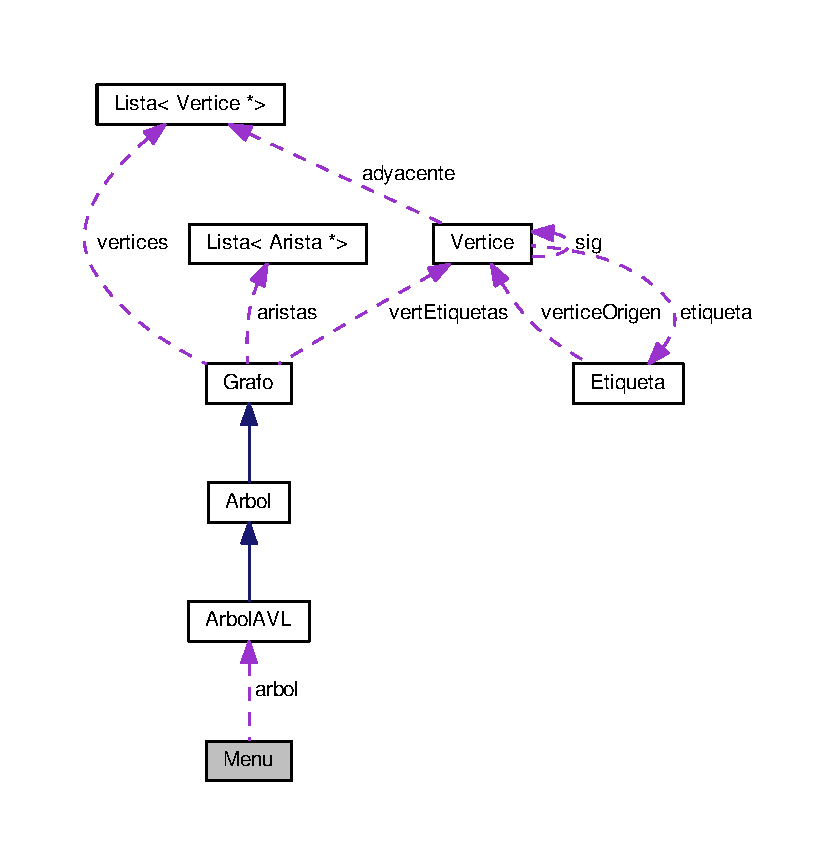
\includegraphics[width=350pt]{classMenu__coll__graph}
\end{center}
\end{figure}
\subsection*{Métodos públicos}
\begin{DoxyCompactItemize}
\item 
\hyperlink{classMenu_a6d615b4b49c03a0cbfc2a01cfae8a64f}{Menu} (\hyperlink{classArbolAVL}{Arbol\+A\+VL} $\ast$a)
\begin{DoxyCompactList}\small\item\em Constructor. \end{DoxyCompactList}\item 
\hyperlink{classMenu_ad673482d111ee4a4d918653df02369e3}{Menu} (\hyperlink{classArbolAVL}{Arbol\+A\+VL} $\ast$a, std\+::string \hyperlink{classMenu_a16f1a749e7d6f35d9c1b4b7ae93b204f}{titulo})
\begin{DoxyCompactList}\small\item\em Constructor. \end{DoxyCompactList}\item 
void \hyperlink{classMenu_a1e1f674058f3fd03a500859abda7dded}{agregar\+\_\+opcion} (std\+::string \hyperlink{classMenu_a16f1a749e7d6f35d9c1b4b7ae93b204f}{titulo}, std\+::function$<$ bool(\hyperlink{classArbolAVL}{Arbol\+A\+VL} $\ast$a)$>$ $\ast$funcion)
\begin{DoxyCompactList}\small\item\em agrega una opcion al menu \end{DoxyCompactList}\item 
void \hyperlink{classMenu_aa964e3e58eb5c6b63ebadd7f2ec6751a}{imprimir\+\_\+opcion} (string texto)
\begin{DoxyCompactList}\small\item\em Imprime una opcion/texto en el menu con formato. \end{DoxyCompactList}\item 
std\+::string \hyperlink{classMenu_a67ebd3e3bcfe45c99a7c0ff13a5c3ebb}{generar\+\_\+n\+\_\+espacios} (int n)
\begin{DoxyCompactList}\small\item\em genera n espacios en blanco \end{DoxyCompactList}\item 
\mbox{\Hypertarget{classMenu_ab0d231cb7a3783451bd690612ff0f77a}\label{classMenu_ab0d231cb7a3783451bd690612ff0f77a}} 
void \hyperlink{classMenu_ab0d231cb7a3783451bd690612ff0f77a}{imprimir\+\_\+opcion} (\hyperlink{classOpcion}{Opcion} $\ast$op, int ind)
\begin{DoxyCompactList}\small\item\em imprime una opcion con indice \end{DoxyCompactList}\item 
int \hyperlink{classMenu_a909877f977f662803994c67e862b4b87}{mostrar} ()
\begin{DoxyCompactList}\small\item\em Muestra el menu de manera elegante. \end{DoxyCompactList}\item 
bool \hyperlink{classMenu_ab5609ebe5415d2e5f06143819b832981}{accion} ()
\begin{DoxyCompactList}\small\item\em Ejecuta la accion actual ingresada por el usuario. \end{DoxyCompactList}\item 
\mbox{\Hypertarget{classMenu_aa6be64bbaaaa59e535507d868cc9740f}\label{classMenu_aa6be64bbaaaa59e535507d868cc9740f}} 
void \hyperlink{classMenu_aa6be64bbaaaa59e535507d868cc9740f}{ejecutar} ()
\begin{DoxyCompactList}\small\item\em Ejecuta el menu mientras el usuario siga realizando operaciones. \end{DoxyCompactList}\end{DoxyCompactItemize}
\subsection*{Atributos públicos}
\begin{DoxyCompactItemize}
\item 
\mbox{\Hypertarget{classMenu_a0b2445d309a32befdc877e64f555a024}\label{classMenu_a0b2445d309a32befdc877e64f555a024}} 
\hyperlink{classArbolAVL}{Arbol\+A\+VL} $\ast$ \hyperlink{classMenu_a0b2445d309a32befdc877e64f555a024}{arbol}
\begin{DoxyCompactList}\small\item\em puntero a arbol sobre el que se va a operar \end{DoxyCompactList}\item 
\mbox{\Hypertarget{classMenu_a16f1a749e7d6f35d9c1b4b7ae93b204f}\label{classMenu_a16f1a749e7d6f35d9c1b4b7ae93b204f}} 
std\+::string \hyperlink{classMenu_a16f1a749e7d6f35d9c1b4b7ae93b204f}{titulo}
\begin{DoxyCompactList}\small\item\em titulo del menu en el programa \end{DoxyCompactList}\end{DoxyCompactItemize}


\subsection{Descripción detallada}
Muestra un menu de opciones automaticamente y ejecuta el codigo que se le indica mediante funciones lambda en cada opcion. 

Definición en la línea 48 del archivo menu.\+hpp.



\subsection{Documentación del constructor y destructor}
\mbox{\Hypertarget{classMenu_a6d615b4b49c03a0cbfc2a01cfae8a64f}\label{classMenu_a6d615b4b49c03a0cbfc2a01cfae8a64f}} 
\index{Menu@{Menu}!Menu@{Menu}}
\index{Menu@{Menu}!Menu@{Menu}}
\subsubsection{\texorpdfstring{Menu()}{Menu()}\hspace{0.1cm}{\footnotesize\ttfamily [1/2]}}
{\footnotesize\ttfamily Menu\+::\+Menu (\begin{DoxyParamCaption}\item[{\hyperlink{classArbolAVL}{Arbol\+A\+VL} $\ast$}]{a }\end{DoxyParamCaption})\hspace{0.3cm}{\ttfamily [inline]}}



Constructor. 


\begin{DoxyParams}{Parámetros}
{\em a} & puntero a \hyperlink{classArbolAVL}{Arbol\+A\+VL} \\
\hline
\end{DoxyParams}


Definición en la línea 62 del archivo menu.\+hpp.

\mbox{\Hypertarget{classMenu_ad673482d111ee4a4d918653df02369e3}\label{classMenu_ad673482d111ee4a4d918653df02369e3}} 
\index{Menu@{Menu}!Menu@{Menu}}
\index{Menu@{Menu}!Menu@{Menu}}
\subsubsection{\texorpdfstring{Menu()}{Menu()}\hspace{0.1cm}{\footnotesize\ttfamily [2/2]}}
{\footnotesize\ttfamily Menu\+::\+Menu (\begin{DoxyParamCaption}\item[{\hyperlink{classArbolAVL}{Arbol\+A\+VL} $\ast$}]{a,  }\item[{std\+::string}]{titulo }\end{DoxyParamCaption})\hspace{0.3cm}{\ttfamily [inline]}}



Constructor. 


\begin{DoxyParams}{Parámetros}
{\em a} & puntero a arbol\+A\+VL \\
\hline
{\em titulo} & titulo del menu en el programa \\
\hline
\end{DoxyParams}


Definición en la línea 69 del archivo menu.\+hpp.



\subsection{Documentación de las funciones miembro}
\mbox{\Hypertarget{classMenu_ab5609ebe5415d2e5f06143819b832981}\label{classMenu_ab5609ebe5415d2e5f06143819b832981}} 
\index{Menu@{Menu}!accion@{accion}}
\index{accion@{accion}!Menu@{Menu}}
\subsubsection{\texorpdfstring{accion()}{accion()}}
{\footnotesize\ttfamily bool Menu\+::accion (\begin{DoxyParamCaption}{ }\end{DoxyParamCaption})\hspace{0.3cm}{\ttfamily [inline]}}



Ejecuta la accion actual ingresada por el usuario. 

\begin{DoxyReturn}{Devuelve}
{\itshape true} si la opcion fue ejecutada {\itshape false} si no se encontro la opcion 
\end{DoxyReturn}


Definición en la línea 155 del archivo menu.\+hpp.

\mbox{\Hypertarget{classMenu_a1e1f674058f3fd03a500859abda7dded}\label{classMenu_a1e1f674058f3fd03a500859abda7dded}} 
\index{Menu@{Menu}!agregar\+\_\+opcion@{agregar\+\_\+opcion}}
\index{agregar\+\_\+opcion@{agregar\+\_\+opcion}!Menu@{Menu}}
\subsubsection{\texorpdfstring{agregar\+\_\+opcion()}{agregar\_opcion()}}
{\footnotesize\ttfamily void Menu\+::agregar\+\_\+opcion (\begin{DoxyParamCaption}\item[{std\+::string}]{titulo,  }\item[{std\+::function$<$ bool(\hyperlink{classArbolAVL}{Arbol\+A\+VL} $\ast$a)$>$ $\ast$}]{funcion }\end{DoxyParamCaption})\hspace{0.3cm}{\ttfamily [inline]}}



agrega una opcion al menu 


\begin{DoxyParams}{Parámetros}
{\em titulo} & titulo de la opcion en el menu \\
\hline
{\em funcion} & funcion que se ejecuta al seleccionar esta opcion \\
\hline
\end{DoxyParams}


Definición en la línea 77 del archivo menu.\+hpp.

\mbox{\Hypertarget{classMenu_a67ebd3e3bcfe45c99a7c0ff13a5c3ebb}\label{classMenu_a67ebd3e3bcfe45c99a7c0ff13a5c3ebb}} 
\index{Menu@{Menu}!generar\+\_\+n\+\_\+espacios@{generar\+\_\+n\+\_\+espacios}}
\index{generar\+\_\+n\+\_\+espacios@{generar\+\_\+n\+\_\+espacios}!Menu@{Menu}}
\subsubsection{\texorpdfstring{generar\+\_\+n\+\_\+espacios()}{generar\_n\_espacios()}}
{\footnotesize\ttfamily std\+::string Menu\+::generar\+\_\+n\+\_\+espacios (\begin{DoxyParamCaption}\item[{int}]{n }\end{DoxyParamCaption})\hspace{0.3cm}{\ttfamily [inline]}}



genera n espacios en blanco 


\begin{DoxyParams}{Parámetros}
{\em n} & numero de espacios \\
\hline
\end{DoxyParams}
\begin{DoxyReturn}{Devuelve}
string con n espacios en blanco 
\end{DoxyReturn}


Definición en la línea 101 del archivo menu.\+hpp.

\mbox{\Hypertarget{classMenu_aa964e3e58eb5c6b63ebadd7f2ec6751a}\label{classMenu_aa964e3e58eb5c6b63ebadd7f2ec6751a}} 
\index{Menu@{Menu}!imprimir\+\_\+opcion@{imprimir\+\_\+opcion}}
\index{imprimir\+\_\+opcion@{imprimir\+\_\+opcion}!Menu@{Menu}}
\subsubsection{\texorpdfstring{imprimir\+\_\+opcion()}{imprimir\_opcion()}}
{\footnotesize\ttfamily void Menu\+::imprimir\+\_\+opcion (\begin{DoxyParamCaption}\item[{string}]{texto }\end{DoxyParamCaption})\hspace{0.3cm}{\ttfamily [inline]}}



Imprime una opcion/texto en el menu con formato. 


\begin{DoxyParams}{Parámetros}
{\em texto} & texto a imprimir \\
\hline
\end{DoxyParams}


Definición en la línea 89 del archivo menu.\+hpp.

\mbox{\Hypertarget{classMenu_a909877f977f662803994c67e862b4b87}\label{classMenu_a909877f977f662803994c67e862b4b87}} 
\index{Menu@{Menu}!mostrar@{mostrar}}
\index{mostrar@{mostrar}!Menu@{Menu}}
\subsubsection{\texorpdfstring{mostrar()}{mostrar()}}
{\footnotesize\ttfamily int Menu\+::mostrar (\begin{DoxyParamCaption}{ }\end{DoxyParamCaption})\hspace{0.3cm}{\ttfamily [inline]}}



Muestra el menu de manera elegante. 

\begin{DoxyReturn}{Devuelve}
opcion elegida por el usuario 
\end{DoxyReturn}


Definición en la línea 127 del archivo menu.\+hpp.



La documentación para esta clase fue generada a partir del siguiente fichero\+:\begin{DoxyCompactItemize}
\item 
\hyperlink{menu_8hpp}{menu.\+hpp}\end{DoxyCompactItemize}

\hypertarget{classLista_1_1Nodo}{}\section{Referencia de la Clase Lista$<$ tipo $>$\+:\+:Nodo}
\label{classLista_1_1Nodo}\index{Lista$<$ tipo $>$\+::\+Nodo@{Lista$<$ tipo $>$\+::\+Nodo}}


Clase que funciona como unidad basica en el T\+DA \hyperlink{classLista}{Lista}.  




{\ttfamily \#include $<$lista.\+hpp$>$}



Diagrama de colaboración para Lista$<$ tipo $>$\+:\+:Nodo\+:\nopagebreak
\begin{figure}[H]
\begin{center}
\leavevmode
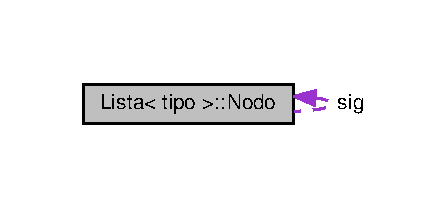
\includegraphics[width=215pt]{classLista_1_1Nodo__coll__graph}
\end{center}
\end{figure}
\subsection*{Métodos públicos}
\begin{DoxyCompactItemize}
\item 
\mbox{\Hypertarget{classLista_1_1Nodo_ada58da3b483872b9b752616a4f736bfe}\label{classLista_1_1Nodo_ada58da3b483872b9b752616a4f736bfe}} 
\hyperlink{classLista_1_1Nodo_ada58da3b483872b9b752616a4f736bfe}{Nodo} ()
\begin{DoxyCompactList}\small\item\em Constructor de la clase \hyperlink{classLista_1_1Nodo}{Nodo}. \end{DoxyCompactList}\item 
\hyperlink{classLista_1_1Nodo_a76d93da356c9904873c409f413737e58}{Nodo} (tipo d)
\begin{DoxyCompactList}\small\item\em Constructor de la clase \hyperlink{classLista_1_1Nodo}{Nodo}. \end{DoxyCompactList}\item 
\hyperlink{classLista_1_1Nodo_a0ab9f1e824afe00a532fabf20ffc2607}{Nodo} (std\+::string \hyperlink{classLista_1_1Nodo_ab6ad6f5015b5e8acd5f82ca3701eb804}{nombre}, tipo d)
\begin{DoxyCompactList}\small\item\em Constructor de la clase \hyperlink{classLista_1_1Nodo}{Nodo}. \end{DoxyCompactList}\end{DoxyCompactItemize}
\subsection*{Atributos públicos}
\begin{DoxyCompactItemize}
\item 
\mbox{\Hypertarget{classLista_1_1Nodo_a8594ea833e1be652cb7a9b8be66bf97d}\label{classLista_1_1Nodo_a8594ea833e1be652cb7a9b8be66bf97d}} 
\hyperlink{classLista_1_1Nodo}{Nodo} $\ast$ \hyperlink{classLista_1_1Nodo_a8594ea833e1be652cb7a9b8be66bf97d}{sig}
\begin{DoxyCompactList}\small\item\em $<$ Capo siguiente de nodo \end{DoxyCompactList}\item 
\mbox{\Hypertarget{classLista_1_1Nodo_ae3e8f0073984b0791ba94590ea9e2c9f}\label{classLista_1_1Nodo_ae3e8f0073984b0791ba94590ea9e2c9f}} 
tipo \hyperlink{classLista_1_1Nodo_ae3e8f0073984b0791ba94590ea9e2c9f}{dato}
\begin{DoxyCompactList}\small\item\em $<$ Dato cualquiera \end{DoxyCompactList}\item 
\mbox{\Hypertarget{classLista_1_1Nodo_ab6ad6f5015b5e8acd5f82ca3701eb804}\label{classLista_1_1Nodo_ab6ad6f5015b5e8acd5f82ca3701eb804}} 
std\+::string \hyperlink{classLista_1_1Nodo_ab6ad6f5015b5e8acd5f82ca3701eb804}{nombre}
\begin{DoxyCompactList}\small\item\em $<$ Nombre del nodo \end{DoxyCompactList}\end{DoxyCompactItemize}


\subsection{Descripción detallada}
\subsubsection*{template$<$typename tipo$>$\newline
class Lista$<$ tipo $>$\+::\+Nodo}

Clase que funciona como unidad basica en el T\+DA \hyperlink{classLista}{Lista}. 

Definición en la línea 150 del archivo lista.\+hpp.



\subsection{Documentación del constructor y destructor}
\mbox{\Hypertarget{classLista_1_1Nodo_a76d93da356c9904873c409f413737e58}\label{classLista_1_1Nodo_a76d93da356c9904873c409f413737e58}} 
\index{Lista\+::\+Nodo@{Lista\+::\+Nodo}!Nodo@{Nodo}}
\index{Nodo@{Nodo}!Lista\+::\+Nodo@{Lista\+::\+Nodo}}
\subsubsection{\texorpdfstring{Nodo()}{Nodo()}\hspace{0.1cm}{\footnotesize\ttfamily [1/2]}}
{\footnotesize\ttfamily template$<$typename tipo$>$ \\
\hyperlink{classLista}{Lista}$<$ tipo $>$\+::Nodo\+::\+Nodo (\begin{DoxyParamCaption}\item[{tipo}]{d }\end{DoxyParamCaption})\hspace{0.3cm}{\ttfamily [inline]}}



Constructor de la clase \hyperlink{classLista_1_1Nodo}{Nodo}. 


\begin{DoxyParams}{Parámetros}
{\em Dato} & \\
\hline
\end{DoxyParams}


Definición en la línea 166 del archivo lista.\+hpp.

\mbox{\Hypertarget{classLista_1_1Nodo_a0ab9f1e824afe00a532fabf20ffc2607}\label{classLista_1_1Nodo_a0ab9f1e824afe00a532fabf20ffc2607}} 
\index{Lista\+::\+Nodo@{Lista\+::\+Nodo}!Nodo@{Nodo}}
\index{Nodo@{Nodo}!Lista\+::\+Nodo@{Lista\+::\+Nodo}}
\subsubsection{\texorpdfstring{Nodo()}{Nodo()}\hspace{0.1cm}{\footnotesize\ttfamily [2/2]}}
{\footnotesize\ttfamily template$<$typename tipo$>$ \\
\hyperlink{classLista}{Lista}$<$ tipo $>$\+::Nodo\+::\+Nodo (\begin{DoxyParamCaption}\item[{std\+::string}]{nombre,  }\item[{tipo}]{d }\end{DoxyParamCaption})\hspace{0.3cm}{\ttfamily [inline]}}



Constructor de la clase \hyperlink{classLista_1_1Nodo}{Nodo}. 


\begin{DoxyParams}{Parámetros}
{\em Nombre} & del nodo \\
\hline
{\em Dato} & \\
\hline
\end{DoxyParams}


Definición en la línea 172 del archivo lista.\+hpp.



La documentación para esta clase fue generada a partir del siguiente fichero\+:\begin{DoxyCompactItemize}
\item 
\hyperlink{lista_8hpp}{lista.\+hpp}\end{DoxyCompactItemize}

\hypertarget{classnodo}{}\section{Referencia de la plantilla de la Clase nodo$<$ T\+I\+PO $>$}
\label{classnodo}\index{nodo$<$ T\+I\+P\+O $>$@{nodo$<$ T\+I\+P\+O $>$}}
\subsection*{Métodos públicos}
\begin{DoxyCompactItemize}
\item 
\mbox{\Hypertarget{classnodo_ad6c42379673cc2de946e77dacace5155}\label{classnodo_ad6c42379673cc2de946e77dacace5155}} 
{\bfseries nodo} (T\+I\+PO v, \hyperlink{classnodo}{nodo}$<$ T\+I\+PO $>$ $\ast$sig=N\+U\+LL)
\end{DoxyCompactItemize}
\subsection*{Amigas}
\begin{DoxyCompactItemize}
\item 
\mbox{\Hypertarget{classnodo_ab6f31a6b425c314a481175b5254170ab}\label{classnodo_ab6f31a6b425c314a481175b5254170ab}} 
class {\bfseries cola$<$ T\+I\+P\+O $>$}
\end{DoxyCompactItemize}


\subsection{Descripción detallada}
\subsubsection*{template$<$class T\+I\+PO$>$\newline
class nodo$<$ T\+I\+P\+O $>$}



Definición en la línea 18 del archivo cola.\+h.



La documentación para esta clase fue generada a partir del siguiente fichero\+:\begin{DoxyCompactItemize}
\item 
cola.\+h\end{DoxyCompactItemize}

\hypertarget{classnodos}{}\section{Referencia de la plantilla de la Clase nodos$<$ T\+I\+PO $>$}
\label{classnodos}\index{nodos$<$ T\+I\+P\+O $>$@{nodos$<$ T\+I\+P\+O $>$}}
\subsection*{Métodos públicos}
\begin{DoxyCompactItemize}
\item 
\mbox{\Hypertarget{classnodos_a4d88f9a2052b194e9ef686407967c254}\label{classnodos_a4d88f9a2052b194e9ef686407967c254}} 
{\bfseries nodos} (T\+I\+PO v, \hyperlink{classnodos}{nodos}$<$ T\+I\+PO $>$ $\ast$sig=N\+U\+LL)
\end{DoxyCompactItemize}
\subsection*{Amigas}
\begin{DoxyCompactItemize}
\item 
\mbox{\Hypertarget{classnodos_ac3309a881bf39610f0c7d0dbb63fbcce}\label{classnodos_ac3309a881bf39610f0c7d0dbb63fbcce}} 
class {\bfseries pila$<$ T\+I\+P\+O $>$}
\end{DoxyCompactItemize}


\subsection{Descripción detallada}
\subsubsection*{template$<$class T\+I\+PO$>$\newline
class nodos$<$ T\+I\+P\+O $>$}



Definición en la línea 20 del archivo pila.\+h.



La documentación para esta clase fue generada a partir del siguiente fichero\+:\begin{DoxyCompactItemize}
\item 
pila.\+h\end{DoxyCompactItemize}

\hypertarget{classOpcion}{}\section{Referencia de la Clase Opcion}
\label{classOpcion}\index{Opcion@{Opcion}}


Representa a una opcion en el menu del programa.  




{\ttfamily \#include $<$menu.\+hpp$>$}

\subsection*{Métodos públicos}
\begin{DoxyCompactItemize}
\item 
\hyperlink{classOpcion_aca1ec1590d4a27e91615ec8af53d2824}{Opcion} (std\+::string \hyperlink{classOpcion_a1d02b7f92549a27f96d434111ede0056}{titulo}, std\+::function$<$ bool(\hyperlink{classArbolAVL}{Arbol\+A\+VL} $\ast$a)$>$ $\ast$\hyperlink{classOpcion_a11149c2d9df3732dfb83727f9df76f05}{funcion})
\begin{DoxyCompactList}\small\item\em Constructor de la clase. \end{DoxyCompactList}\end{DoxyCompactItemize}
\subsection*{Atributos públicos}
\begin{DoxyCompactItemize}
\item 
\mbox{\Hypertarget{classOpcion_a1d02b7f92549a27f96d434111ede0056}\label{classOpcion_a1d02b7f92549a27f96d434111ede0056}} 
std\+::string \hyperlink{classOpcion_a1d02b7f92549a27f96d434111ede0056}{titulo}
\begin{DoxyCompactList}\small\item\em titulo que se muestra en el menu \end{DoxyCompactList}\item 
\mbox{\Hypertarget{classOpcion_a11149c2d9df3732dfb83727f9df76f05}\label{classOpcion_a11149c2d9df3732dfb83727f9df76f05}} 
std\+::function$<$ bool(\hyperlink{classArbolAVL}{Arbol\+A\+VL} $\ast$a)$>$ $\ast$ \hyperlink{classOpcion_a11149c2d9df3732dfb83727f9df76f05}{funcion}
\begin{DoxyCompactList}\small\item\em funcion que ejecuta el codigo de la opcion del menu, cuando se selecciona \end{DoxyCompactList}\end{DoxyCompactItemize}


\subsection{Descripción detallada}
Representa a una opcion en el menu del programa. 

Definición en la línea 21 del archivo menu.\+hpp.



\subsection{Documentación del constructor y destructor}
\mbox{\Hypertarget{classOpcion_aca1ec1590d4a27e91615ec8af53d2824}\label{classOpcion_aca1ec1590d4a27e91615ec8af53d2824}} 
\index{Opcion@{Opcion}!Opcion@{Opcion}}
\index{Opcion@{Opcion}!Opcion@{Opcion}}
\subsubsection{\texorpdfstring{Opcion()}{Opcion()}}
{\footnotesize\ttfamily Opcion\+::\+Opcion (\begin{DoxyParamCaption}\item[{std\+::string}]{titulo,  }\item[{std\+::function$<$ bool(\hyperlink{classArbolAVL}{Arbol\+A\+VL} $\ast$a)$>$ $\ast$}]{funcion }\end{DoxyParamCaption})\hspace{0.3cm}{\ttfamily [inline]}}



Constructor de la clase. 


\begin{DoxyParams}{Parámetros}
{\em titulo} & titulo de la opcion, sin numero ni saltos de linea \\
\hline
{\em funcion} & funcion que se ejecuta al elegir esta opcion en el menu \\
\hline
\end{DoxyParams}


Definición en la línea 38 del archivo menu.\+hpp.



La documentación para esta clase fue generada a partir del siguiente fichero\+:\begin{DoxyCompactItemize}
\item 
\hyperlink{menu_8hpp}{menu.\+hpp}\end{DoxyCompactItemize}

\hypertarget{classpila}{}\section{Referencia de la plantilla de la Clase pila$<$ T\+I\+PO $>$}
\label{classpila}\index{pila$<$ T\+I\+P\+O $>$@{pila$<$ T\+I\+P\+O $>$}}
\subsection*{Métodos públicos}
\begin{DoxyCompactItemize}
\item 
\mbox{\Hypertarget{classpila_a18755d1505a3d0946c1978c571cd456c}\label{classpila_a18755d1505a3d0946c1978c571cd456c}} 
bool {\bfseries vacia} ()
\item 
\mbox{\Hypertarget{classpila_aadc65c1c0f7d355204aa80d0ca10b688}\label{classpila_aadc65c1c0f7d355204aa80d0ca10b688}} 
void {\bfseries apilar} (T\+I\+PO v)
\item 
\mbox{\Hypertarget{classpila_a6024dd235a660c7806e47a36194b97cc}\label{classpila_a6024dd235a660c7806e47a36194b97cc}} 
T\+I\+PO {\bfseries desapilar} ()
\end{DoxyCompactItemize}


\subsection{Descripción detallada}
\subsubsection*{template$<$class T\+I\+PO$>$\newline
class pila$<$ T\+I\+P\+O $>$}



Definición en la línea 16 del archivo pila.\+h.



La documentación para esta clase fue generada a partir del siguiente fichero\+:\begin{DoxyCompactItemize}
\item 
pila.\+h\end{DoxyCompactItemize}

\hypertarget{classVertice}{}\section{Referencia de la Clase Vertice}
\label{classVertice}\index{Vertice@{Vertice}}


Clase encargada de llenar los datos en los Nodos insertados al \hyperlink{classGrafo}{Grafo}.  




{\ttfamily \#include $<$grafo.\+h$>$}



Diagrama de colaboración para Vertice\+:\nopagebreak
\begin{figure}[H]
\begin{center}
\leavevmode
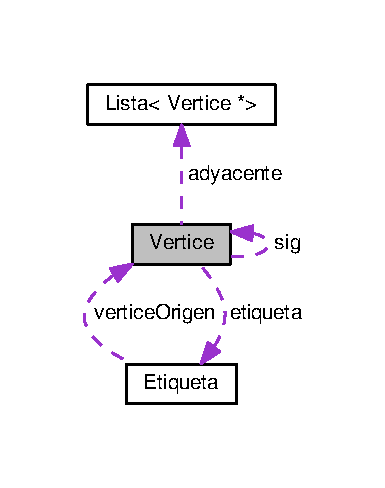
\includegraphics[width=185pt]{classVertice__coll__graph}
\end{center}
\end{figure}
\subsection*{Métodos públicos}
\begin{DoxyCompactItemize}
\item 
\hyperlink{classVertice_a7aff8f5bebd64a371708d72e12edc1dd}{Vertice} (string \hyperlink{classVertice_ab23a005b5c7802792ec2277227ba4d83}{nombre}, int \hyperlink{classVertice_accb96991da9db4ee82280acf2019d1dc}{dato})
\begin{DoxyCompactList}\small\item\em Constructor de \hyperlink{classVertice}{Vertice}. \end{DoxyCompactList}\item 
\mbox{\Hypertarget{classVertice_a9dd7cf987cddf248b9d4e3d31bf8822b}\label{classVertice_a9dd7cf987cddf248b9d4e3d31bf8822b}} 
\hyperlink{classVertice_a9dd7cf987cddf248b9d4e3d31bf8822b}{Vertice} ()
\begin{DoxyCompactList}\small\item\em Atributos de un vértice creado por defecto. \end{DoxyCompactList}\end{DoxyCompactItemize}
\subsection*{Atributos públicos}
\begin{DoxyCompactItemize}
\item 
\mbox{\Hypertarget{classVertice_ad71c11896bd1657ca33117c1c2f08ed3}\label{classVertice_ad71c11896bd1657ca33117c1c2f08ed3}} 
\hyperlink{classVertice}{Vertice} $\ast$ \hyperlink{classVertice_ad71c11896bd1657ca33117c1c2f08ed3}{sig}
\begin{DoxyCompactList}\small\item\em $<$ Se usa para recorrer la lista de vertices \end{DoxyCompactList}\item 
\mbox{\Hypertarget{classVertice_a740d1d3cf0a6fad9b0d49832e8c2cd55}\label{classVertice_a740d1d3cf0a6fad9b0d49832e8c2cd55}} 
\hyperlink{classLista}{Lista}$<$ \hyperlink{classVertice}{Vertice} $\ast$ $>$ $\ast$ \hyperlink{classVertice_a740d1d3cf0a6fad9b0d49832e8c2cd55}{adyacente}
\begin{DoxyCompactList}\small\item\em $<$ \hyperlink{classLista}{Lista} de vértices adyacentes (\hyperlink{classVertice}{Vertice} $\ast$) \end{DoxyCompactList}\item 
\mbox{\Hypertarget{classVertice_ab23a005b5c7802792ec2277227ba4d83}\label{classVertice_ab23a005b5c7802792ec2277227ba4d83}} 
string \hyperlink{classVertice_ab23a005b5c7802792ec2277227ba4d83}{nombre}
\begin{DoxyCompactList}\small\item\em $<$ Nombre que llevará el vértice \end{DoxyCompactList}\item 
\mbox{\Hypertarget{classVertice_accb96991da9db4ee82280acf2019d1dc}\label{classVertice_accb96991da9db4ee82280acf2019d1dc}} 
int \hyperlink{classVertice_accb96991da9db4ee82280acf2019d1dc}{dato}
\begin{DoxyCompactList}\small\item\em $<$ Información que almacena el vértice \end{DoxyCompactList}\item 
\mbox{\Hypertarget{classVertice_af36574fd5dd94e1f7a57ef56e62213e6}\label{classVertice_af36574fd5dd94e1f7a57ef56e62213e6}} 
\hyperlink{classEtiqueta}{Etiqueta} \hyperlink{classVertice_af36574fd5dd94e1f7a57ef56e62213e6}{etiqueta}
\begin{DoxyCompactList}\small\item\em $<$ Creación de un Vértice Origen por defecto \end{DoxyCompactList}\item 
\mbox{\Hypertarget{classVertice_a883addd1f202e3fbae518d32ee933c99}\label{classVertice_a883addd1f202e3fbae518d32ee933c99}} 
bool \hyperlink{classVertice_a883addd1f202e3fbae518d32ee933c99}{visitado}
\begin{DoxyCompactList}\small\item\em $<$ Marca para saber por cuáles vértices ya se ha pasado en los recorridos \end{DoxyCompactList}\end{DoxyCompactItemize}
\subsection*{Amigas}
\begin{DoxyCompactItemize}
\item 
\mbox{\Hypertarget{classVertice_aa89bd7919924d99b99ffa9ab271175a3}\label{classVertice_aa89bd7919924d99b99ffa9ab271175a3}} 
class {\bfseries Grafo}
\item 
ostream \& \hyperlink{classVertice_a3c70523eb9e12f80bb42762ac4708819}{operator$<$$<$} (ostream \&os, const \hyperlink{classVertice}{Vertice} \&v)
\begin{DoxyCompactList}\small\item\em Al momento de llamar a \char`\"{} out $<$$<$ V \char`\"{} donde V es una variable de tipo \hyperlink{classVertice}{Vertice},. \end{DoxyCompactList}\item 
ostream \& \hyperlink{classVertice_a11dd2c98c0d8abf3a52c680bc64ccc87}{operator$<$$<$} (ostream \&os, const \hyperlink{classVertice}{Vertice} $\ast$v)
\begin{DoxyCompactList}\small\item\em Al momento de llamar a \char`\"{} out $<$$<$ V \char`\"{} donde V es una variable de tipo Vertice$\ast$ (apuntador a \hyperlink{classVertice}{Vertice}) (Este es un caso especial para que el grafo muestre los vértices correctamente) \end{DoxyCompactList}\end{DoxyCompactItemize}


\subsection{Descripción detallada}
Clase encargada de llenar los datos en los Nodos insertados al \hyperlink{classGrafo}{Grafo}. 

Definición en la línea 55 del archivo grafo.\+h.



\subsection{Documentación del constructor y destructor}
\mbox{\Hypertarget{classVertice_a7aff8f5bebd64a371708d72e12edc1dd}\label{classVertice_a7aff8f5bebd64a371708d72e12edc1dd}} 
\index{Vertice@{Vertice}!Vertice@{Vertice}}
\index{Vertice@{Vertice}!Vertice@{Vertice}}
\subsubsection{\texorpdfstring{Vertice()}{Vertice()}}
{\footnotesize\ttfamily Vertice\+::\+Vertice (\begin{DoxyParamCaption}\item[{string}]{nombre,  }\item[{int}]{dato }\end{DoxyParamCaption})\hspace{0.3cm}{\ttfamily [inline]}}



Constructor de \hyperlink{classVertice}{Vertice}. 


\begin{DoxyParams}{Parámetros}
{\em nombre} & Forma en la que nos referiremos al vértice \\
\hline
{\em dato} & Información que contendra el vértice \\
\hline
\end{DoxyParams}


Definición en la línea 75 del archivo grafo.\+h.



\subsection{Documentación de las funciones relacionadas y clases amigas}
\mbox{\Hypertarget{classVertice_a3c70523eb9e12f80bb42762ac4708819}\label{classVertice_a3c70523eb9e12f80bb42762ac4708819}} 
\index{Vertice@{Vertice}!operator$<$$<$@{operator$<$$<$}}
\index{operator$<$$<$@{operator$<$$<$}!Vertice@{Vertice}}
\subsubsection{\texorpdfstring{operator$<$$<$}{operator<<}\hspace{0.1cm}{\footnotesize\ttfamily [1/2]}}
{\footnotesize\ttfamily ostream\& operator$<$$<$ (\begin{DoxyParamCaption}\item[{ostream \&}]{os,  }\item[{const \hyperlink{classVertice}{Vertice} \&}]{v }\end{DoxyParamCaption})\hspace{0.3cm}{\ttfamily [friend]}}



Al momento de llamar a \char`\"{} out $<$$<$ V \char`\"{} donde V es una variable de tipo \hyperlink{classVertice}{Vertice},. 

\begin{DoxyReturn}{Devuelve}
Se mostrará en la salida \char`\"{}out\char`\"{} el campo \char`\"{}nombre\char`\"{} de V 
\end{DoxyReturn}


Definición en la línea 88 del archivo grafo.\+h.

\mbox{\Hypertarget{classVertice_a11dd2c98c0d8abf3a52c680bc64ccc87}\label{classVertice_a11dd2c98c0d8abf3a52c680bc64ccc87}} 
\index{Vertice@{Vertice}!operator$<$$<$@{operator$<$$<$}}
\index{operator$<$$<$@{operator$<$$<$}!Vertice@{Vertice}}
\subsubsection{\texorpdfstring{operator$<$$<$}{operator<<}\hspace{0.1cm}{\footnotesize\ttfamily [2/2]}}
{\footnotesize\ttfamily ostream\& operator$<$$<$ (\begin{DoxyParamCaption}\item[{ostream \&}]{os,  }\item[{const \hyperlink{classVertice}{Vertice} $\ast$}]{v }\end{DoxyParamCaption})\hspace{0.3cm}{\ttfamily [friend]}}



Al momento de llamar a \char`\"{} out $<$$<$ V \char`\"{} donde V es una variable de tipo Vertice$\ast$ (apuntador a \hyperlink{classVertice}{Vertice}) (Este es un caso especial para que el grafo muestre los vértices correctamente) 

\begin{DoxyReturn}{Devuelve}
Se mostrará en la salida \char`\"{}out\char`\"{} el campo \char`\"{}nombre\char`\"{} de $\ast$V 
\end{DoxyReturn}


Definición en la línea 97 del archivo grafo.\+h.



La documentación para esta clase fue generada a partir del siguiente fichero\+:\begin{DoxyCompactItemize}
\item 
\hyperlink{grafo_8h}{grafo.\+h}\end{DoxyCompactItemize}

\chapter{Documentación de archivos}
\hypertarget{arbol_8h}{}\section{Referencia del Archivo arbol.\+h}
\label{arbol_8h}\index{arbol.\+h@{arbol.\+h}}


Definción de clase \hyperlink{classArbol}{Arbol} e implementación de sus métodos.  


{\ttfamily \#include $<$iostream$>$}\newline
{\ttfamily \#include $<$cmath$>$}\newline
{\ttfamily \#include $<$string$>$}\newline
{\ttfamily \#include \char`\"{}grafo.\+h\char`\"{}}\newline
{\ttfamily \#include \char`\"{}pila.\+h\char`\"{}}\newline
Dependencia gráfica adjunta para arbol.\+h\+:\nopagebreak
\begin{figure}[H]
\begin{center}
\leavevmode
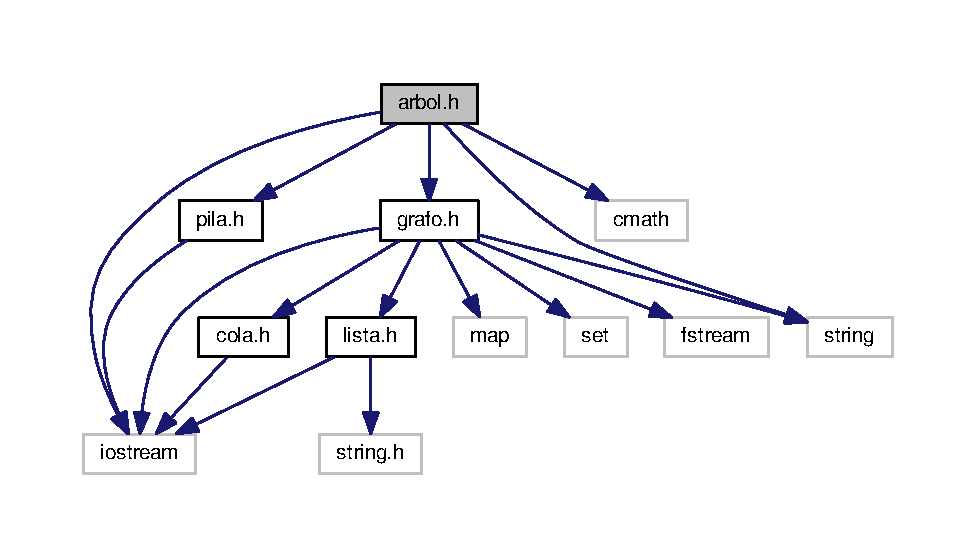
\includegraphics[width=350pt]{arbol_8h__incl}
\end{center}
\end{figure}
Gráfico de los archivos que directa o indirectamente incluyen a este archivo\+:\nopagebreak
\begin{figure}[H]
\begin{center}
\leavevmode
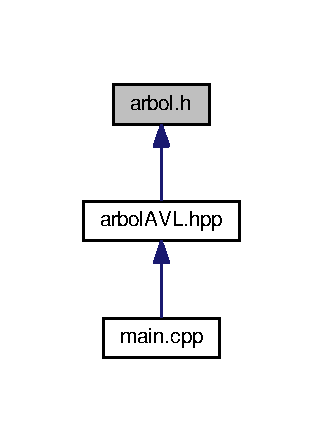
\includegraphics[width=155pt]{arbol_8h__dep__incl}
\end{center}
\end{figure}
\subsection*{Clases}
\begin{DoxyCompactItemize}
\item 
class \hyperlink{classArbol}{Arbol}
\begin{DoxyCompactList}\small\item\em Implementación de un árbol binario con listas de adyacencia. ~\newline
 \end{DoxyCompactList}\end{DoxyCompactItemize}
\subsection*{Funciones}
\begin{DoxyCompactItemize}
\item 
\mbox{\Hypertarget{arbol_8h_a01910d4b2446ba5d0e062ecb24a13b6d}\label{arbol_8h_a01910d4b2446ba5d0e062ecb24a13b6d}} 
bool {\bfseries dos\+\_\+o\+\_\+cero\+\_\+hijos} (\hyperlink{classVertice}{Vertice} $\ast$vert)
\end{DoxyCompactItemize}


\subsection{Descripción detallada}
Definción de clase \hyperlink{classArbol}{Arbol} e implementación de sus métodos. 


\hypertarget{arbolAVL_8hpp}{}\section{Referencia del Archivo arbol\+A\+V\+L.\+hpp}
\label{arbolAVL_8hpp}\index{arbol\+A\+V\+L.\+hpp@{arbol\+A\+V\+L.\+hpp}}


Cabecera de la clase \hyperlink{classArbolAVL}{Arbol\+A\+VL} e implementación de sus métodos.  


{\ttfamily \#include \char`\"{}arbol.\+h\char`\"{}}\newline
{\ttfamily \#include \char`\"{}testing.\+h\char`\"{}}\newline
Dependencia gráfica adjunta para arbol\+A\+V\+L.\+hpp\+:
% FIG 0
Gráfico de los archivos que directa o indirectamente incluyen a este archivo\+:
% FIG 1
\subsection*{Clases}
\begin{DoxyCompactItemize}
\item 
class \hyperlink{classArbolAVL}{Arbol\+A\+VL}
\begin{DoxyCompactList}\small\item\em Implementación de un arbol binario que por cada inserción se corrobore el balance del mismo y se pueda auto-\/balancear. \end{DoxyCompactList}\end{DoxyCompactItemize}


\subsection{Descripción detallada}
Cabecera de la clase \hyperlink{classArbolAVL}{Arbol\+A\+VL} e implementación de sus métodos. 

Archivo de cabecera que contiene la clase \hyperlink{classArbolAVL}{Arbol\+A\+VL}. Esta clase es utilizada para construir árboles binarios {\itshape balanceados} los cuales se dice que están {\itshape balanceados} si su {\bfseries factor de equilibrio} $F_e = \{-1,0,1\}$. ~\newline
 Si el árbol no cuenta con dicho factor de equilibrio, es decir, $F_e = \{ -2,2\}$, se dice que el árbol está {\itshape desbalanceado}. ~\newline
 Cuando el árbol está desbalanceado, según su {\bfseries tipo de desbalance}, se aplica alguna de las cuatro rotaciones que se darán a continuación. Sean $R$ un vértice raíz del subárbol en estudio, $I$ el hijo izquierdo de la raíz y $D$ el hijo derecho de la raíz. Tenemos las siguientes rotaciones según sus factores de equilibrios definidos por $F_e$\+:
\begin{DoxyItemize}
\item Rotación simple izquierda. Esta rotación se aplica cuando $F_e(R) = -2$ y $F_e(I) = -1$
\end{DoxyItemize}




\begin{DoxyItemize}
\item Rotación simple derecha. Esta rotación se aplica cuando $F_e(R) = 2$ y $F_e(D) = 1$
\end{DoxyItemize}




\begin{DoxyItemize}
\item Rotación doble izquierda. Esta rotación se aplica cuando $F_e(R) = 2$ y $F_e(D) = -1$
\end{DoxyItemize}




\begin{DoxyItemize}
\item Rotación doble derecha. Esta rotación se aplica cuando $F_e(R) = -2$ y $F_e(I) = 1$
\end{DoxyItemize}



\begin{DoxySeeAlso}{Ver también}
\hyperlink{classArbolAVL}{Arbol\+A\+VL} 
\end{DoxySeeAlso}

\hypertarget{testing_8h}{}\section{Referencia del Archivo testing.\+h}
\label{testing_8h}\index{testing.\+h@{testing.\+h}}


Cabecera destinada a pruebas de funcionamiento.  


{\ttfamily \#include $<$iostream$>$}\newline
Dependencia gráfica adjunta para testing.\+h\+:\nopagebreak
\begin{figure}[H]
\begin{center}
\leavevmode
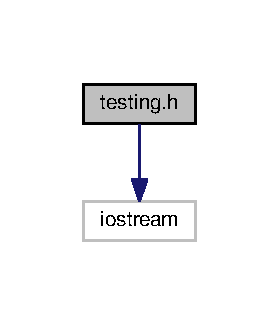
\includegraphics[width=134pt]{testing_8h__incl}
\end{center}
\end{figure}
Gráfico de los archivos que directa o indirectamente incluyen a este archivo\+:\nopagebreak
\begin{figure}[H]
\begin{center}
\leavevmode
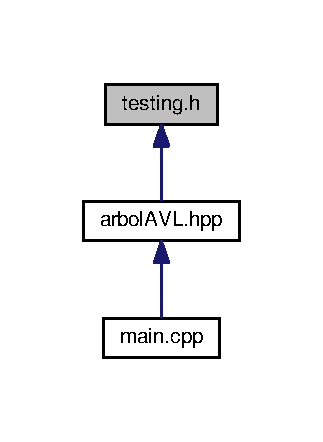
\includegraphics[width=155pt]{testing_8h__dep__incl}
\end{center}
\end{figure}
\subsection*{Namespaces}
\begin{DoxyCompactItemize}
\item 
 \hyperlink{namespacecu}{cu}
\begin{DoxyCompactList}\small\item\em Espacio de nombres destinado a funciones utilizadas en la depuración de las funciones en estudio. \end{DoxyCompactList}\end{DoxyCompactItemize}
\subsection*{defines}
\begin{DoxyCompactItemize}
\item 
\mbox{\Hypertarget{testing_8h_a269aa50758a398403bcc8000fea66075}\label{testing_8h_a269aa50758a398403bcc8000fea66075}} 
\#define {\bfseries T\+E\+S\+T\+\_\+\+N\+U\+LL}~\char`\"{}T\+E\+ST IS N\+U\+LL\char`\"{}
\end{DoxyCompactItemize}
\subsection*{Funciones}
\begin{DoxyCompactItemize}
\item 
void \hyperlink{namespacecu_a2032e7d323896144cae02cca83ea7776}{cu\+::test} (std\+::string str)
\begin{DoxyCompactList}\small\item\em Muestra en consola el texto pasado como parámetro. \end{DoxyCompactList}\item 
void \hyperlink{namespacecu_a29c88a60e2e11b522402097bac91dd53}{cu\+::test} (std\+::string str, std\+::string str2)
\begin{DoxyCompactList}\small\item\em Muestra en consola los textos pasados como parámetro. \end{DoxyCompactList}\item 
void \hyperlink{namespacecu_a204c06884ca90cec812a74a79978ad1b}{cu\+::test} (std\+::string str, int dato)
\begin{DoxyCompactList}\small\item\em Muestra en consola una descripción y un valor dados. \end{DoxyCompactList}\item 
void \hyperlink{namespacecu_ac74aabcdeff59ad38de0aa36237f8a9b}{cu\+::test} (std\+::string str, int dato, int res)
\begin{DoxyCompactList}\small\item\em Muestra en consola una descripción junto con un valor inicial y un valor como resultado. \end{DoxyCompactList}\item 
void \hyperlink{namespacecu_a4f3e4a3066ea798b15af01022a14ecf9}{cu\+::test} (std\+::string str, bool cond, std\+::string msg1, std\+::string msg2)
\begin{DoxyCompactList}\small\item\em Muestra en consola una descripción y, según un valor booleano, decide qué texto mostrar después. \end{DoxyCompactList}\item 
void \hyperlink{namespacecu_af2ea0a4da4f2192d226ca8c3bddbd821}{cu\+::test} (std\+::string str, bool cond)
\begin{DoxyCompactList}\small\item\em Muestra en consola una descripción y, dependiendo del valor booleano dado, mostrará un mensaje \char`\"{}\+Y\+E\+S\char`\"{} o un mensaje \char`\"{}\+N\+O\char`\"{}. \end{DoxyCompactList}\end{DoxyCompactItemize}
\subsection*{Variables}
\begin{DoxyCompactItemize}
\item 
\mbox{\Hypertarget{namespacecu_a67ef22d5c0f232da615812d7c61846a2}\label{namespacecu_a67ef22d5c0f232da615812d7c61846a2}} 
std\+::string \hyperlink{namespacecu_a67ef22d5c0f232da615812d7c61846a2}{cu\+::promt} = \char`\"{}\mbox{[}D\+E\+B\+UG\mbox{]}\char`\"{}
\begin{DoxyCompactList}\small\item\em Texto que indica que se hace referencia a un texto del depurador. \end{DoxyCompactList}\item 
\mbox{\Hypertarget{namespacecu_ae84c5e905dd7b8c2b1b1194553f9c9a9}\label{namespacecu_ae84c5e905dd7b8c2b1b1194553f9c9a9}} 
bool \hyperlink{namespacecu_ae84c5e905dd7b8c2b1b1194553f9c9a9}{cu\+::debug\+\_\+mode} = true
\begin{DoxyCompactList}\small\item\em Booleano que indica si el modo depurador está activado o no, es decir, si está en {\itshape true} o {\itshape false} respectivamente. \end{DoxyCompactList}\end{DoxyCompactItemize}


\subsection{Descripción detallada}
Cabecera destinada a pruebas de funcionamiento. 

Archivo de cabecera que contiene un {\itshape namespace} con métodos utilizados para probar y monitorear el funcionamiento de las funciones en estudio. ~\newline
 Todos los métodos contenidos en él archivo tienen la función de imprimir de manera más práctica en consola mensajes \mbox{[}D\+E\+B\+UG\mbox{]} personalizados por el desarrollador 
%--- End generated contents ---

% Index
\backmatter
\newpage
\phantomsection
\clearemptydoublepage
\addcontentsline{toc}{chapter}{Índice}
\printindex

\end{document}
